%%%%%%%%%%%%%%%%%%%%%%%%%%%%%%%%%%%%%%%%%%%%%%%%%%%%%%%%%%%
\documentclass[xcolor=x11names,compress]{beamer}
%\documentclass[xcolor=x11names,compress, handhouts, aspectratio=169]{beamer}
%% General document
\usepackage{graphicx, subfig}
%% Beamer Layout
\useoutertheme[subsection=false,shadow]{miniframes}
\useinnertheme{default}
\usefonttheme{serif}
\usepackage{palatino}

%%%%%%% Mes Packages %%%%%%%%%%%%%%%%
%\usepackage[french]{babel}
\usepackage[T1]{fontenc}
\usepackage{color}
\usepackage{xcolor}
\usepackage{dsfont} % Pour indicatrice
\usepackage{url}
\usepackage{multirow}
\usepackage[normalem]{ulem}   % For strike out text

% Natbib for clean bibliography
\usepackage[comma,authoryear]{natbib}

%remove the icon
\setbeamertemplate{bibliography item}{}

%remove line breaks
\setbeamertemplate{bibliography entry title}{}
\setbeamertemplate{bibliography entry location}{}
\setbeamertemplate{bibliography entry note}{}

%% ------ MEs couleurs --------
\definecolor{vert}{rgb}{0.1,0.7,0.2}
\definecolor{brique}{rgb}{0.7,0.16,0.16}
\definecolor{gris}{rgb}{0.7, 0.75, 0.71}
\definecolor{twitterblue}{rgb}{0, 0.42, 0.58}
\definecolor{airforceblue}{rgb}{0.36, 0.54, 0.66}
\definecolor{siap}{RGB}{3,133, 200}


%%%%%%%%%%%%%%%%% BEAMER PACKAGE %%%%%%%

\setbeamercolor{itemize item}{fg=siap}
%\setbeamercolor{itemize subitem}{fg=blue}
%\setbeamercolor{itemize subsubitem}{fg=cyan}

\setbeamerfont{title like}{shape=\scshape}
\setbeamerfont{frametitle}{shape=\scshape}

\setbeamercolor*{lower separation line head}{bg=DeepSkyBlue4}
\setbeamercolor*{normal text}{fg=black,bg=white}
\setbeamercolor*{alerted text}{fg=siap}
\setbeamercolor*{example text}{fg=black}
\setbeamercolor*{structure}{fg=black}
\setbeamercolor*{palette tertiary}{fg=black,bg=black!10}
\setbeamercolor*{palette quaternary}{fg=black,bg=black!10}

% Set the header color to SIAP's color
\setbeamercolor*{frametitle}{fg=siap}

%remove navigation symbols
\setbeamertemplate{navigation symbols}{}

\renewcommand{\(}{\begin{columns}}
\renewcommand{\)}{\end{columns}}
\newcommand{\<}[1]{\begin{column}{#1}}
\renewcommand{\>}{\end{column}}

%% Add footer with logo
\setbeamertemplate{footline}{%
  \begin{beamercolorbox}[wd=\paperwidth,ht=2.5ex,dp=1.125ex,%
    leftskip=.3cm,rightskip=.3cm plus1fil]{author in head/foot}
    
\includegraphics[height=5ex]{SIAP-ESCAP-Logo.png}\hfill
    \insertshortauthor\hfill\insertshorttitle\hfill  \textcolor{siap}{\textit{\insertframenumber}}
  \end{beamercolorbox}%
}

% Path for the graphs
\graphicspath{
{Graphics/}
{../Graphics/}
}


\title{\textcolor{siap}{Training on Web Scraping Prices for CPI \\ \vspace{0.5cm} }}

\subtitle{\textcolor{brique}{\Large{ Reproducible Analytical Pipelines}}}
\author{Christophe Bontemps \& Serge Goussev }
\institute{ 
\includegraphics[height=9ex]{SIAP-ESCAP-Logo.png} \hspace{1cm} 
\includegraphics[height=10ex]{StatCanada-Logo.jpg}}
\date{}

\begin{document}

\section{Motivation}

\begin{frame}
  \titlepage
\end{frame}

\begin{frame}{Fundamental Principles of Official Statistics}
  \begin{columns}[T]
    \begin{column}{0.6\textwidth}
      \begin{itemize}[<+->]
        \item Clear mention of the \textbf{processes} used to produce statistics
        \item \emph{To retain trust in official statistics, the \textbf{statistical agencies need to decide} according to strictly professional considerations, including scientific principles and professional ethics, \textbf{on the methods and procedures} for the collection, processing, storage and presentation of statistical data.}
      \item In short, \textbf{processes} are important!
      \end{itemize}
    \end{column}
    \begin{column}{0.4\textwidth}
      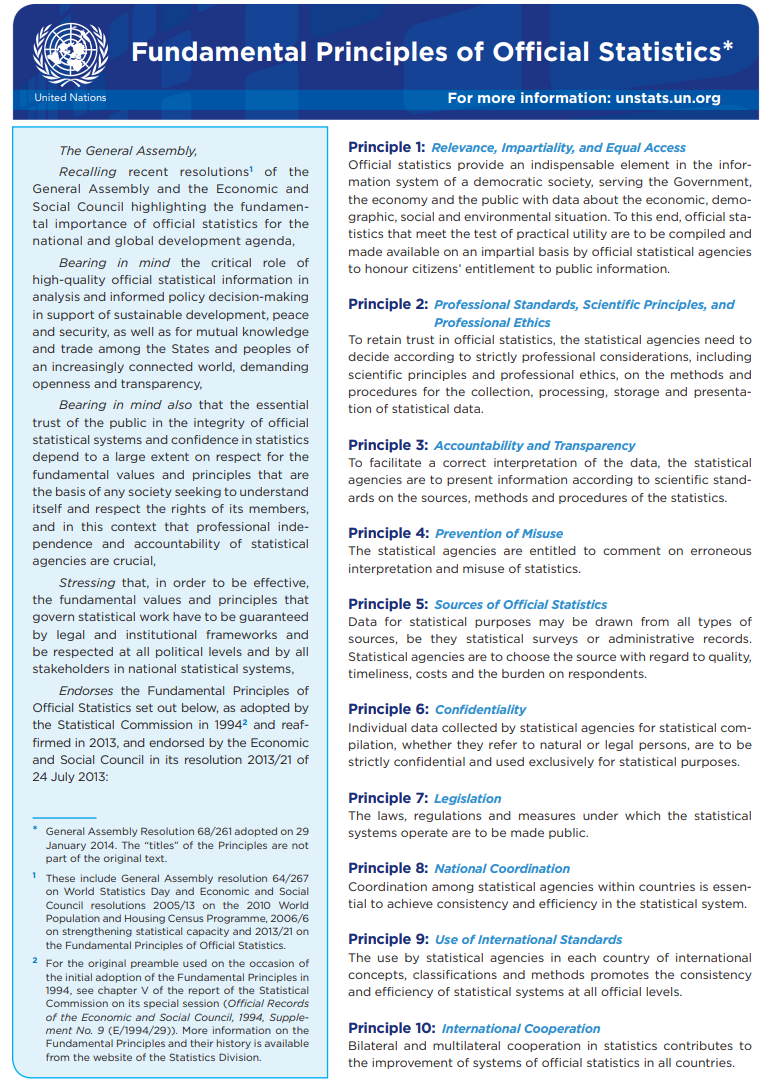
\includegraphics[width=\textwidth]{FundamentalPrinciplesOS.PNG}
    \end{column}
  \end{columns}
\end{frame}

\begin{frame}{Usual practice: Theory vs reality}
\begin{center}
  \begin{itemize}
        \only<1>{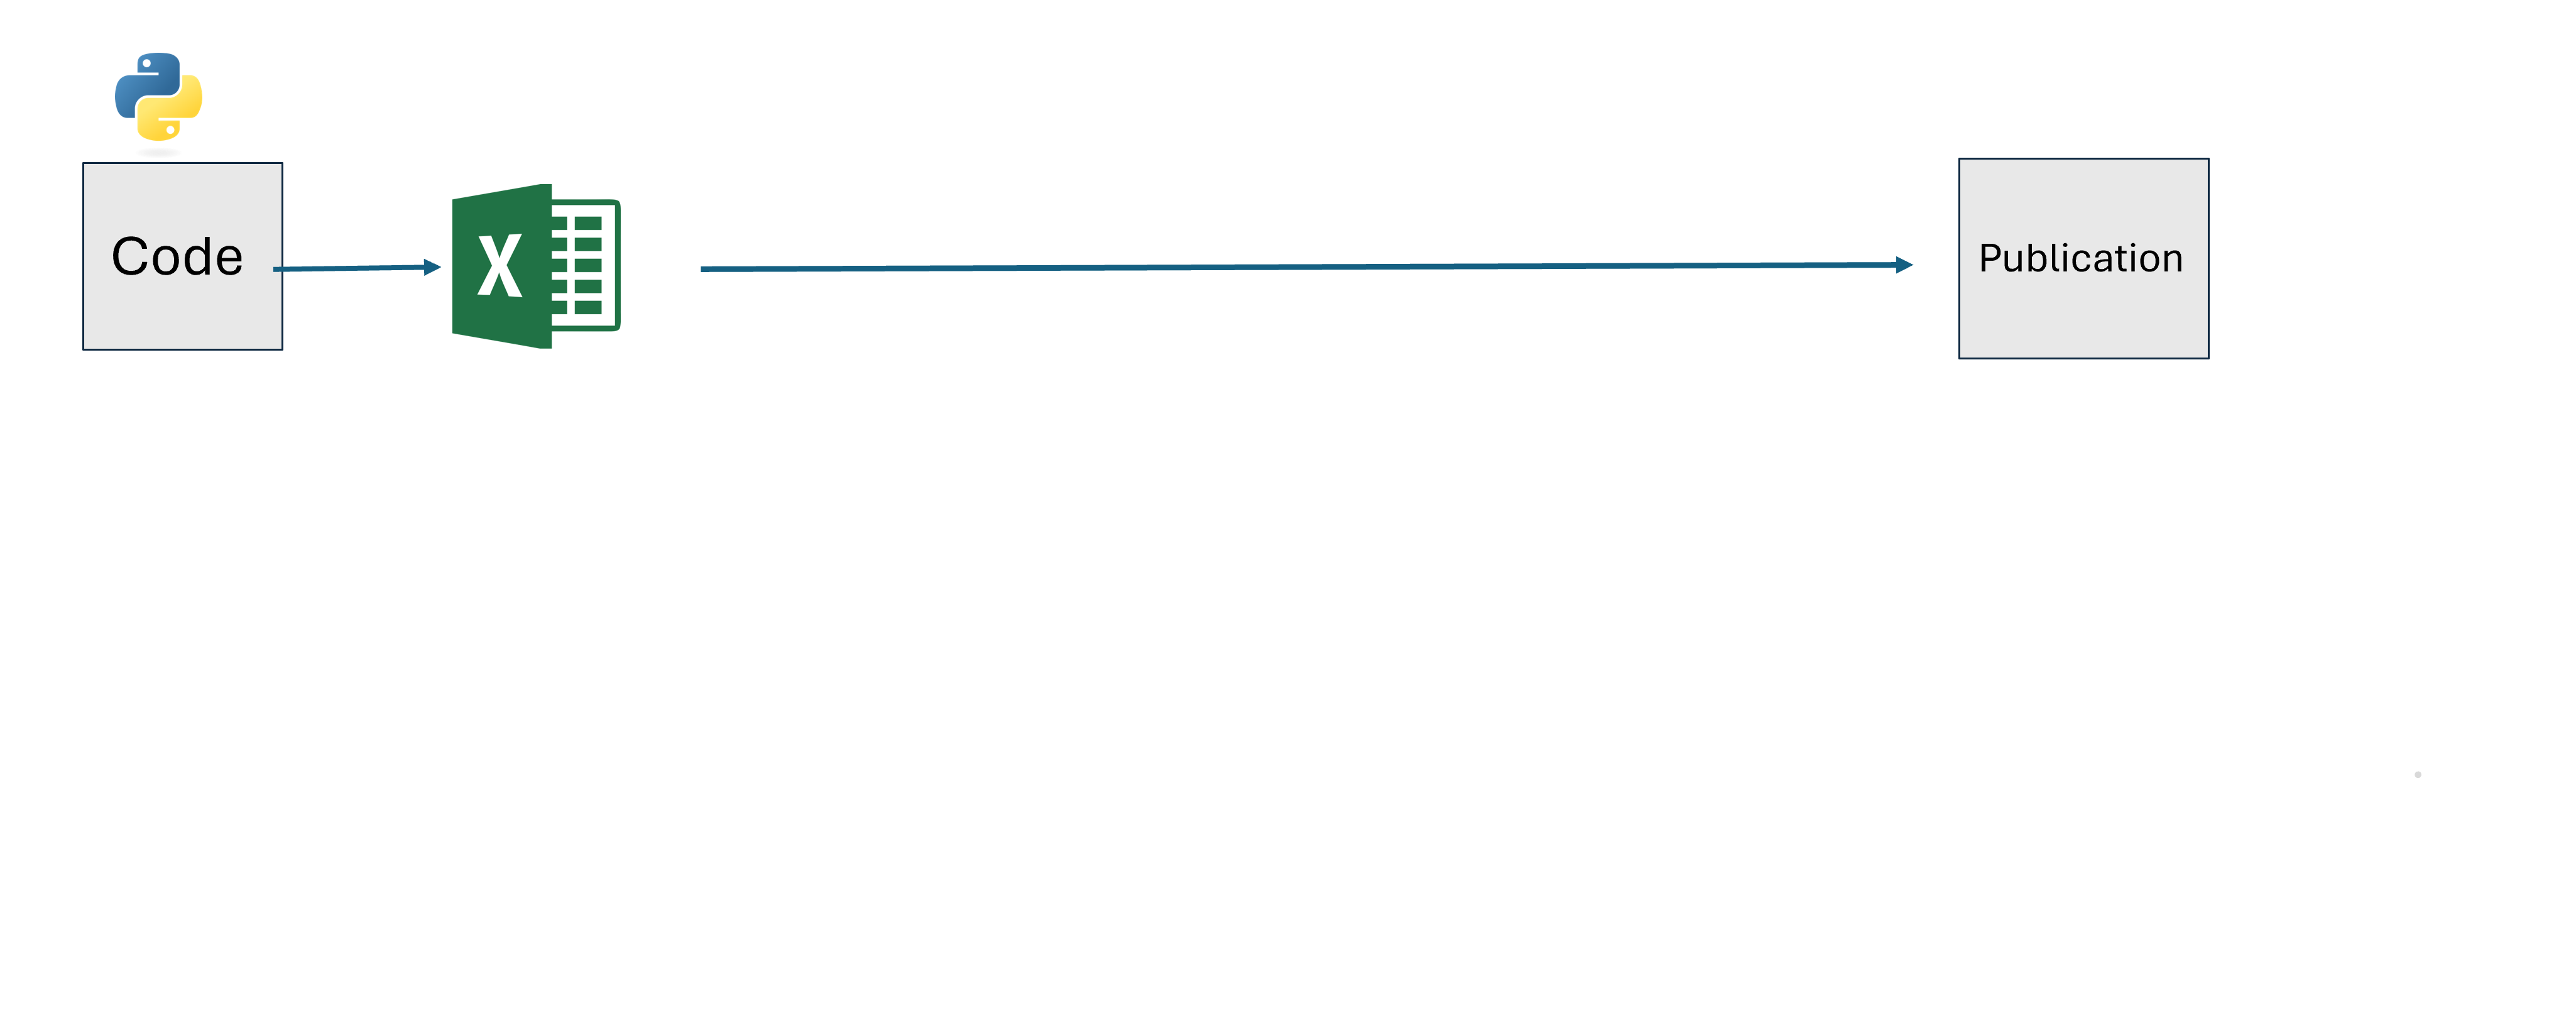
\includegraphics[width=0.8\textwidth]{Process1.png} \\ Comment 1}
        \only<2>{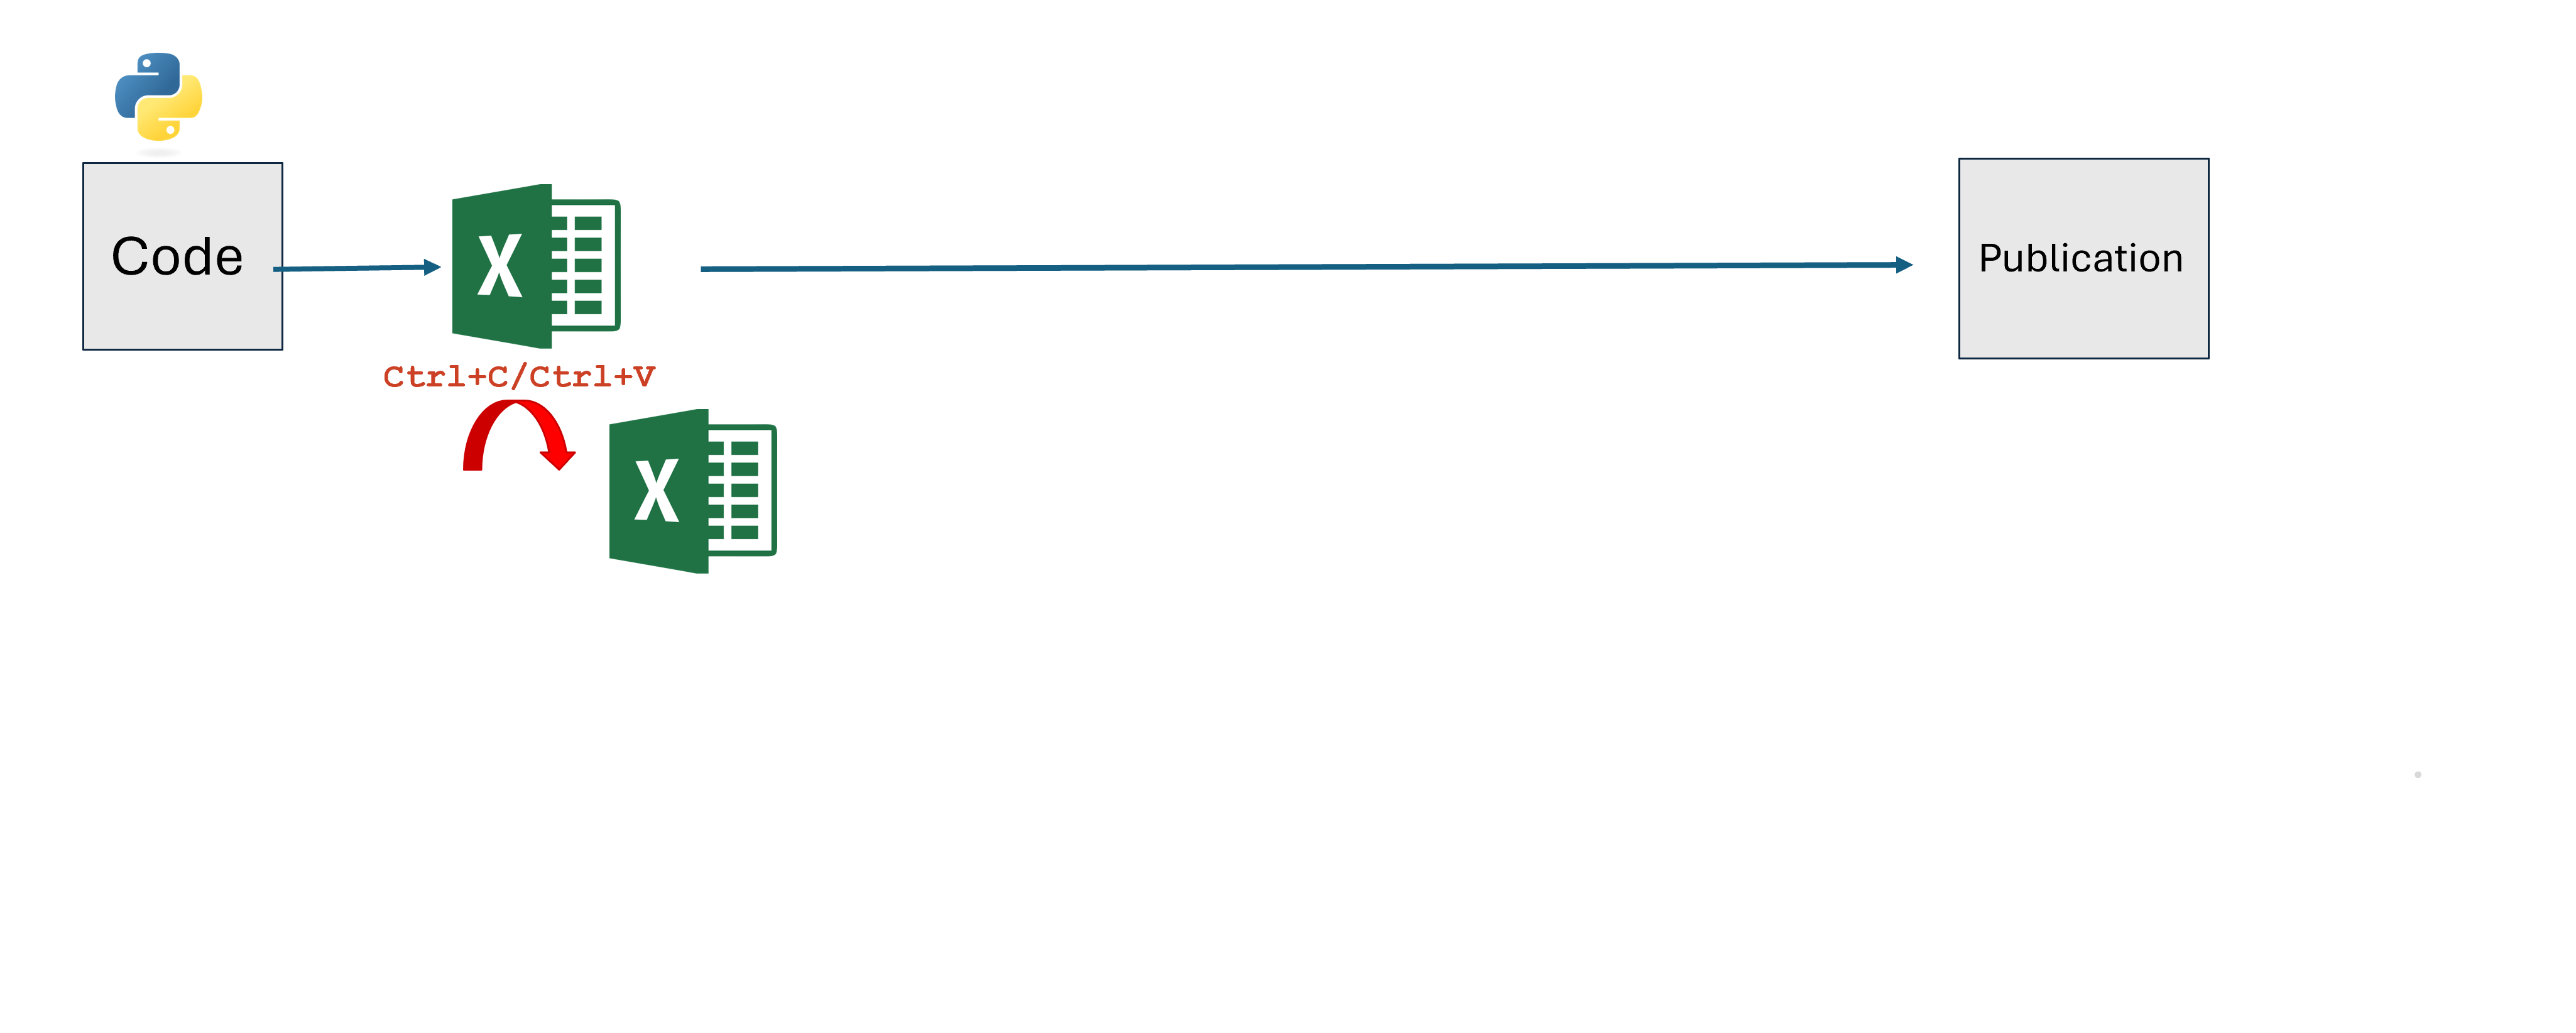
\includegraphics[width=0.8\textwidth]{Process2.png} \\ Comment 2}
        \only<3>{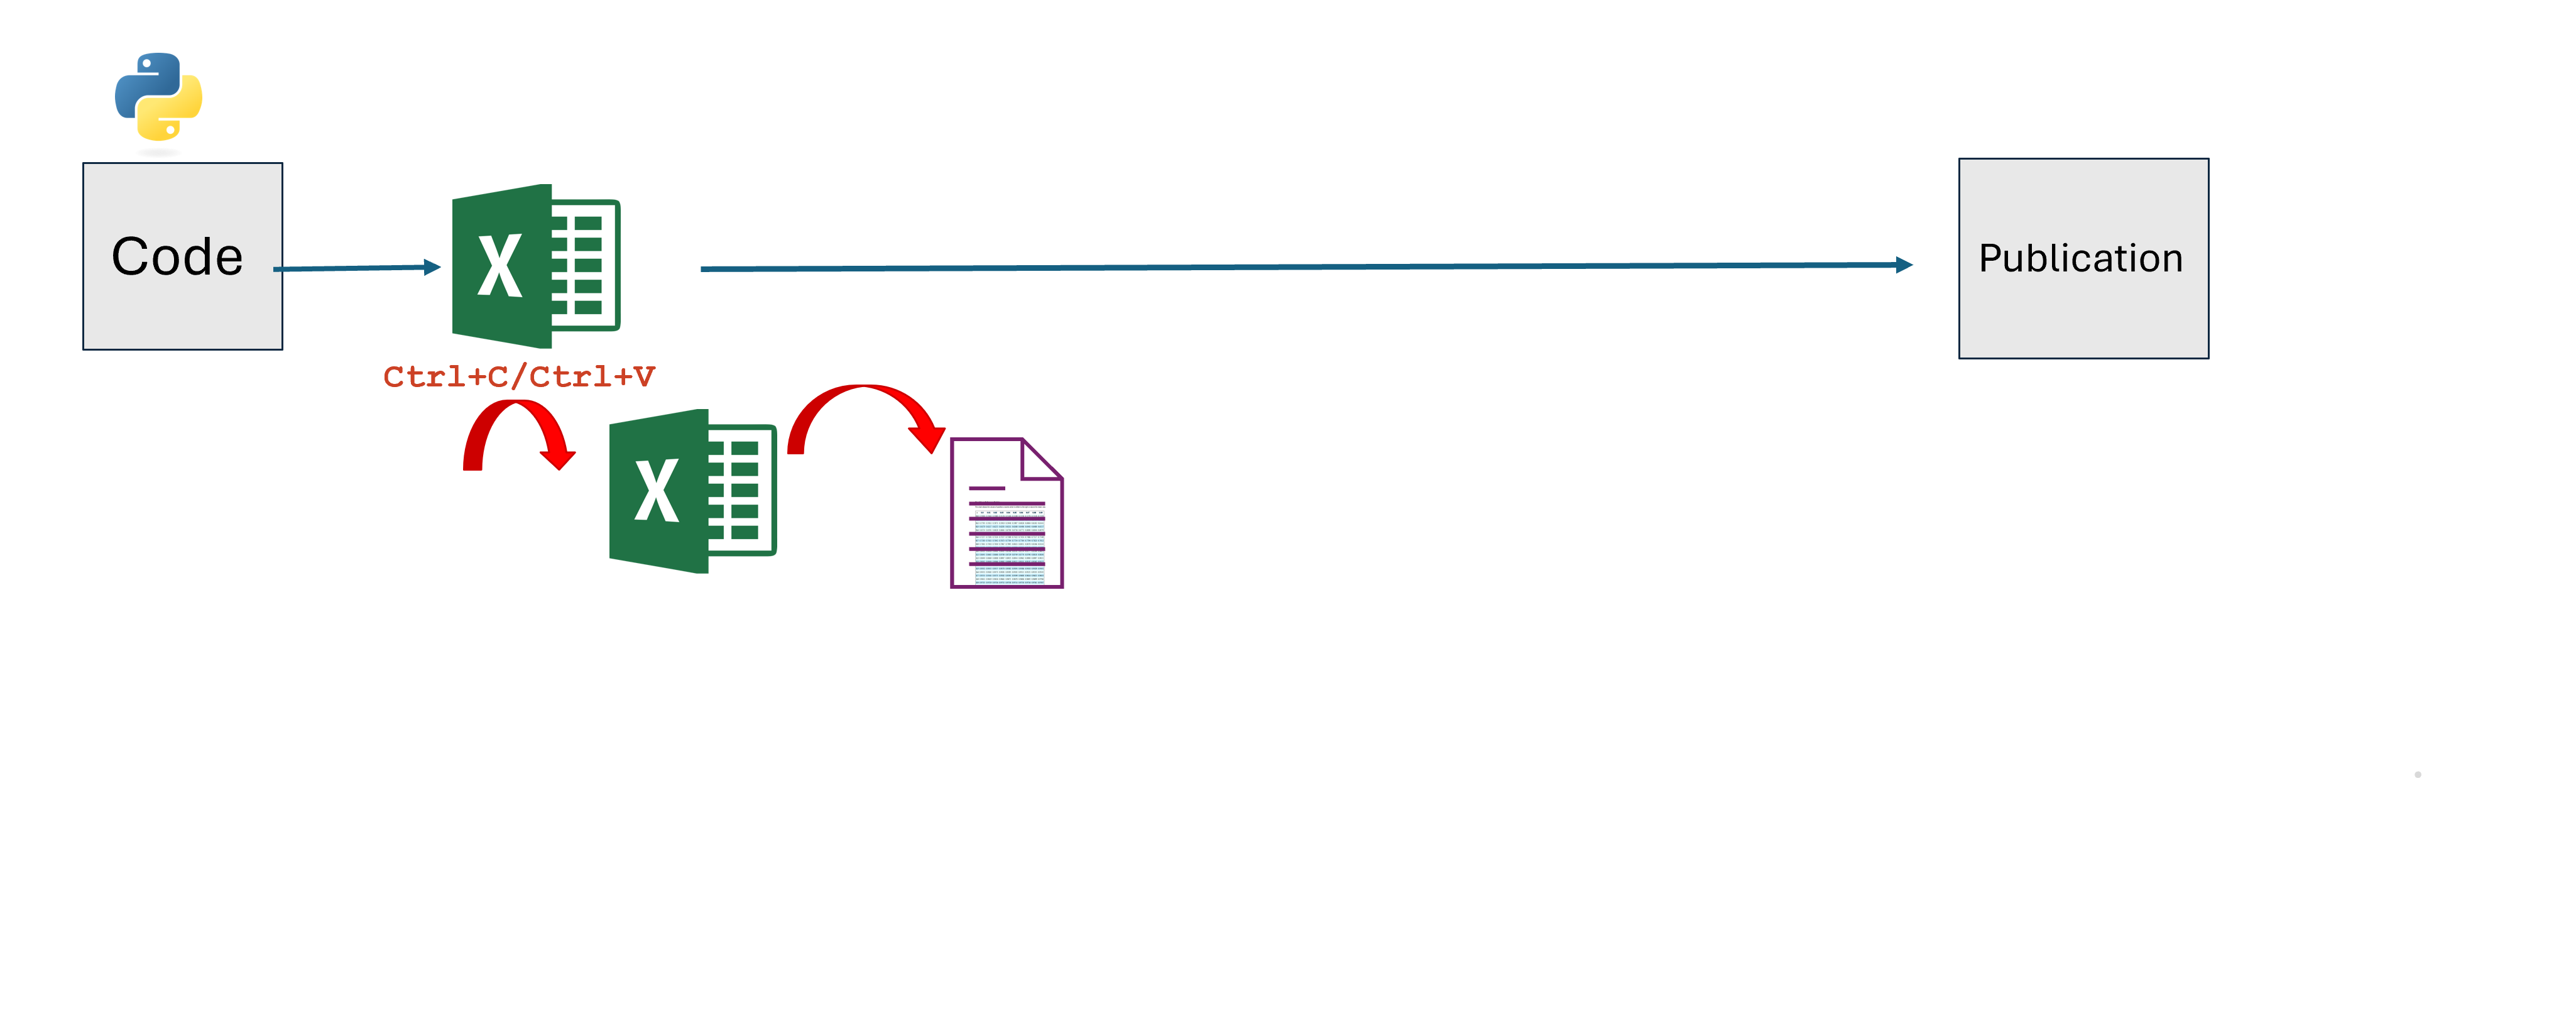
\includegraphics[width=0.8\textwidth]{Process3.png} \\ Comment 3}
        \only<4>{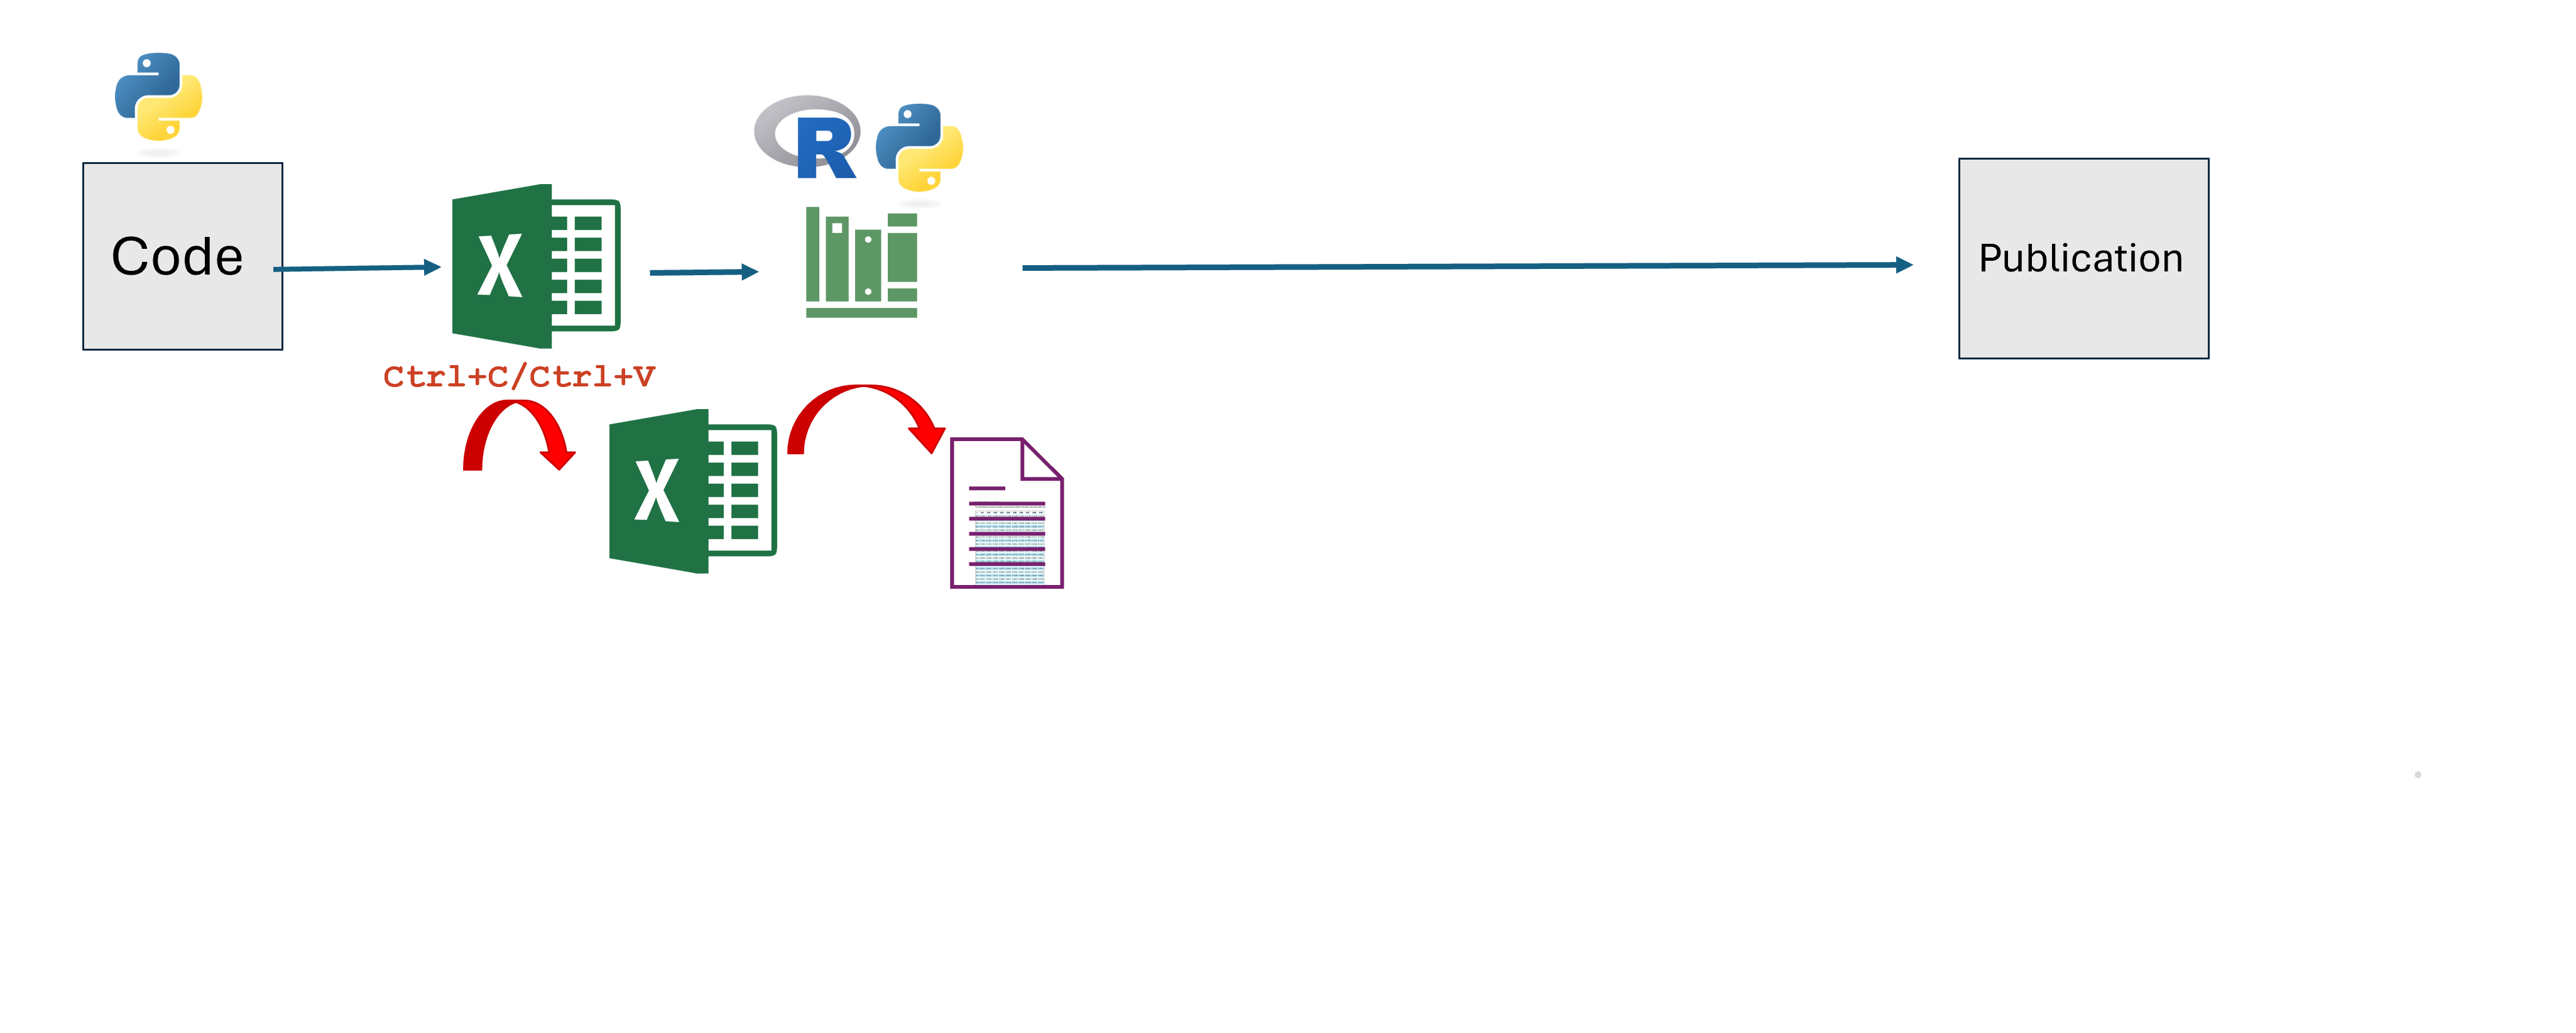
\includegraphics[width=0.8\textwidth]{Process4.png} \\ Comment 4}
        \only<5>{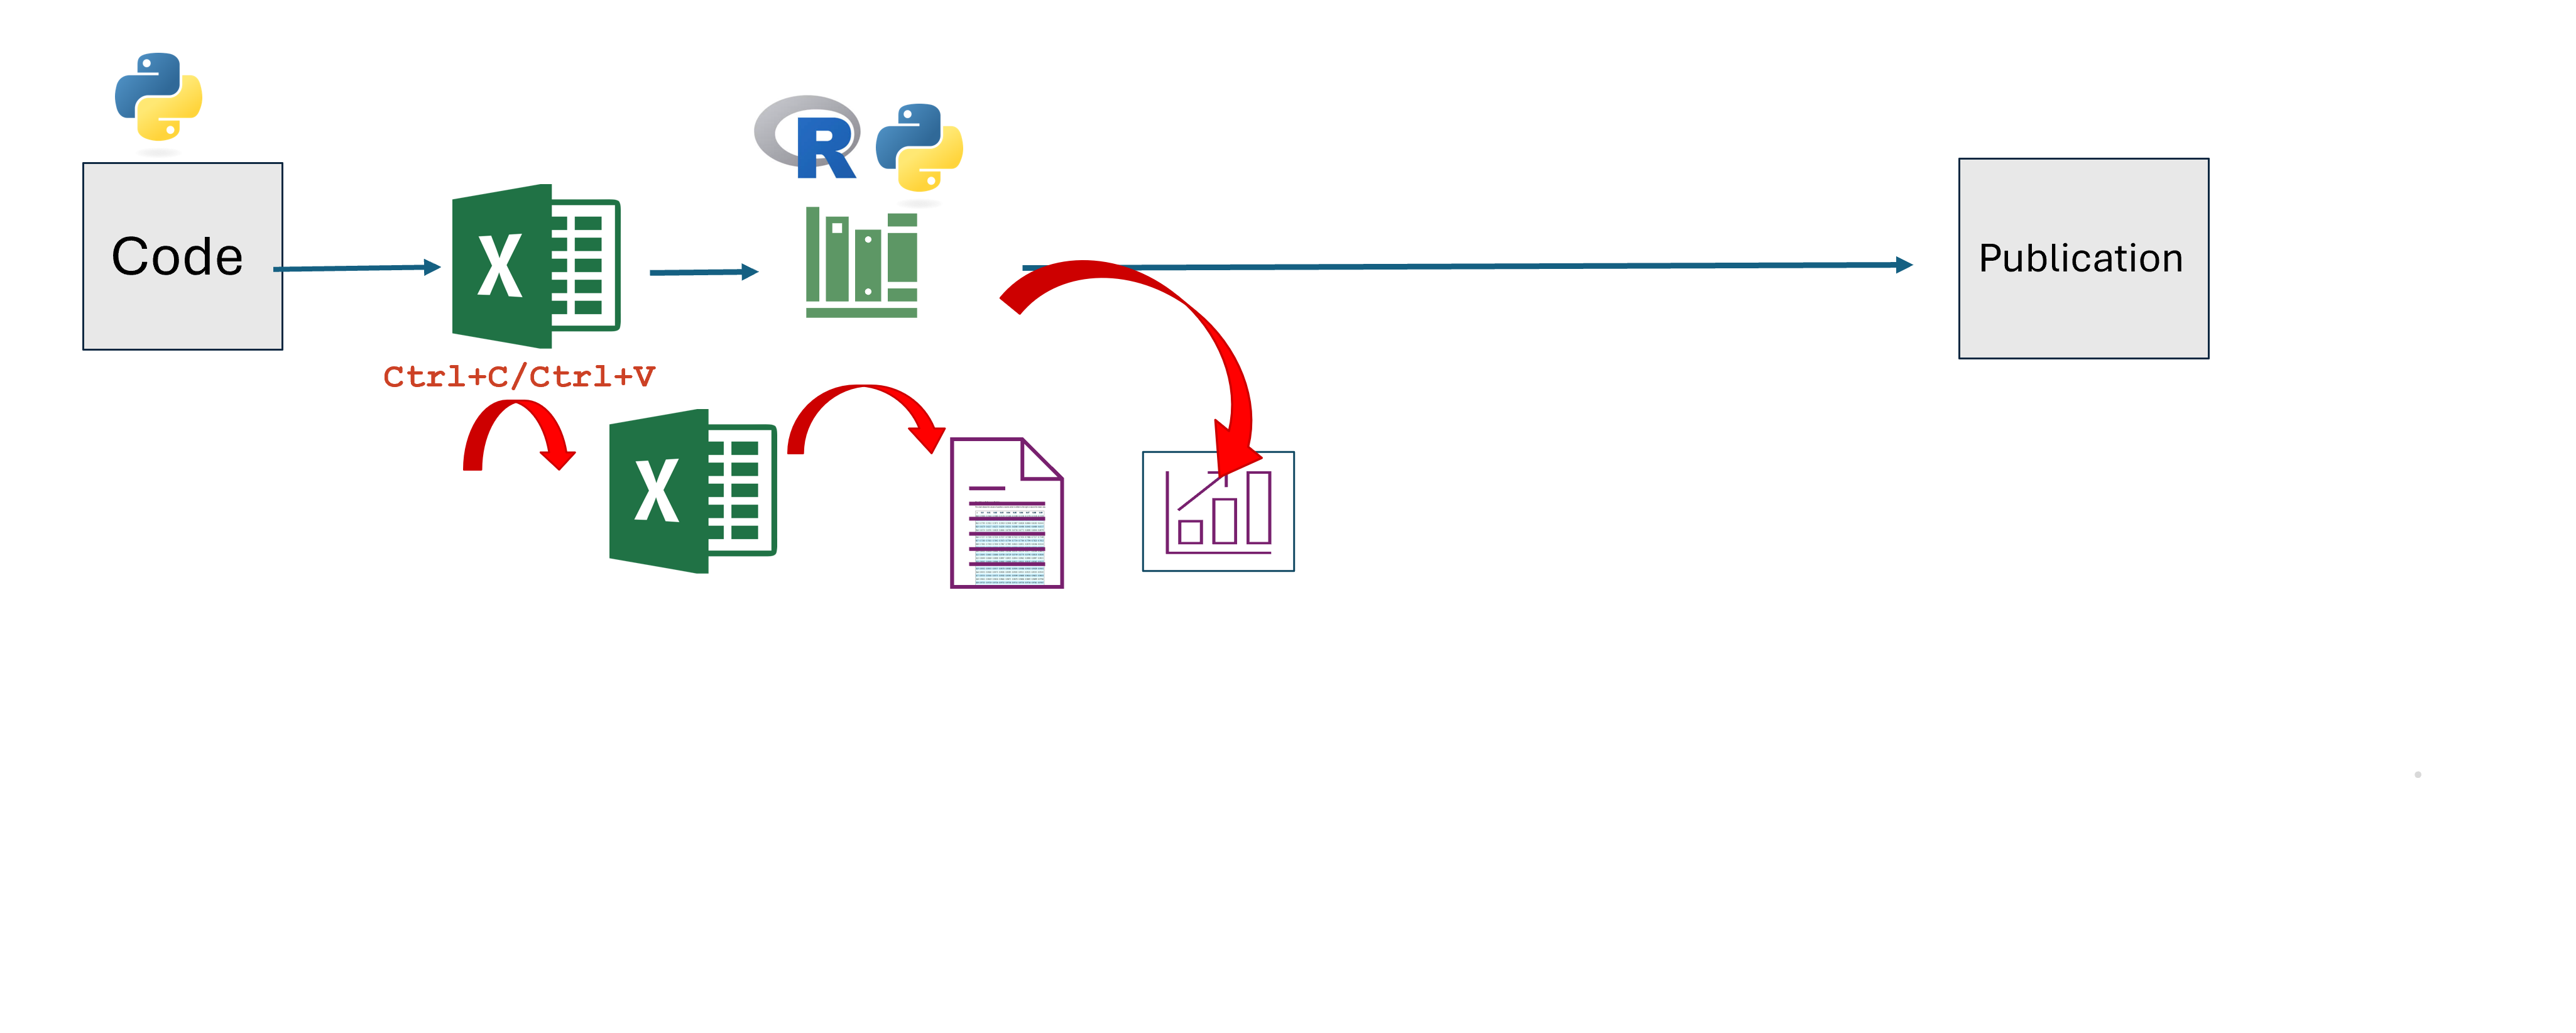
\includegraphics[width=0.8\textwidth]{Process5.png} \\ Comment 5}
        \only<6>{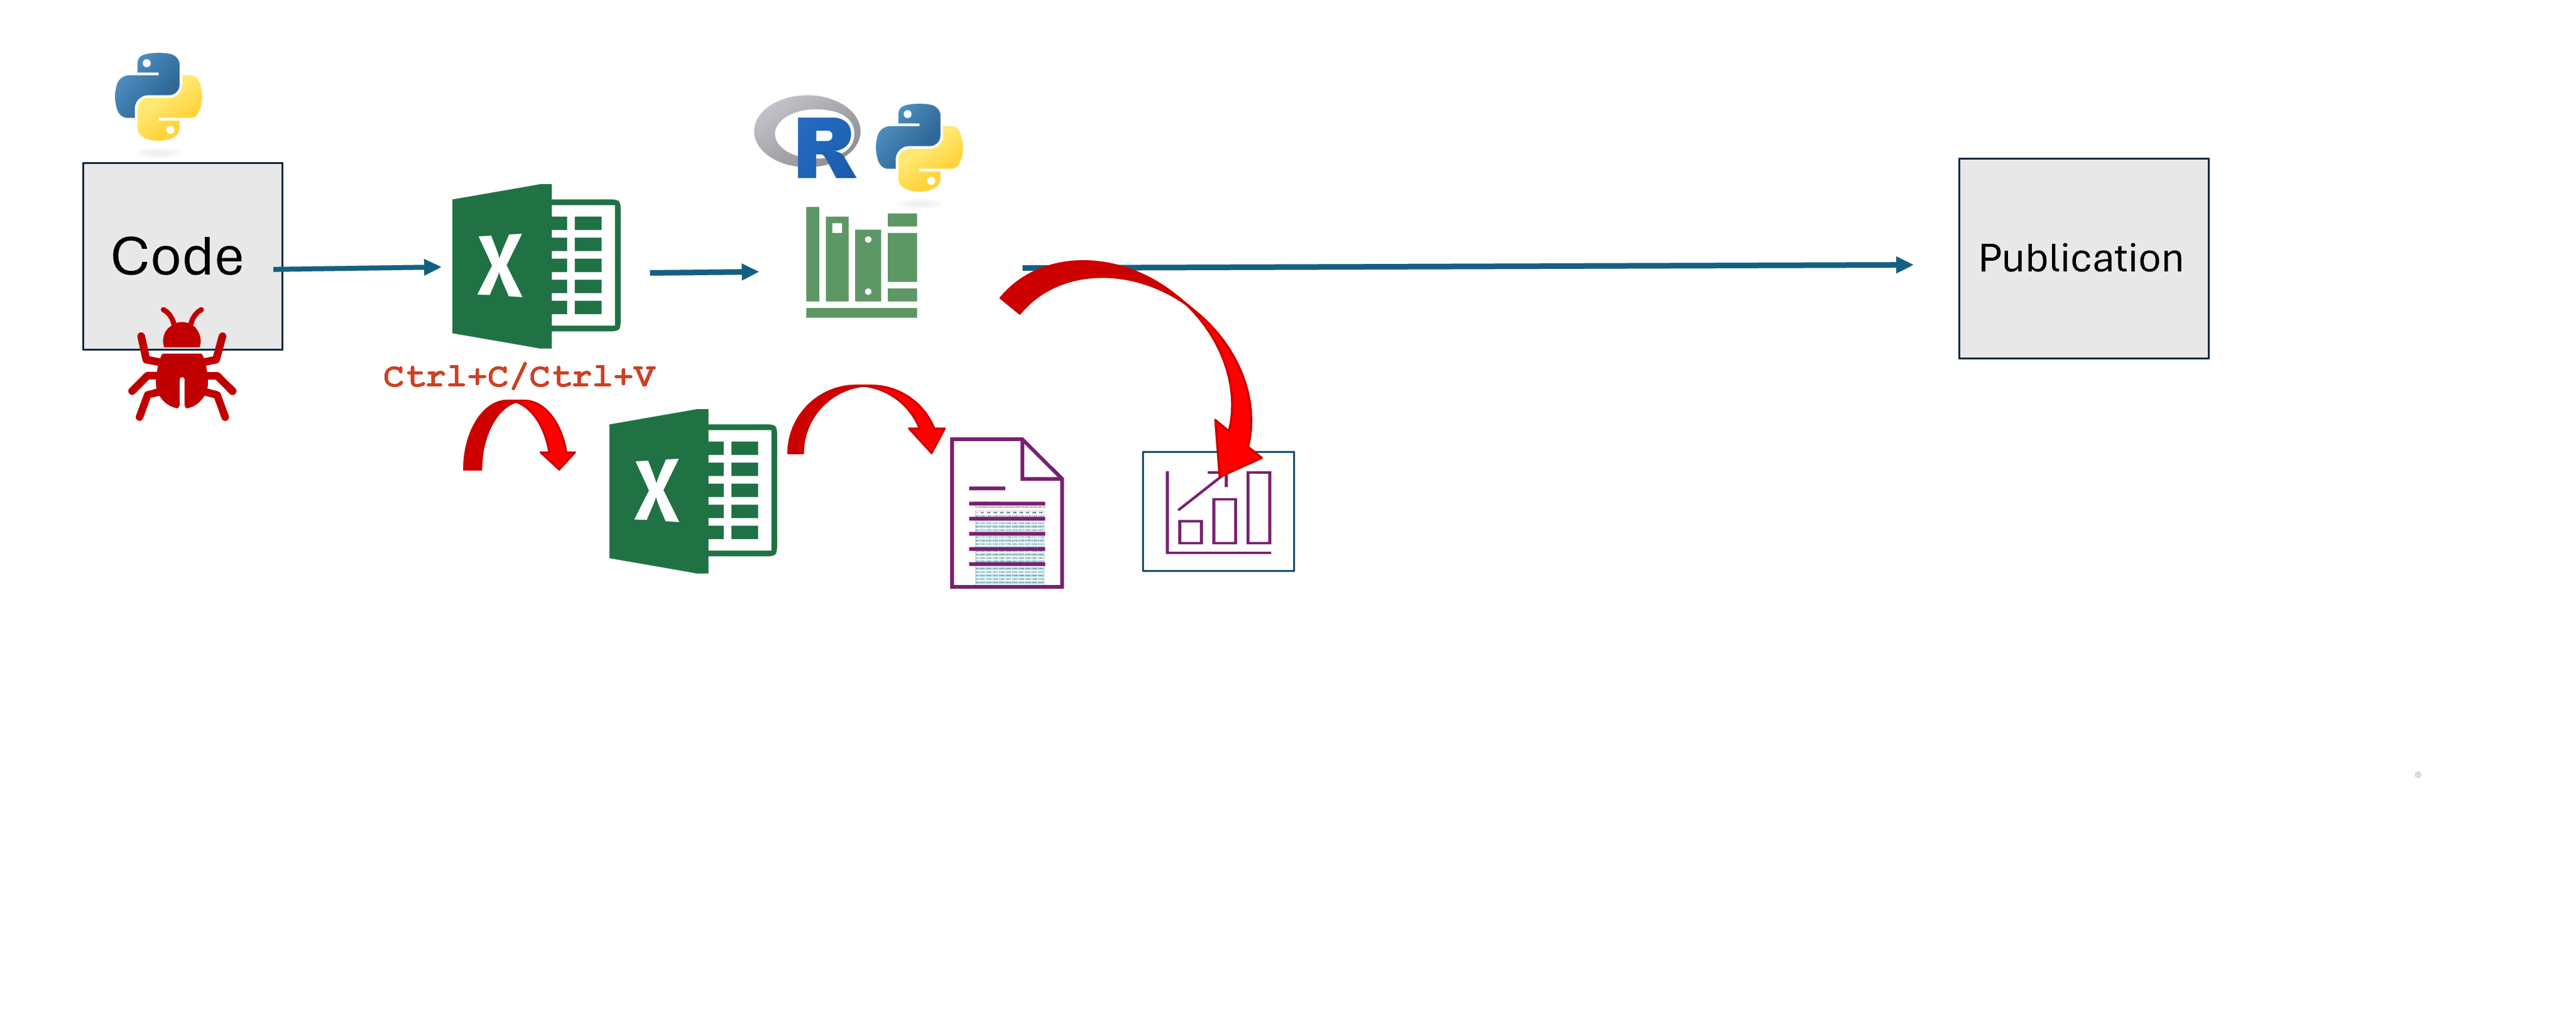
\includegraphics[width=0.8\textwidth]{Process6.png} \\ Comment 6}
        \only<7>{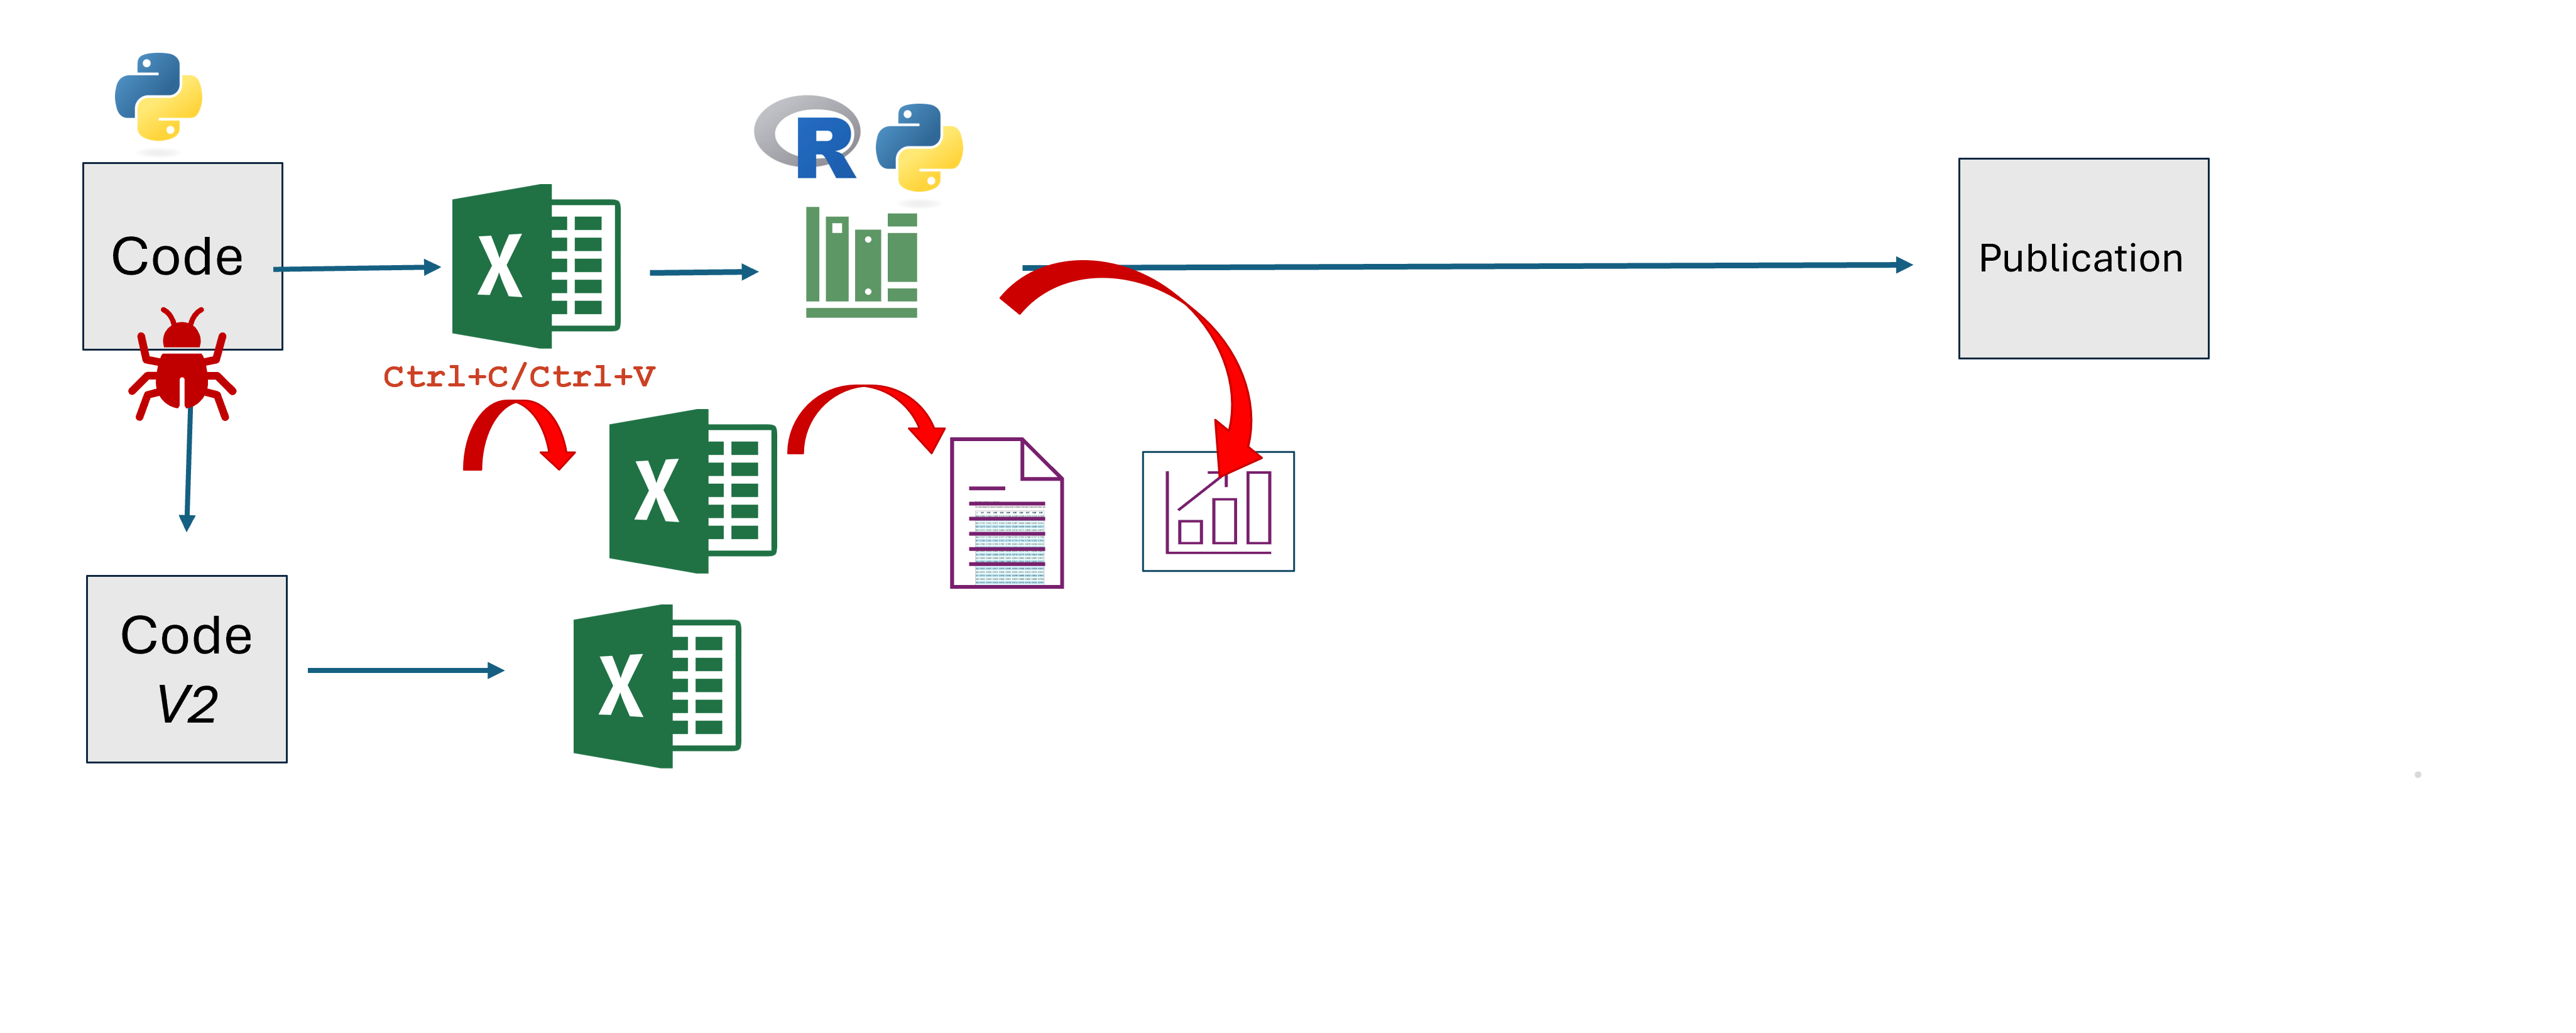
\includegraphics[width=0.8\textwidth]{Process7.png} \\ Comment 7}
        \only<8>{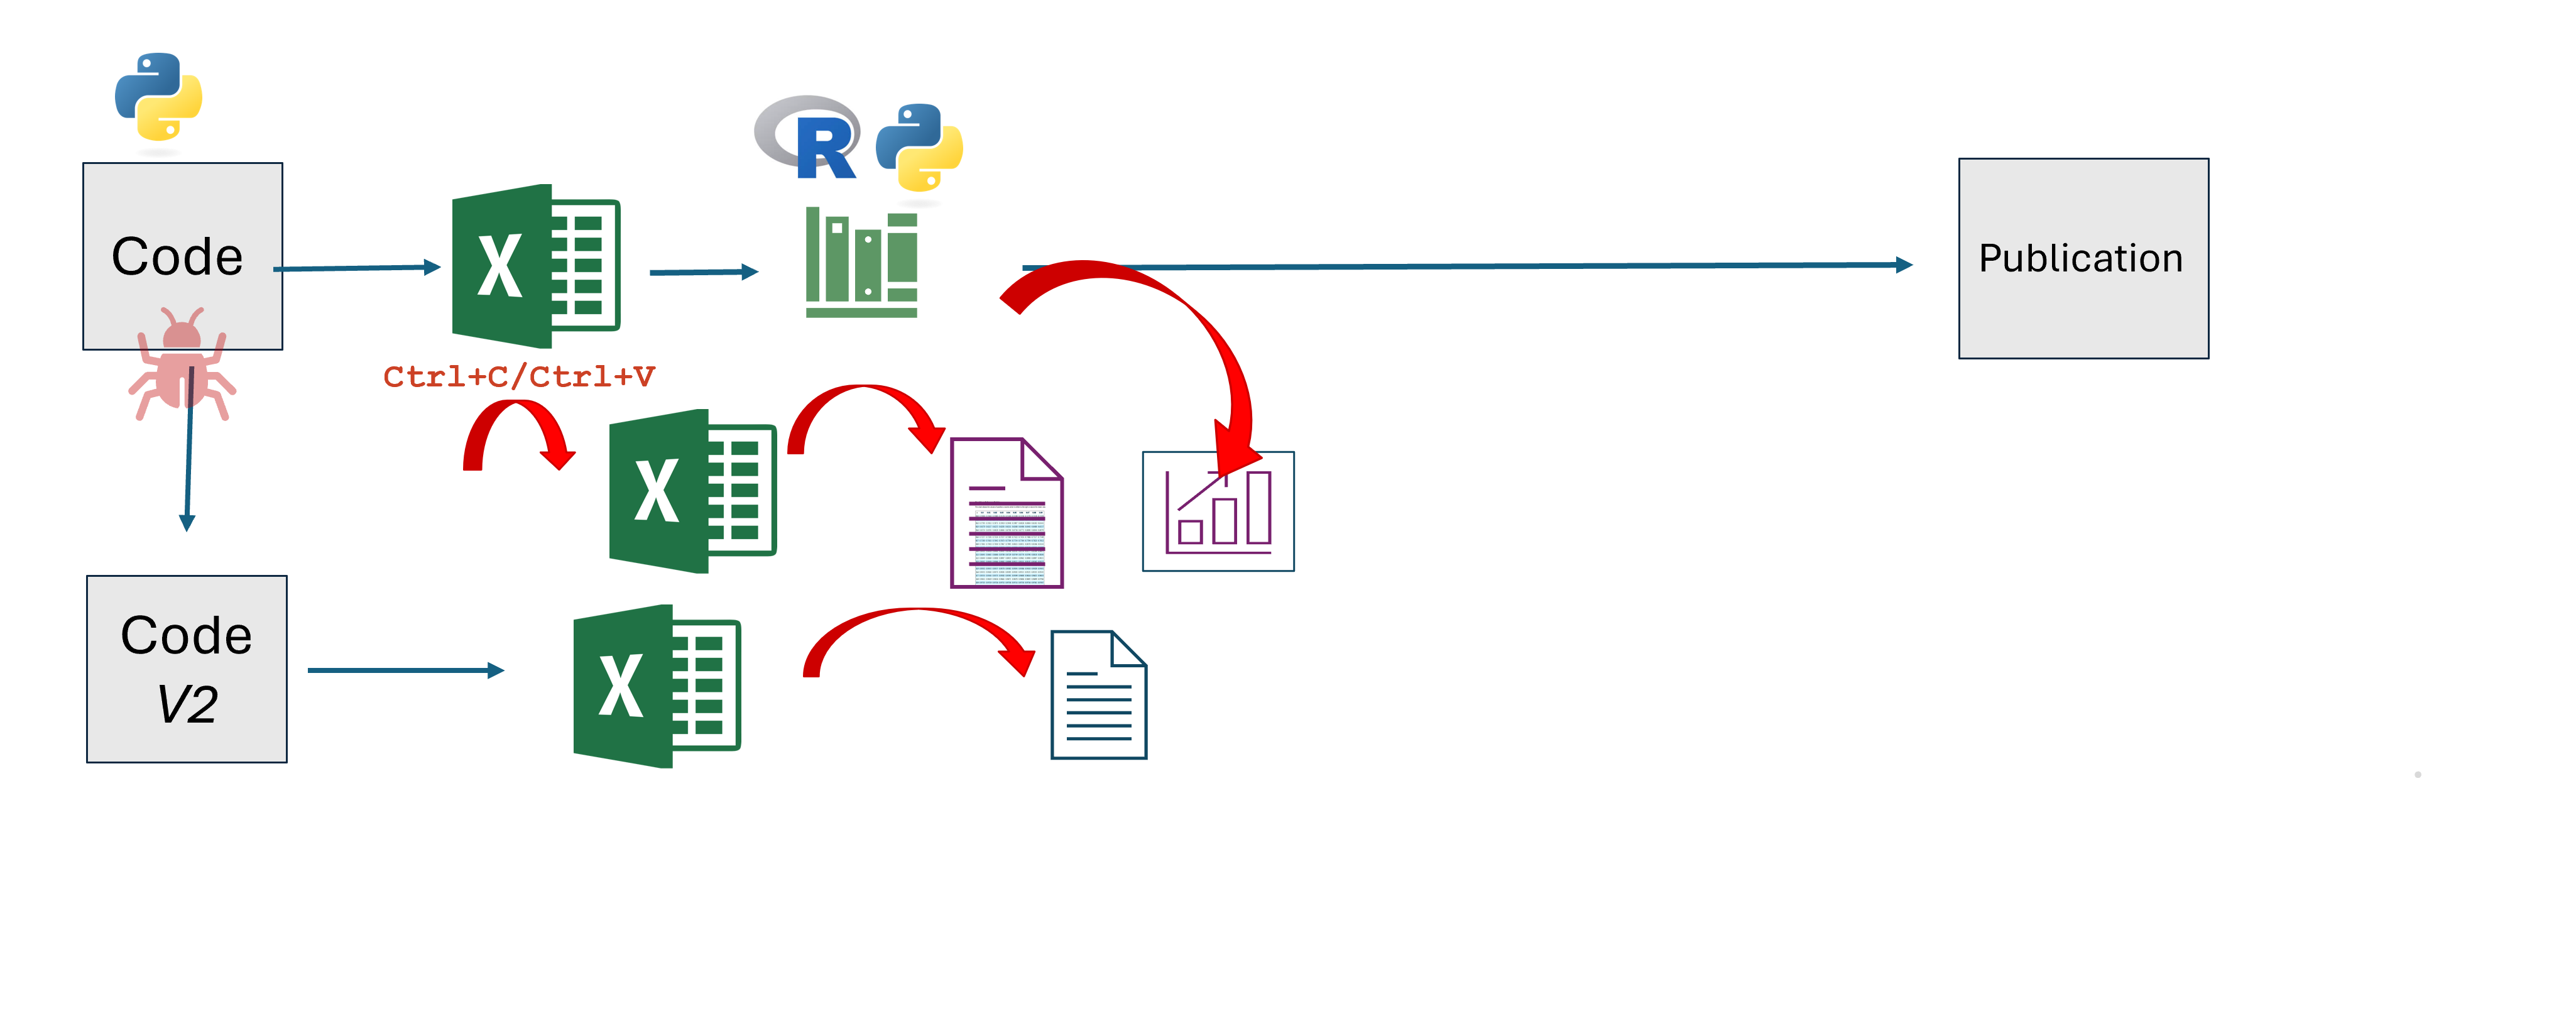
\includegraphics[width=0.8\textwidth]{Process8.png} \\ Comment 8}
        \only<9>{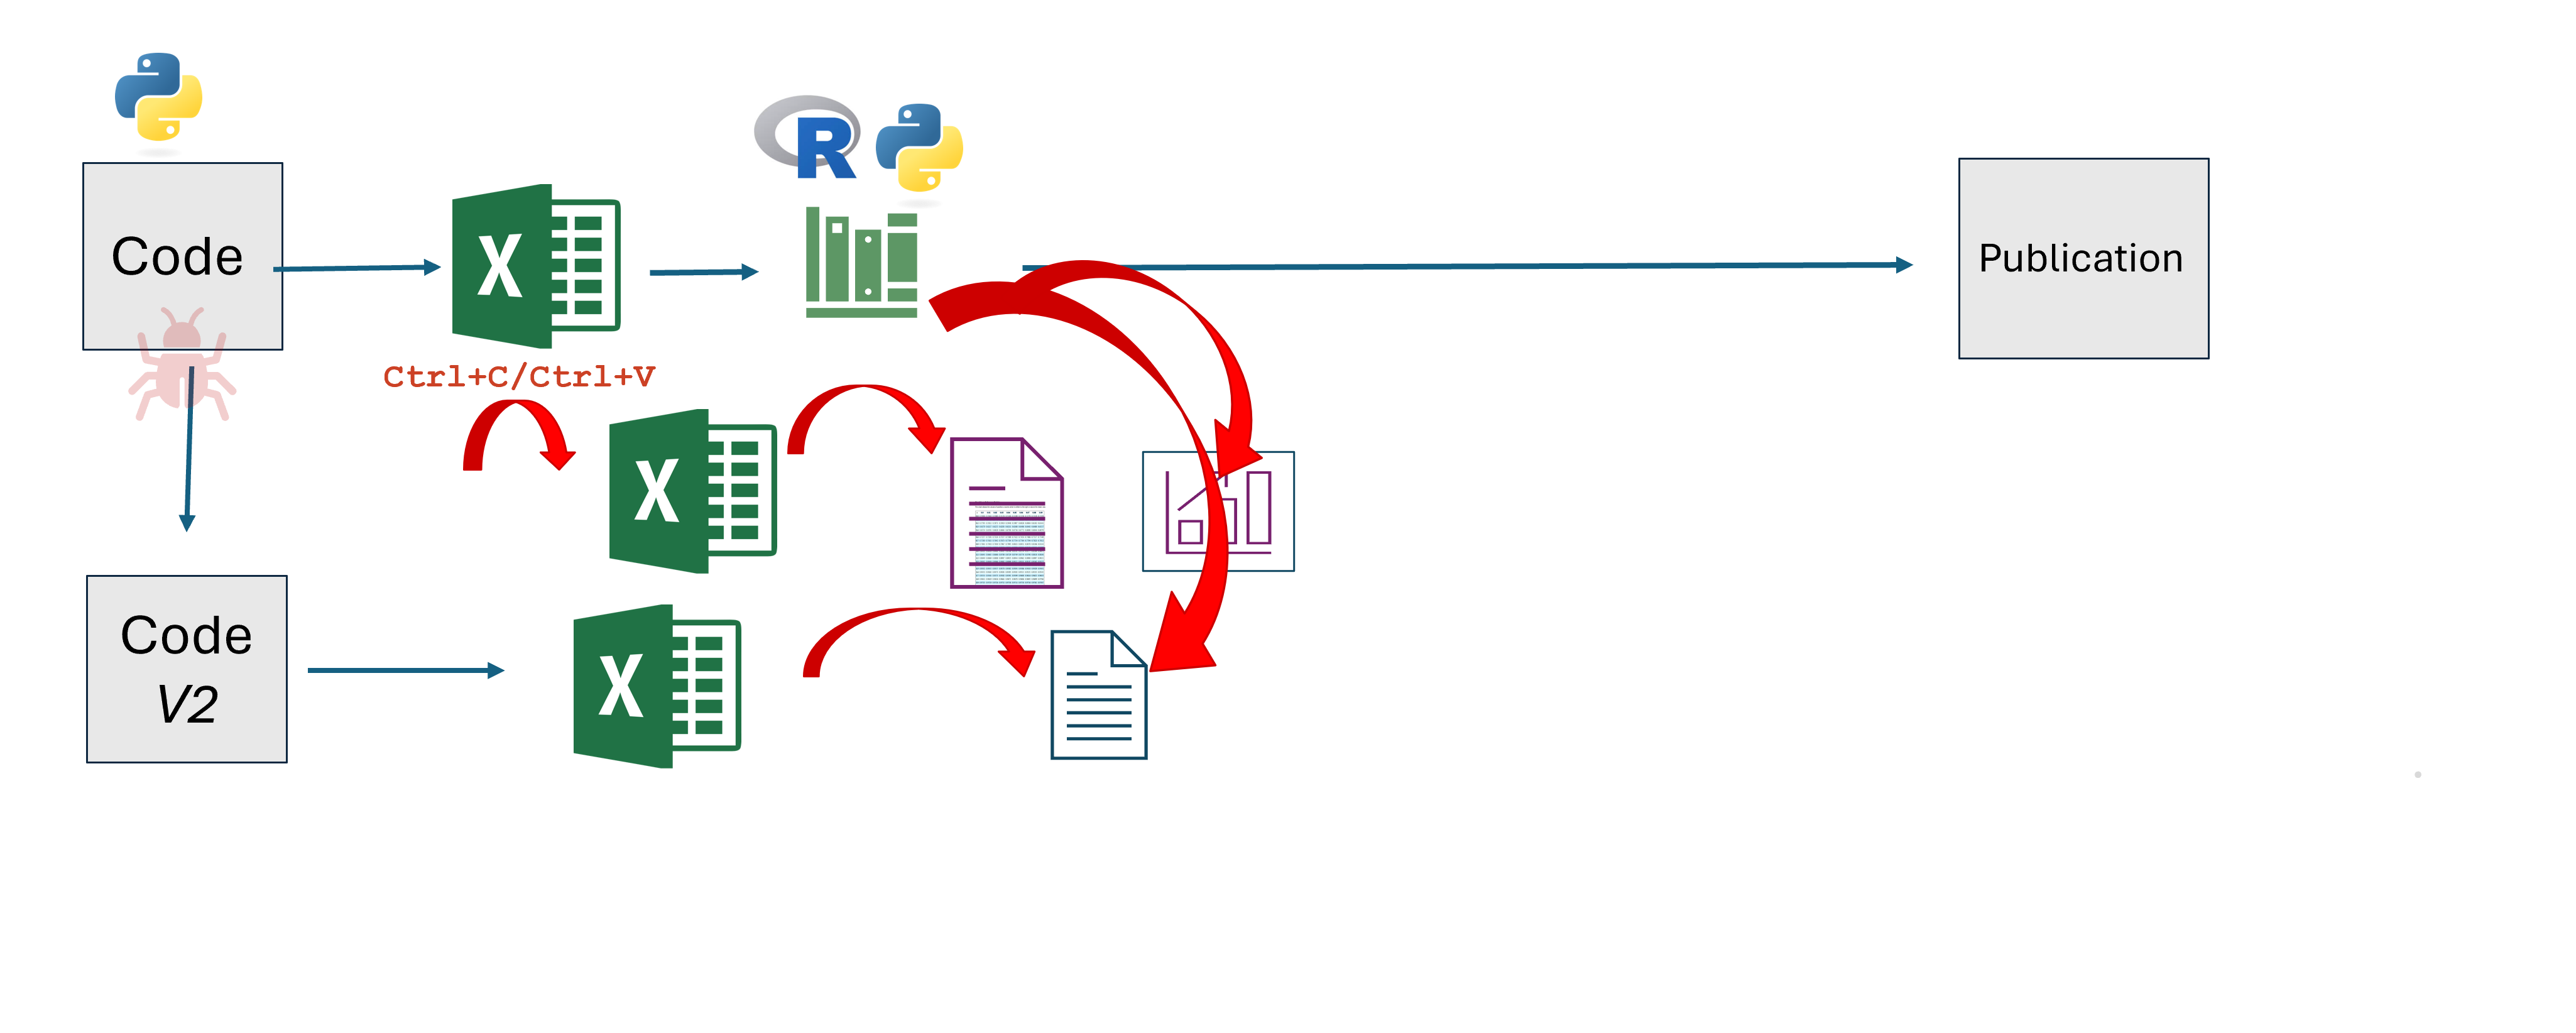
\includegraphics[width=0.8\textwidth]{Process9.png} \\ Comment 9}
        \only<10>{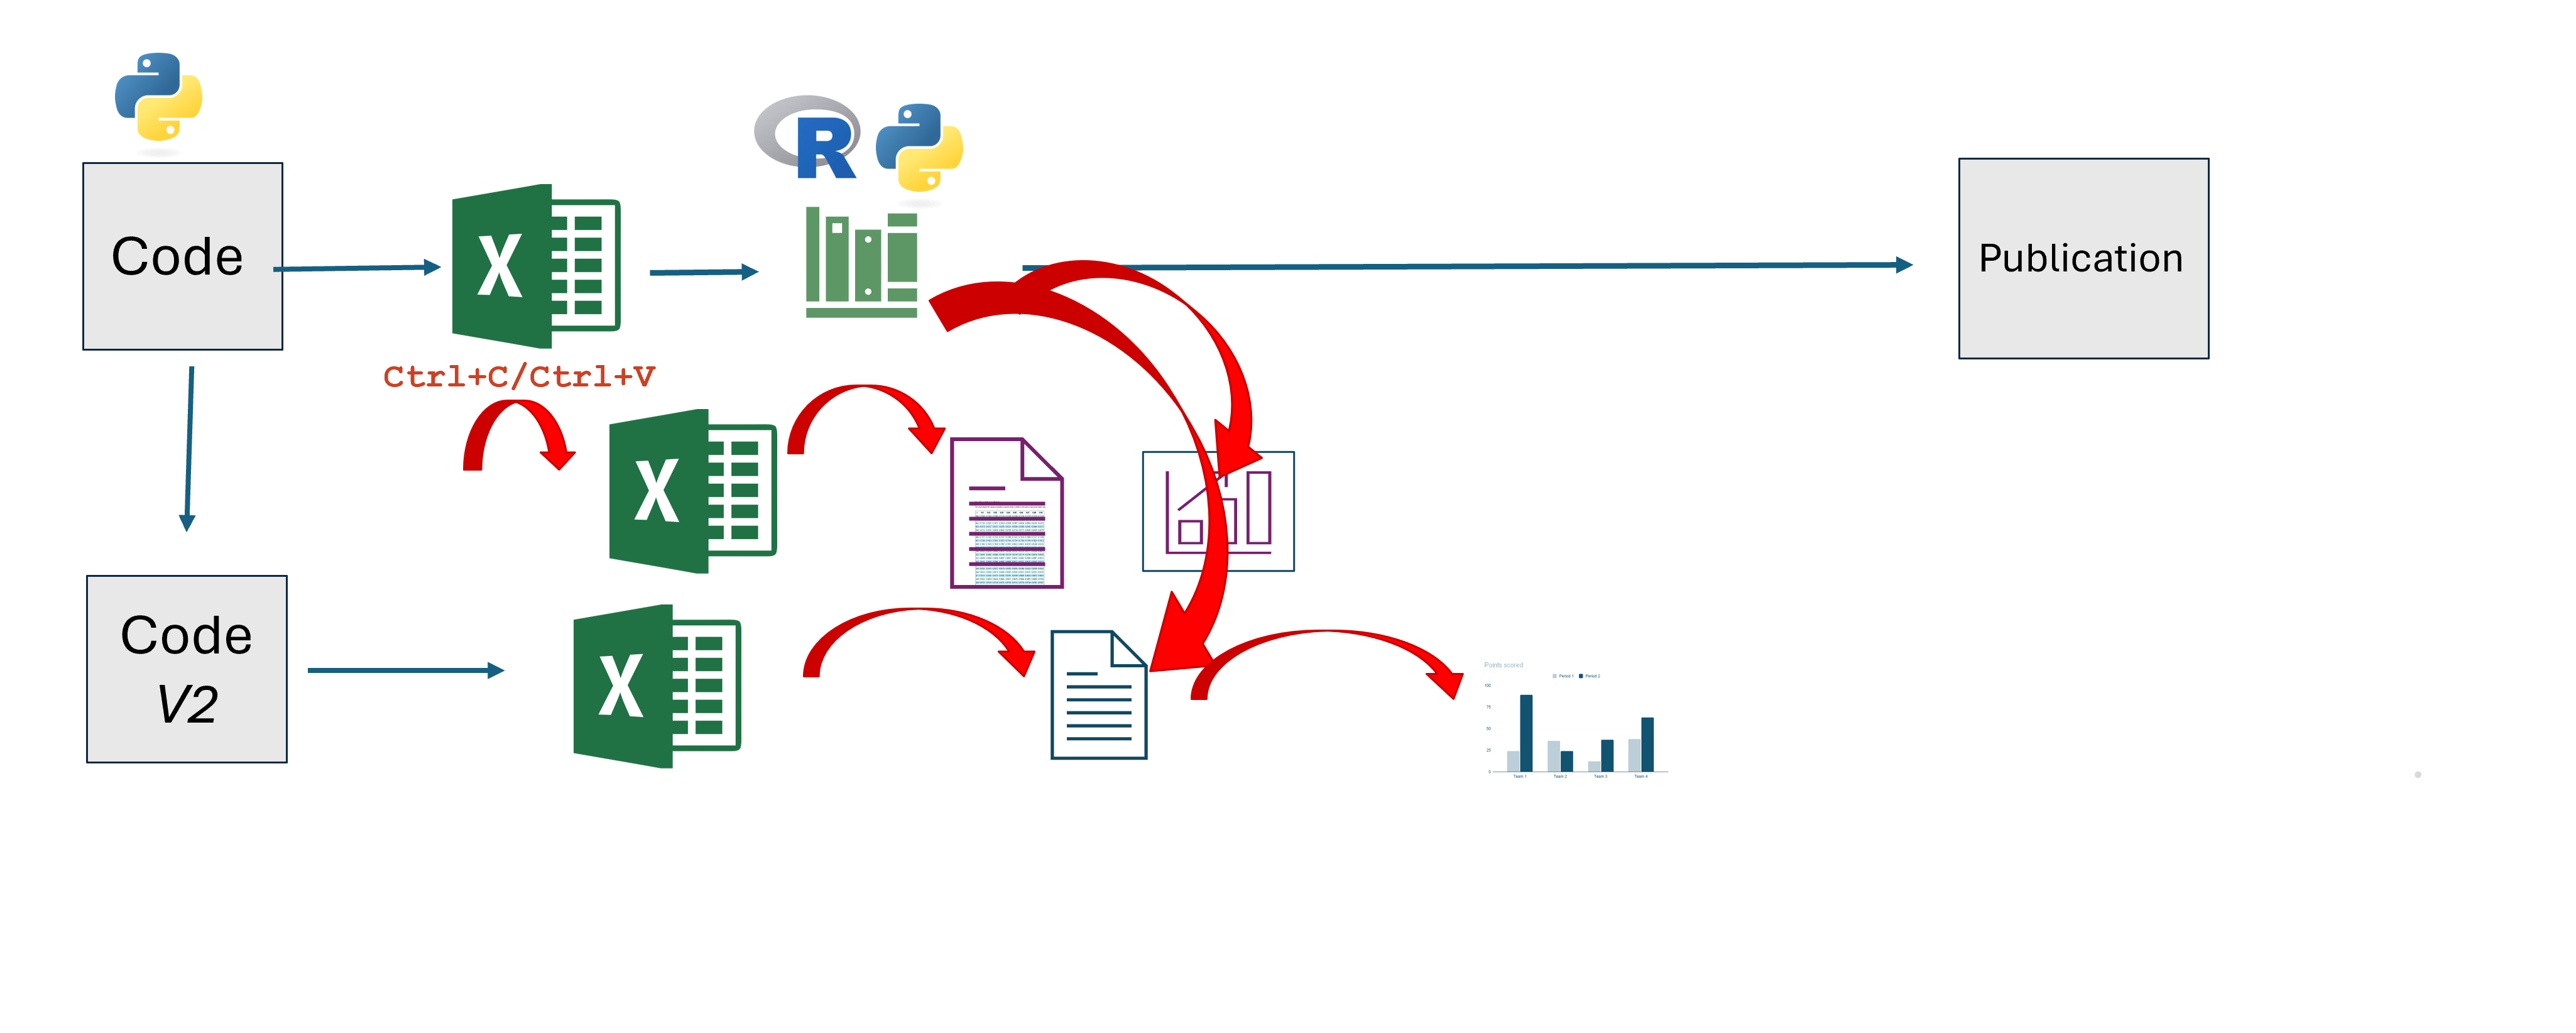
\includegraphics[width=0.8\textwidth]{Process10.png} \\ Comment 10}
        \only<11>{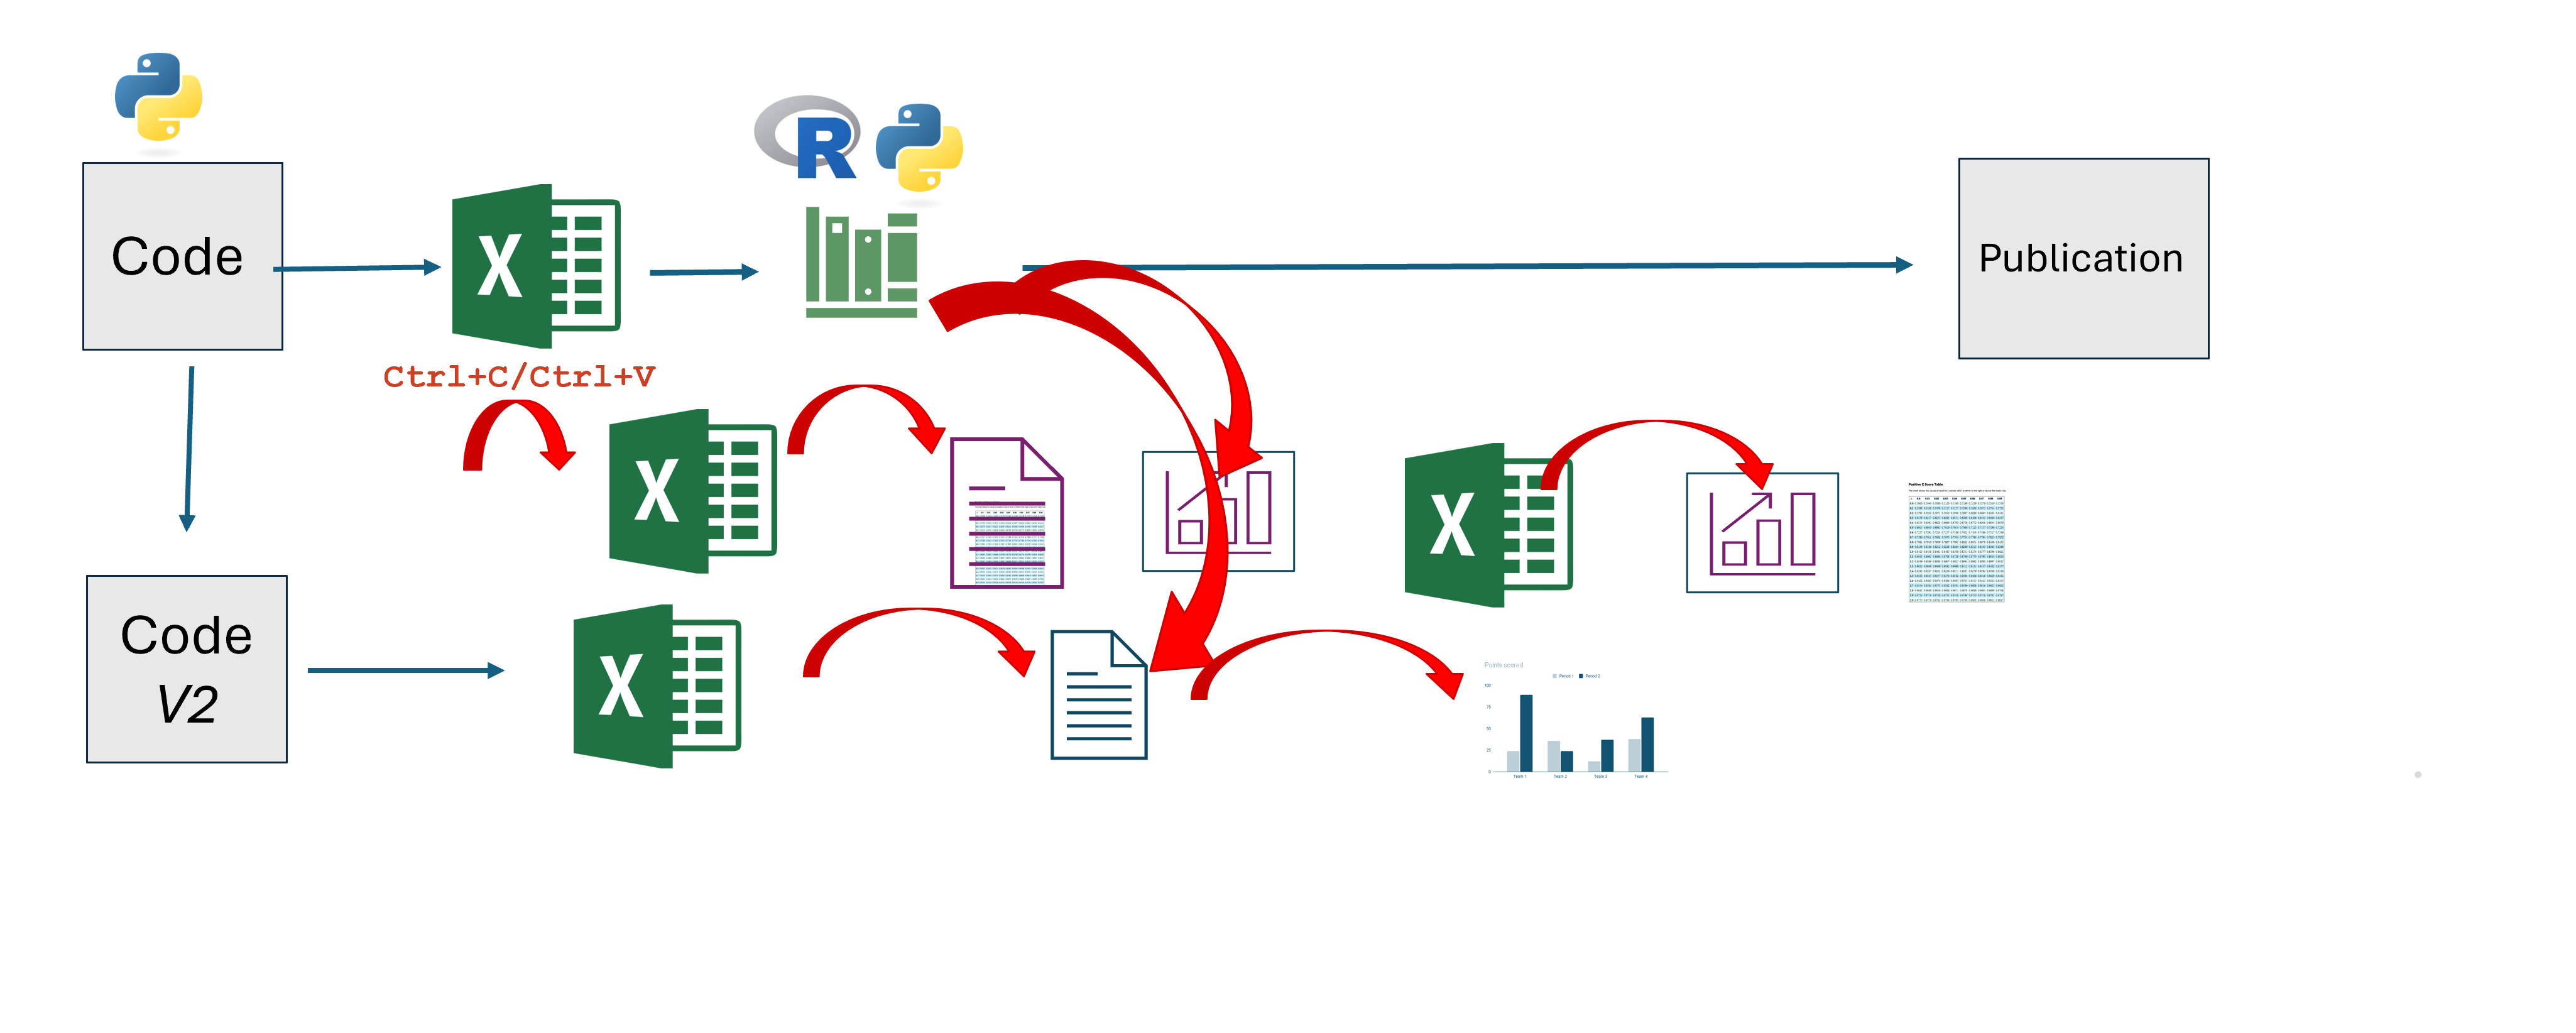
\includegraphics[width=0.8\textwidth]{Process11.png} \\ Comment 9}
        \only<12>{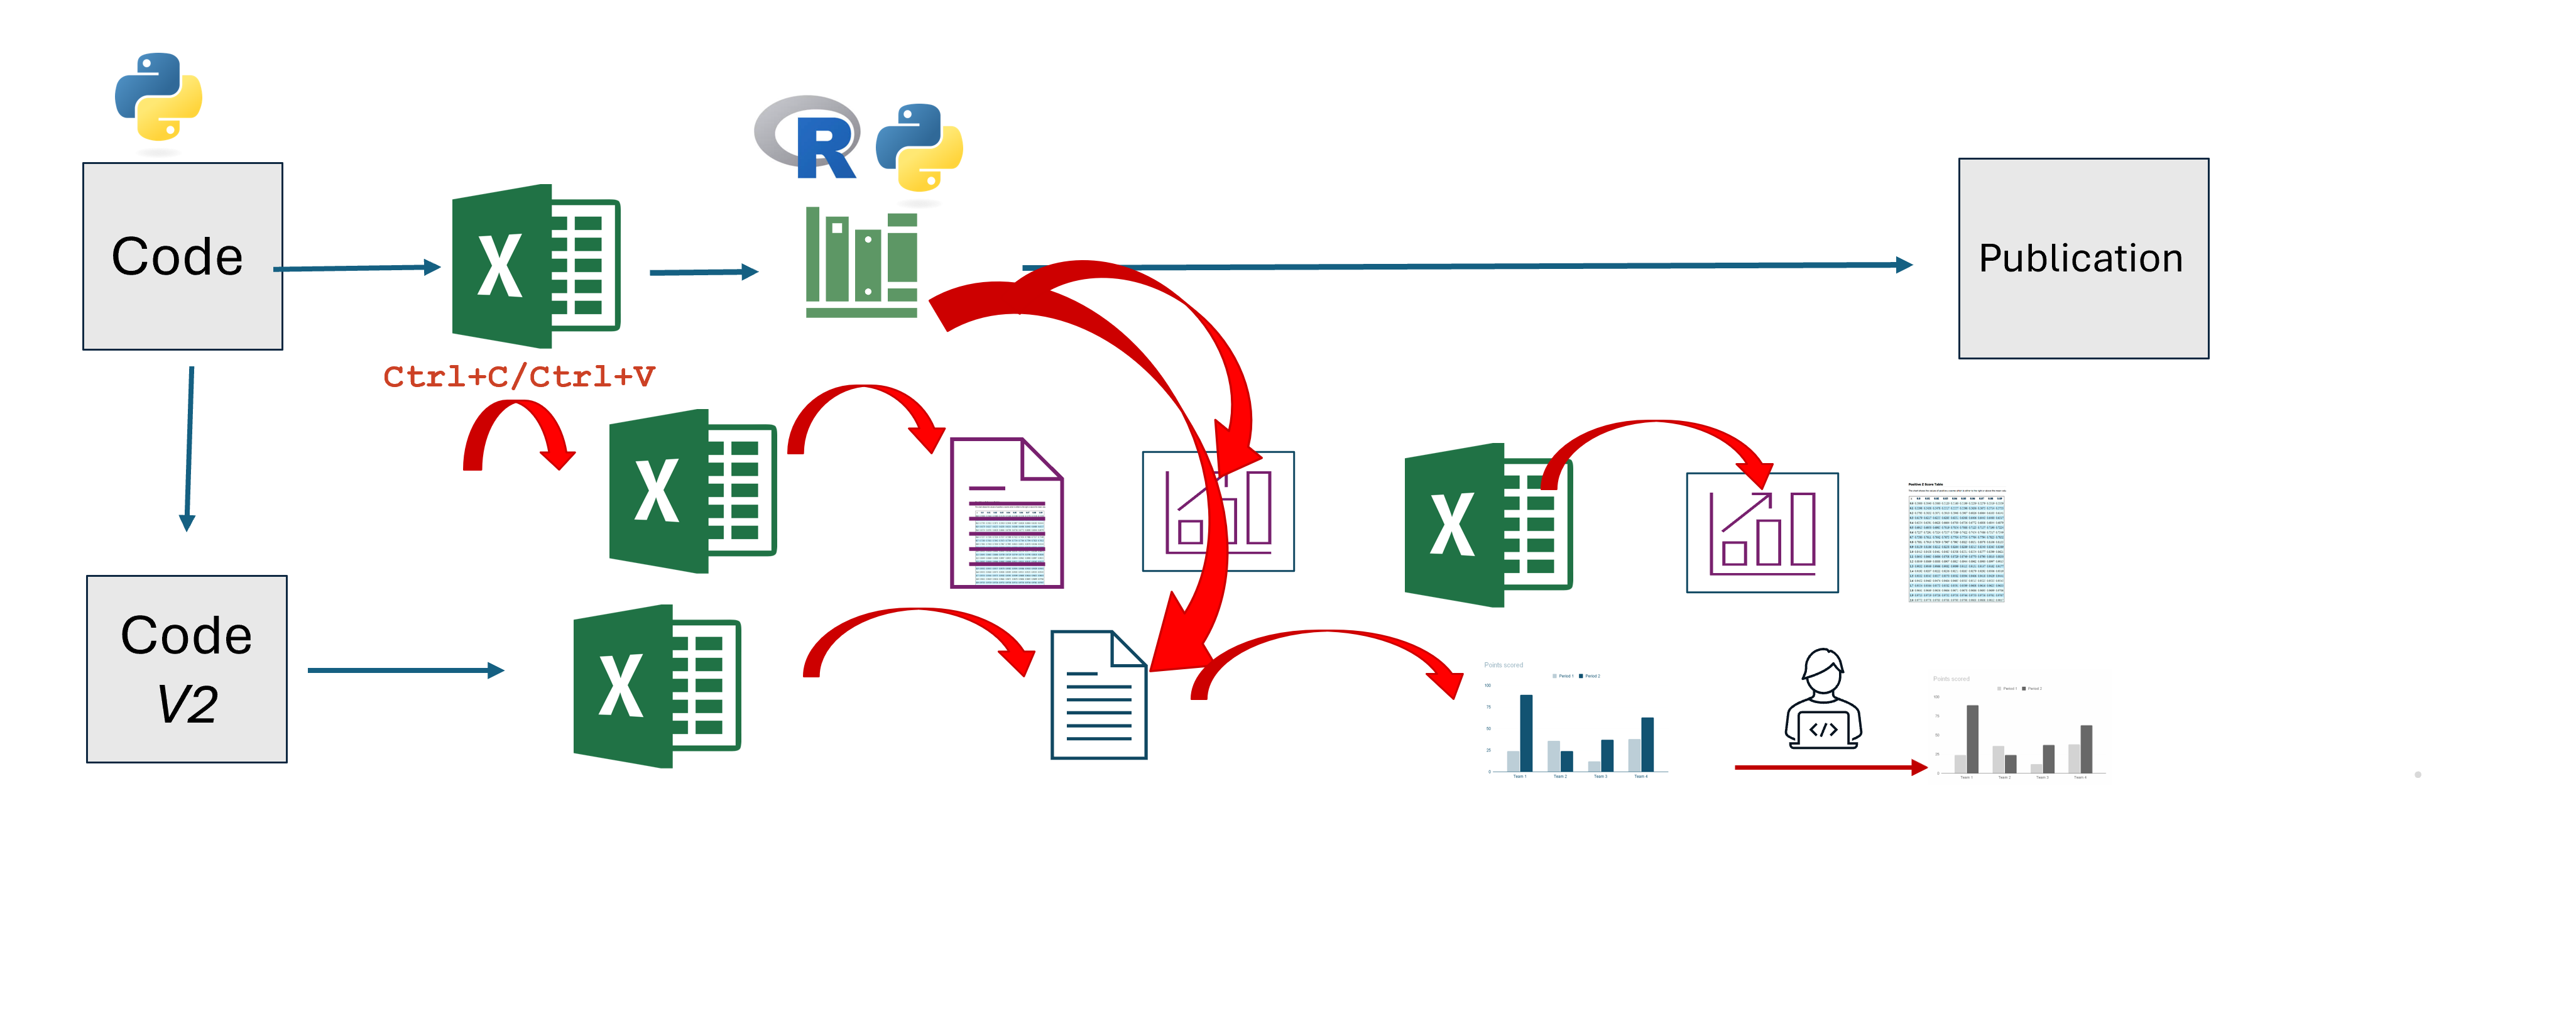
\includegraphics[width=0.8\textwidth]{Process12.png} \\ Comment 10}
        \only<13>{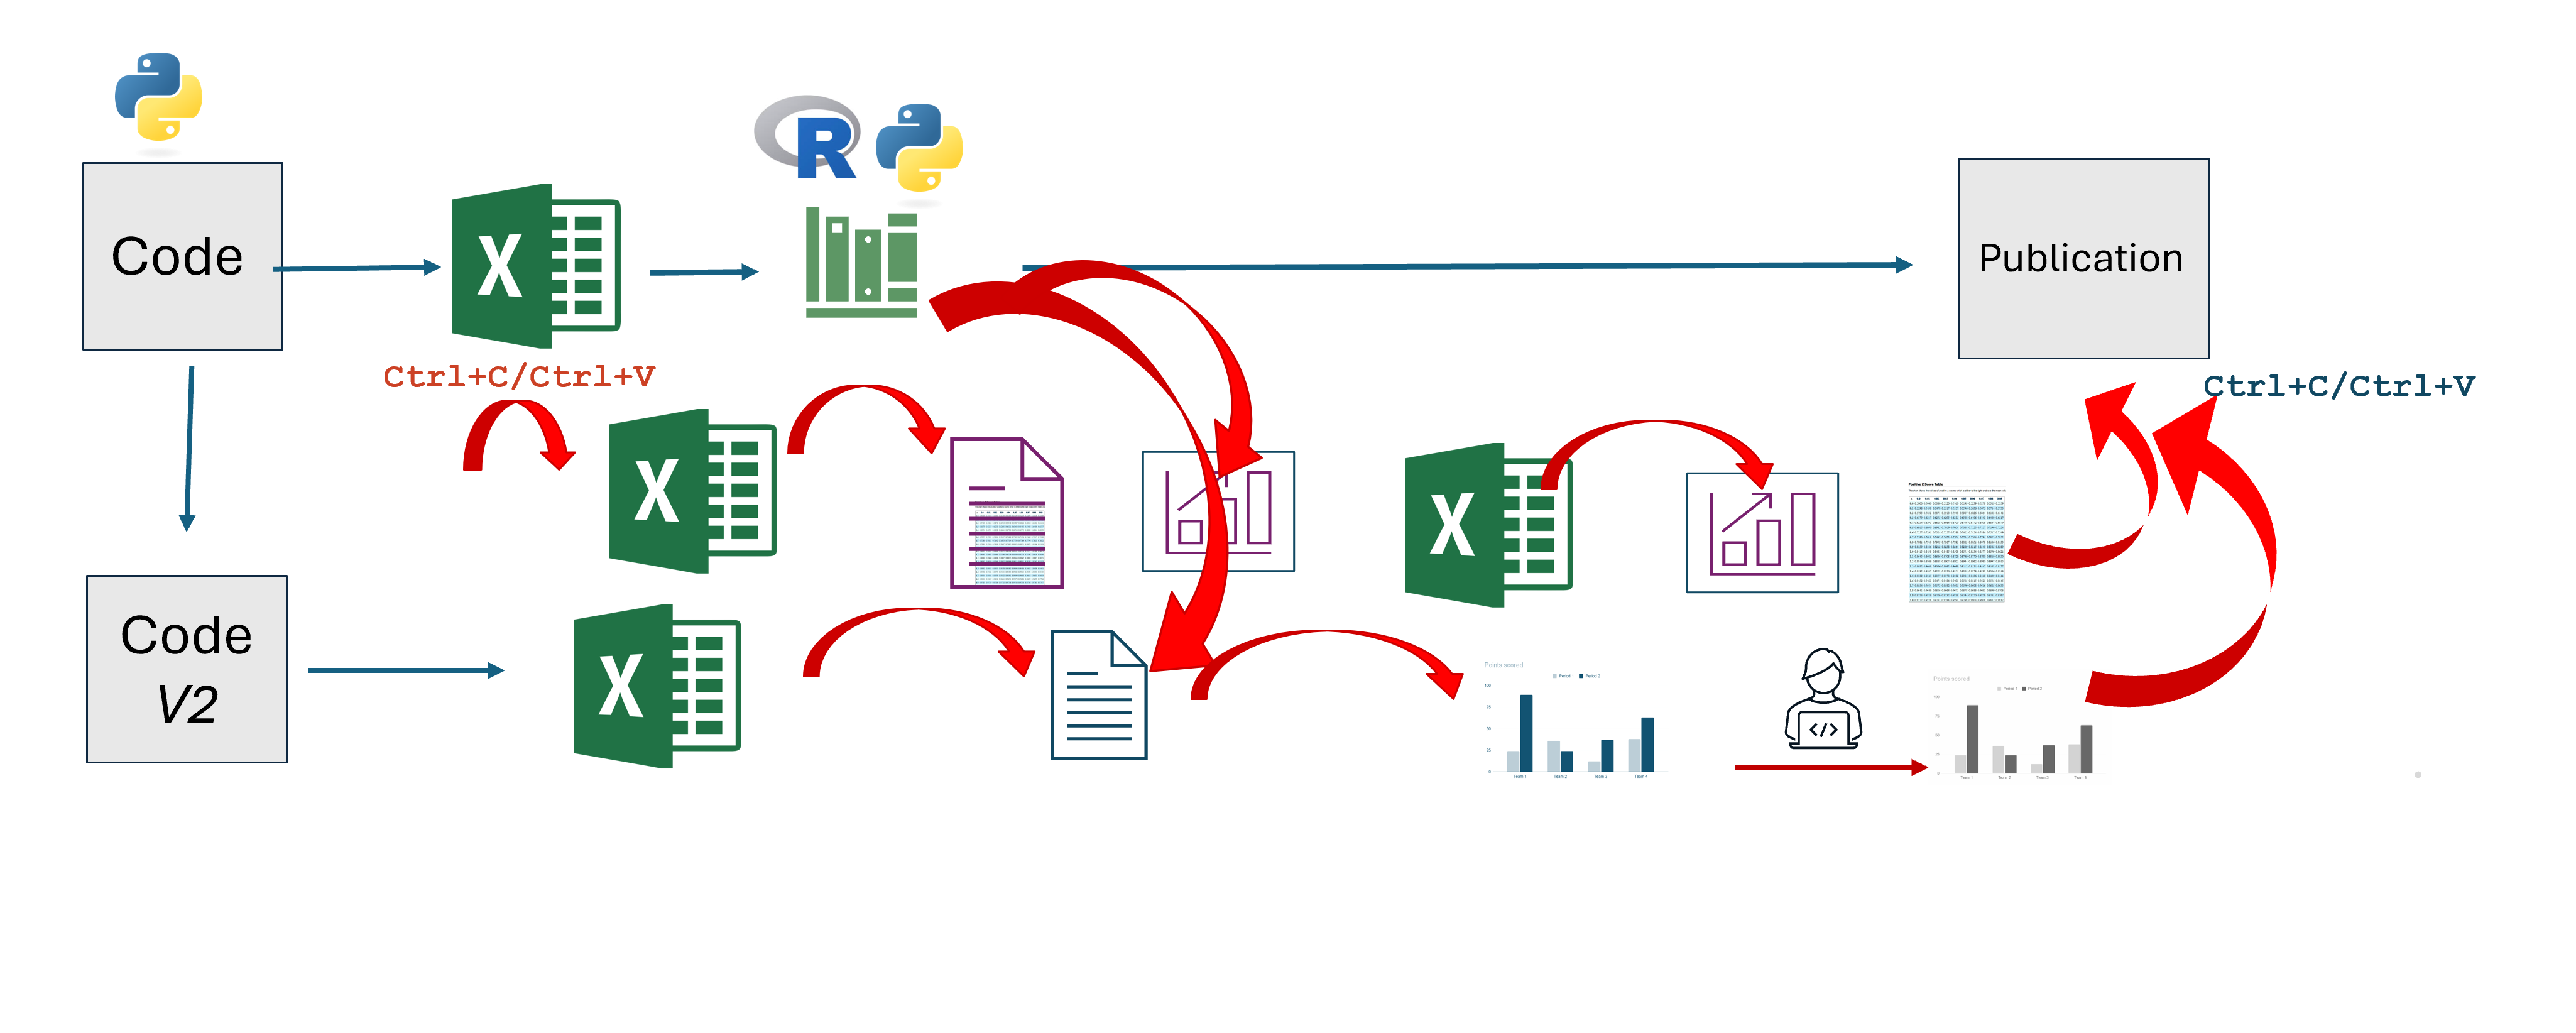
\includegraphics[width=0.8\textwidth]{Process13.png} \\ Comment 9}
        \only<14>{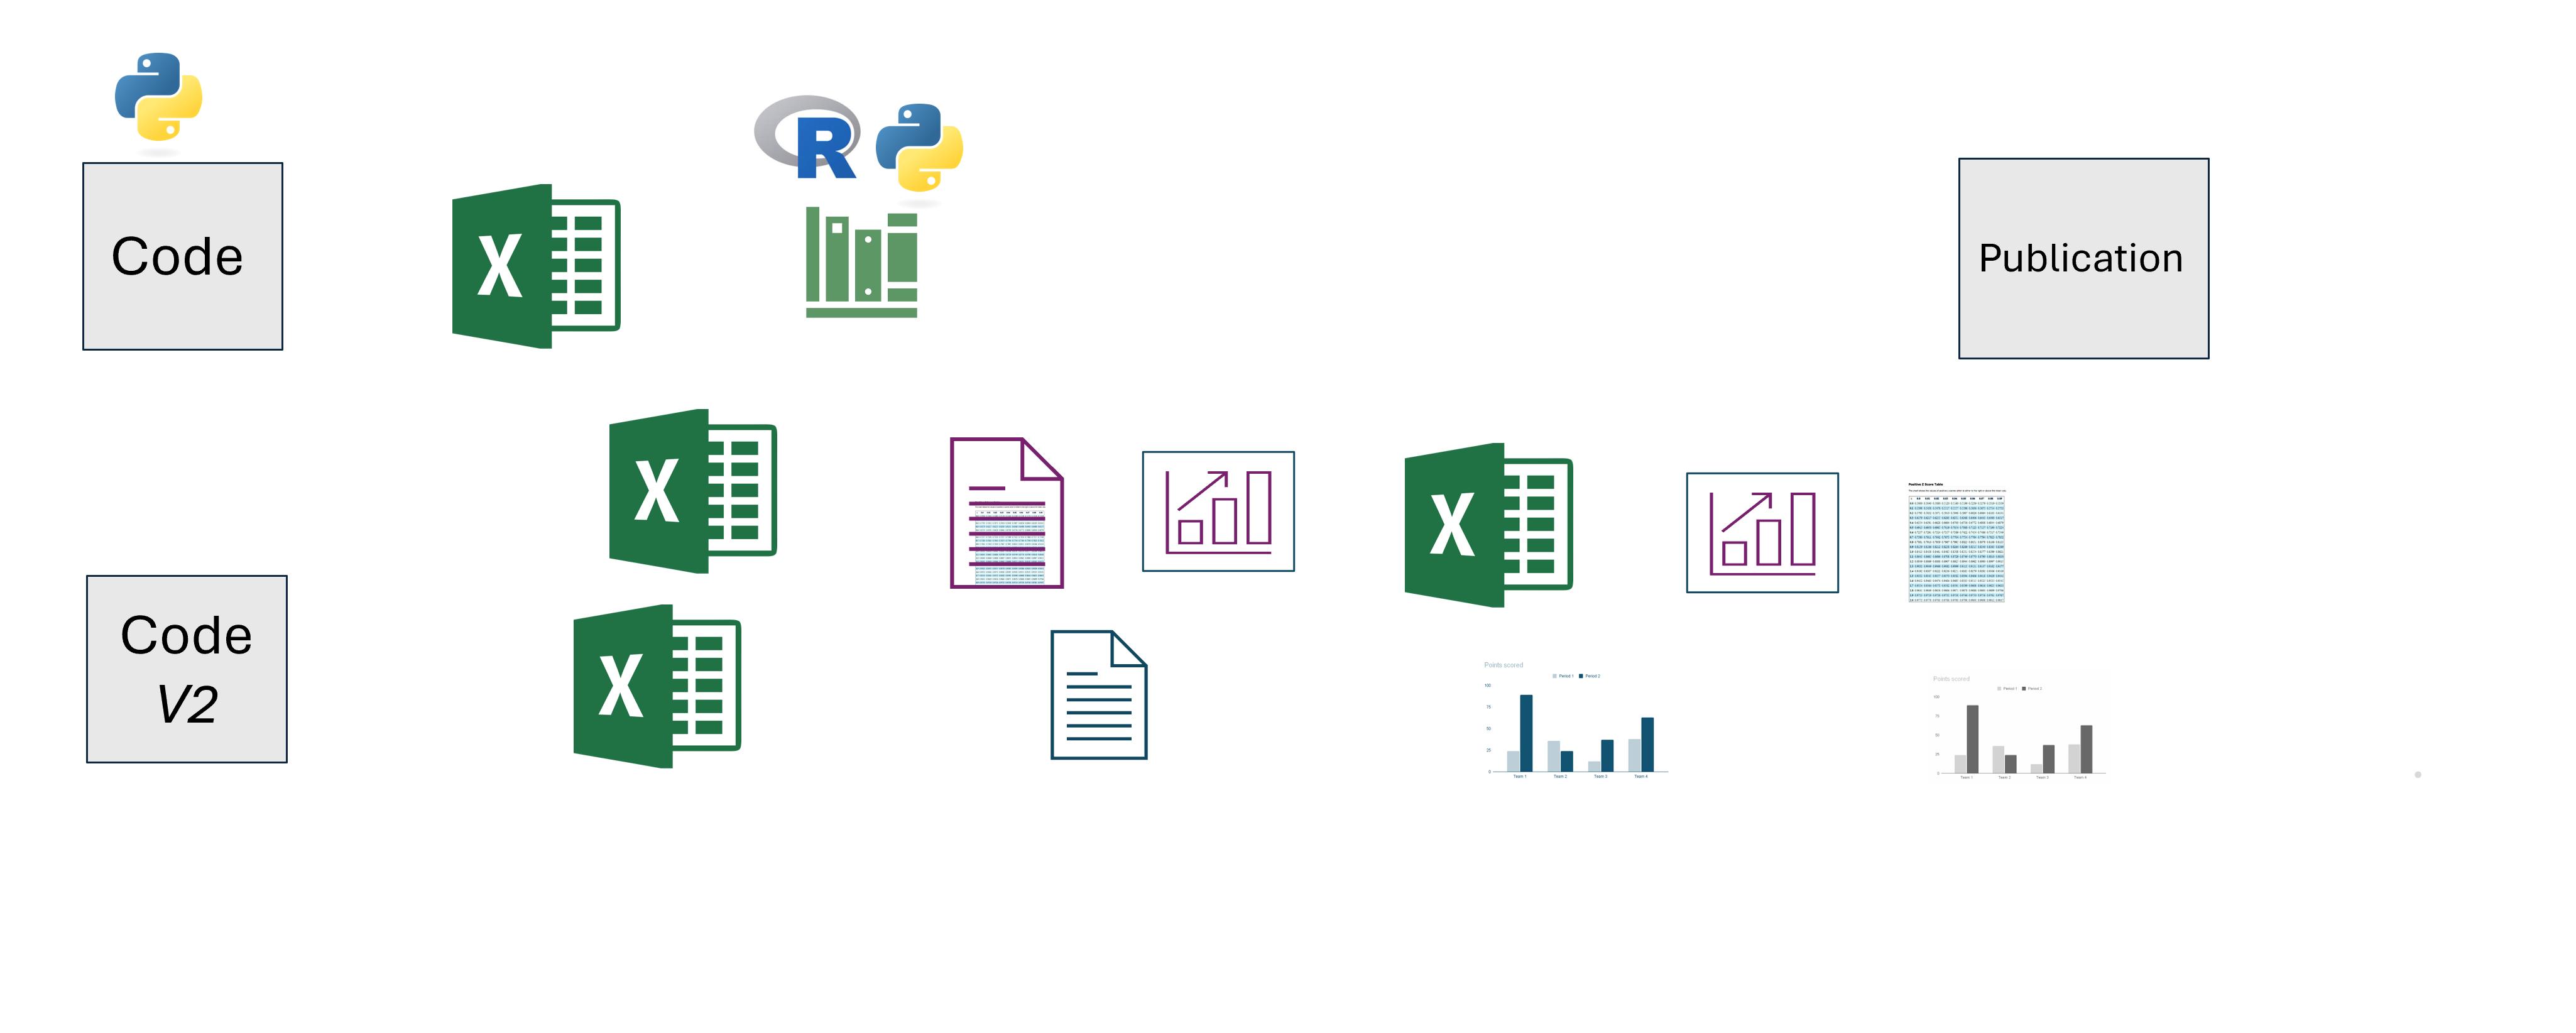
\includegraphics[width=0.8\textwidth]{Process14.png} \\ Comment 10}
    \end{itemize}
\end{center}
\end{frame}


\begin{frame}{Usual practice: In the end}

 \begin{columns}[T]
    \begin{column}{0.5\textwidth}
      \begin{itemize}[<+->]
        \item Lots of files
        \item Cut and paste is not a reliable, reproducible approach!
        \item Your brain may remember..
        \item[] ...all the steps...
        \item[] .. in the right order..
        \item[]...all of them !
        \item Or use (bad) "\emph{tools}"
      \end{itemize}
    \end{column}
    \begin{column}{0.5\textwidth}
       \begin{itemize}
       \item[] \only<1>{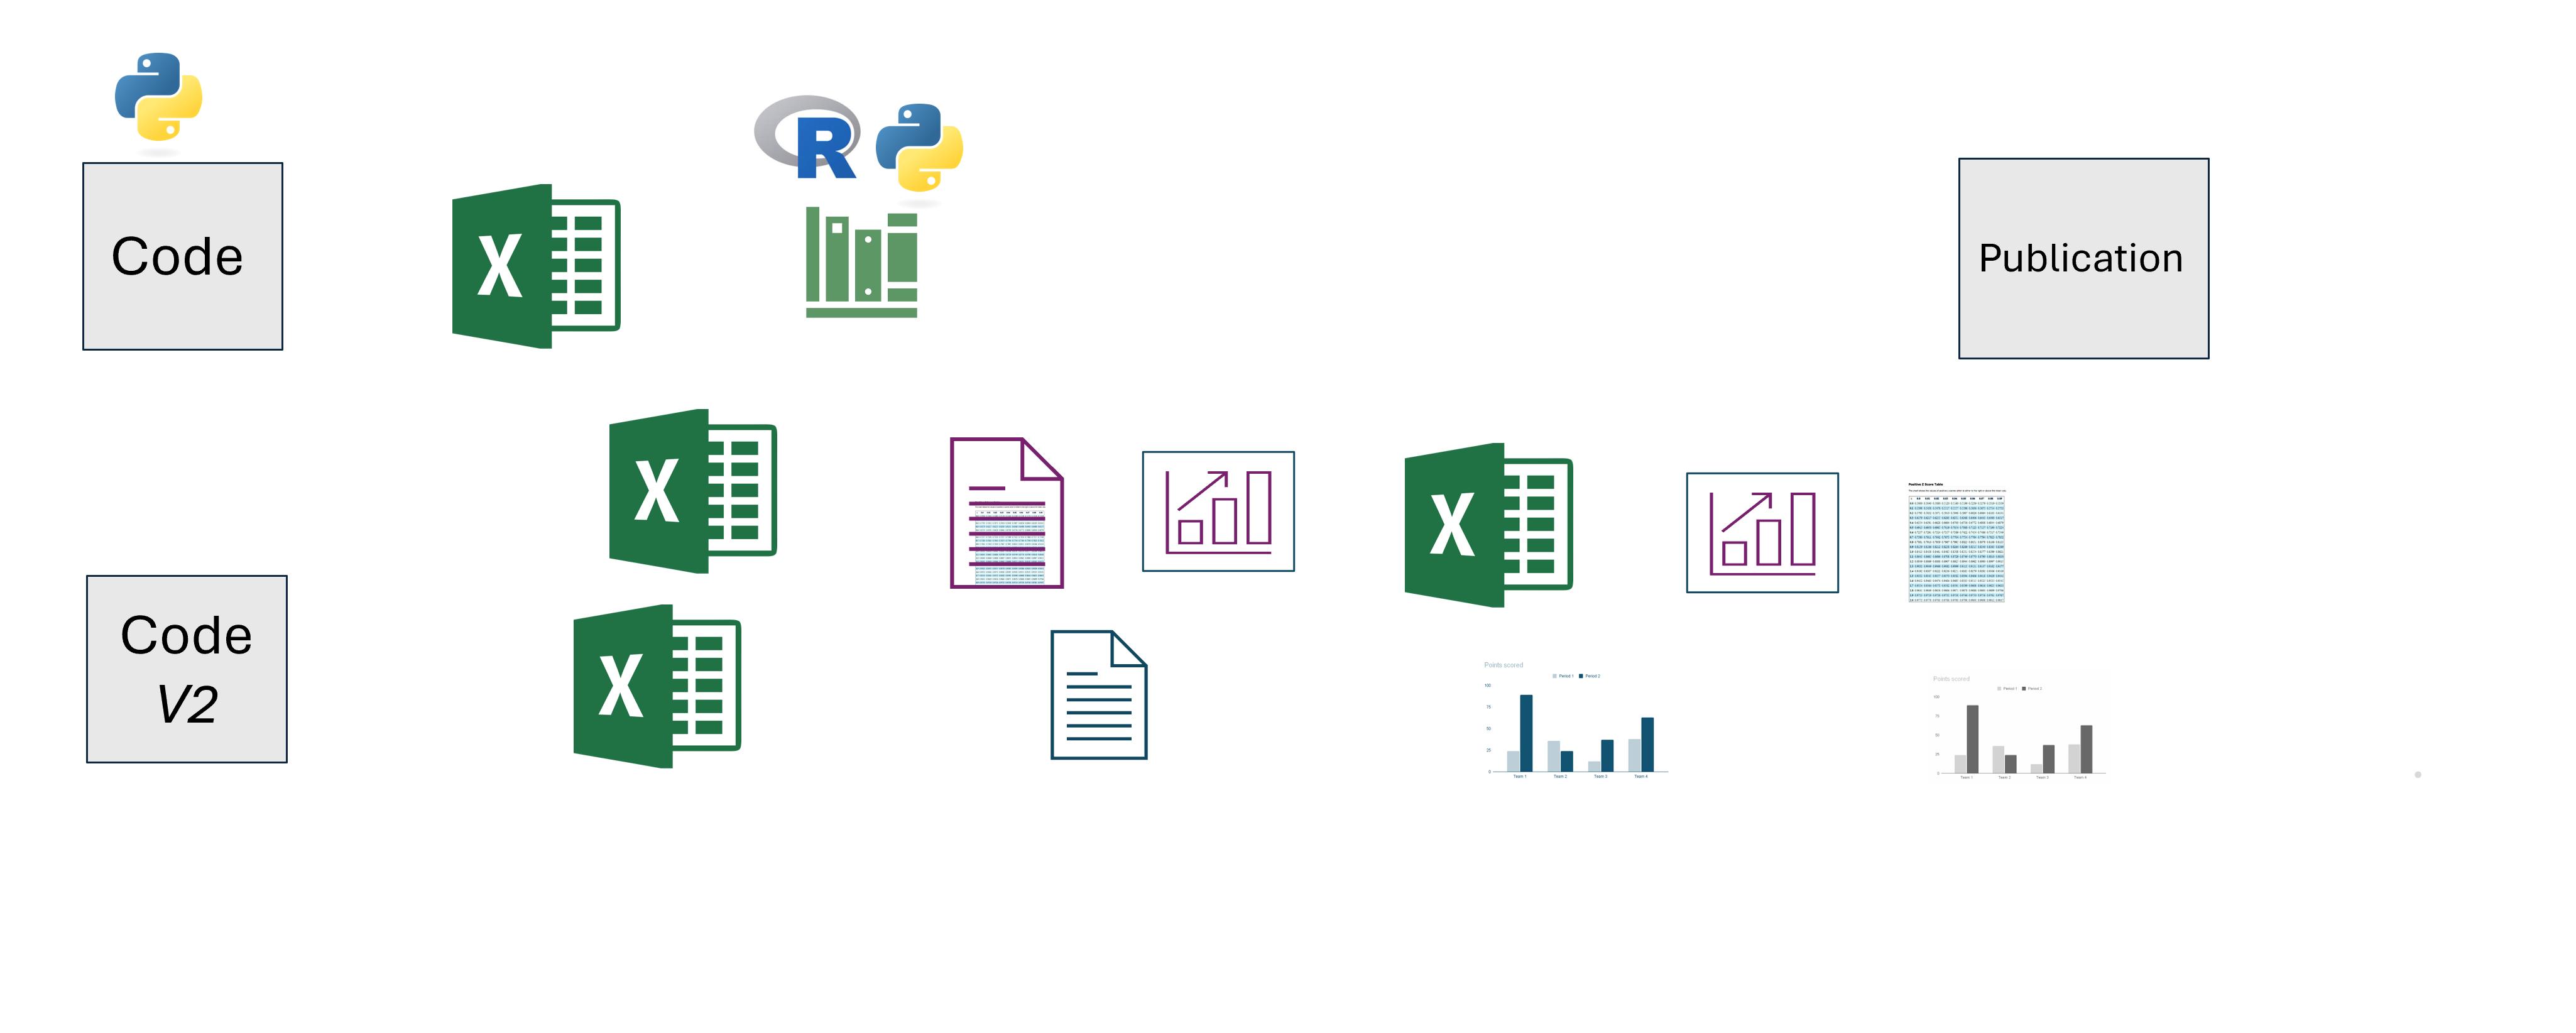
\includegraphics[width=0.8\textwidth]{Process14.png} }
        \only<2>{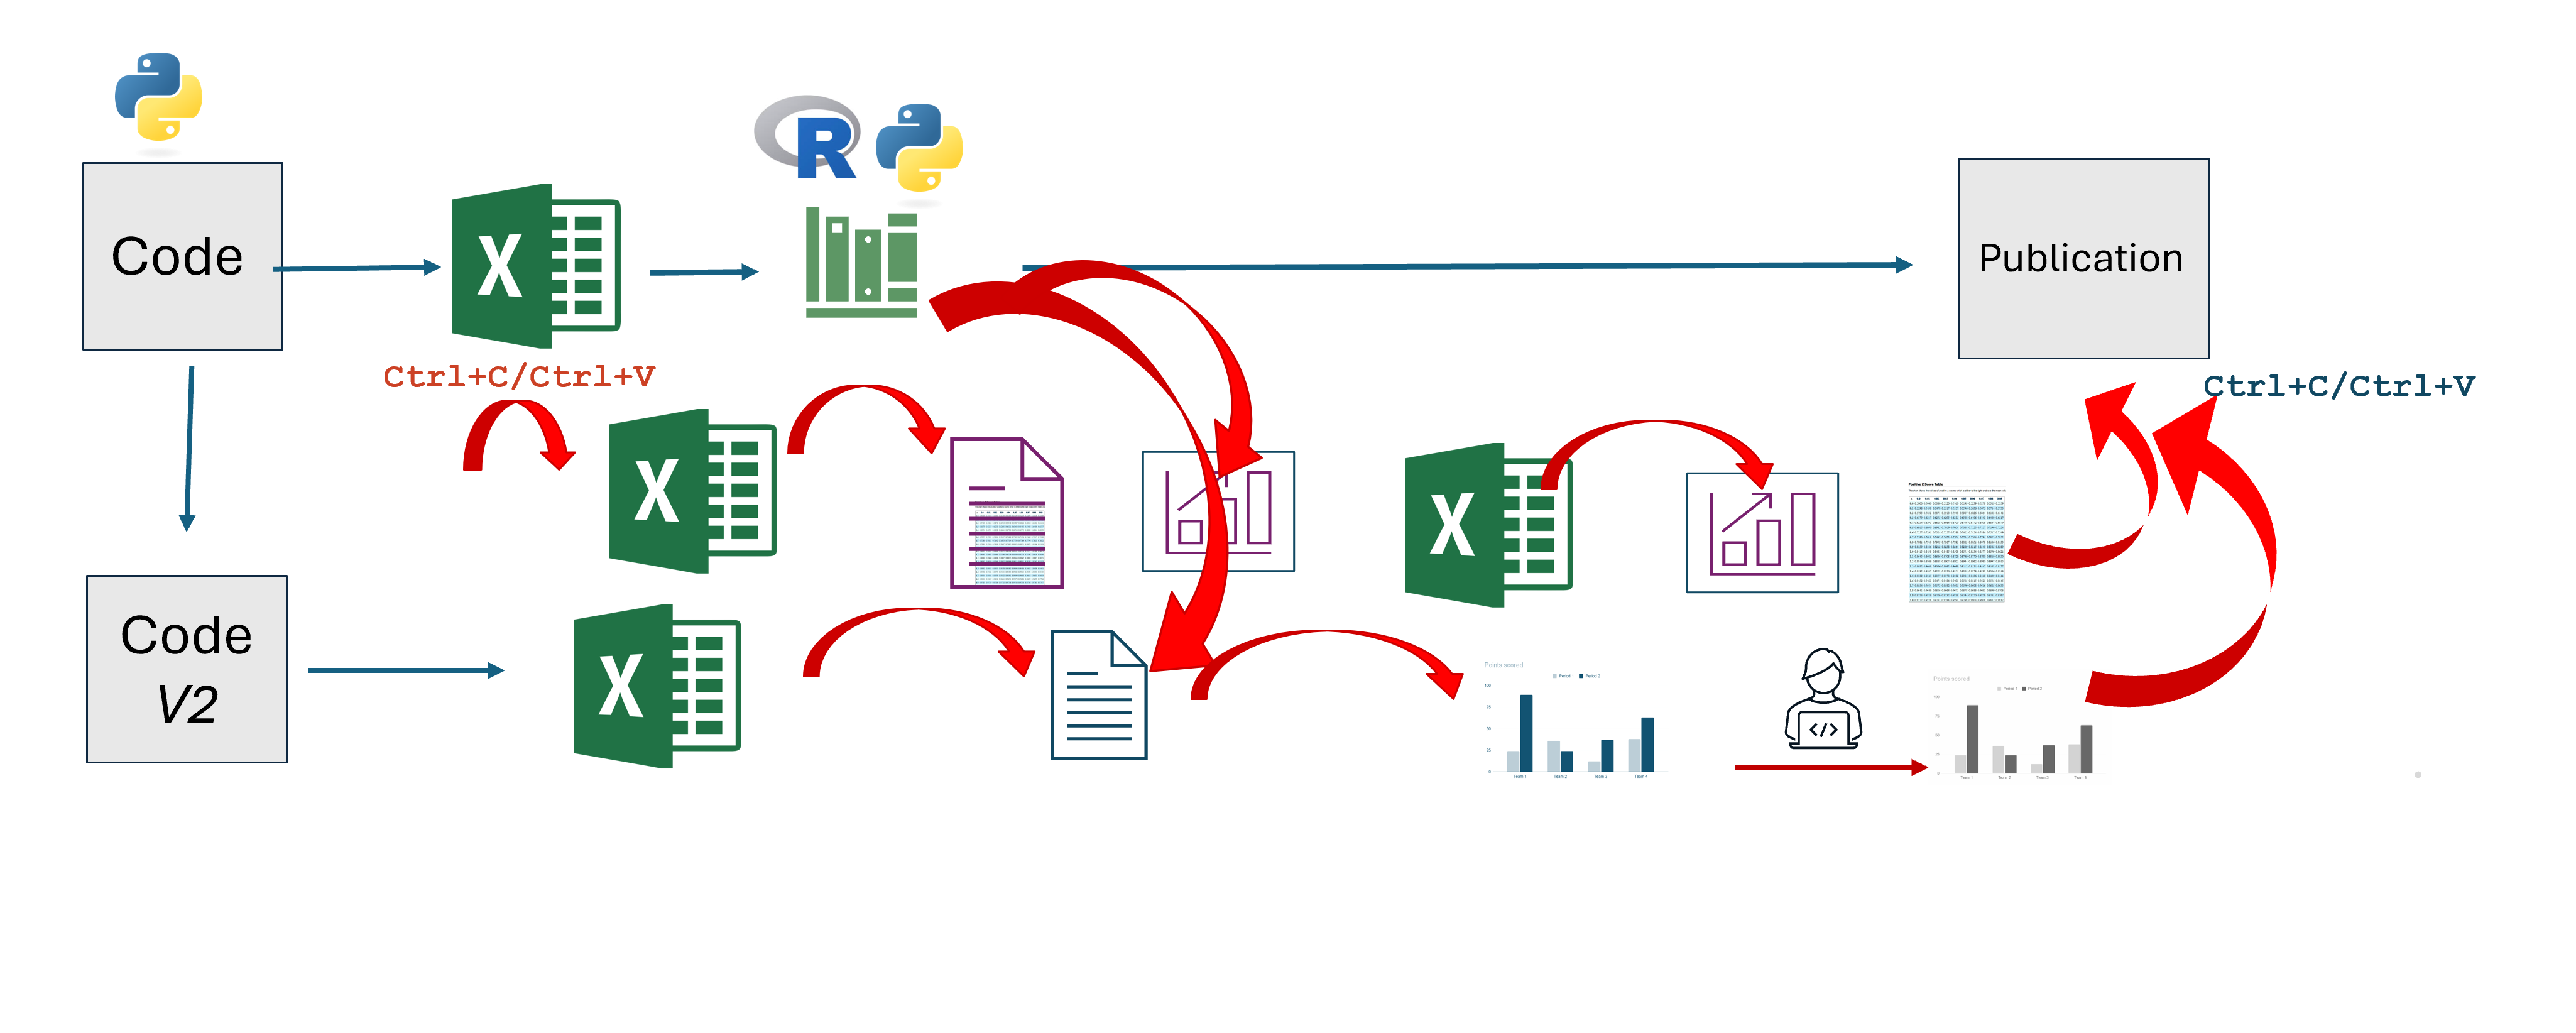
\includegraphics[width=1.0\textwidth]{Process13.png} }
        \only<3>{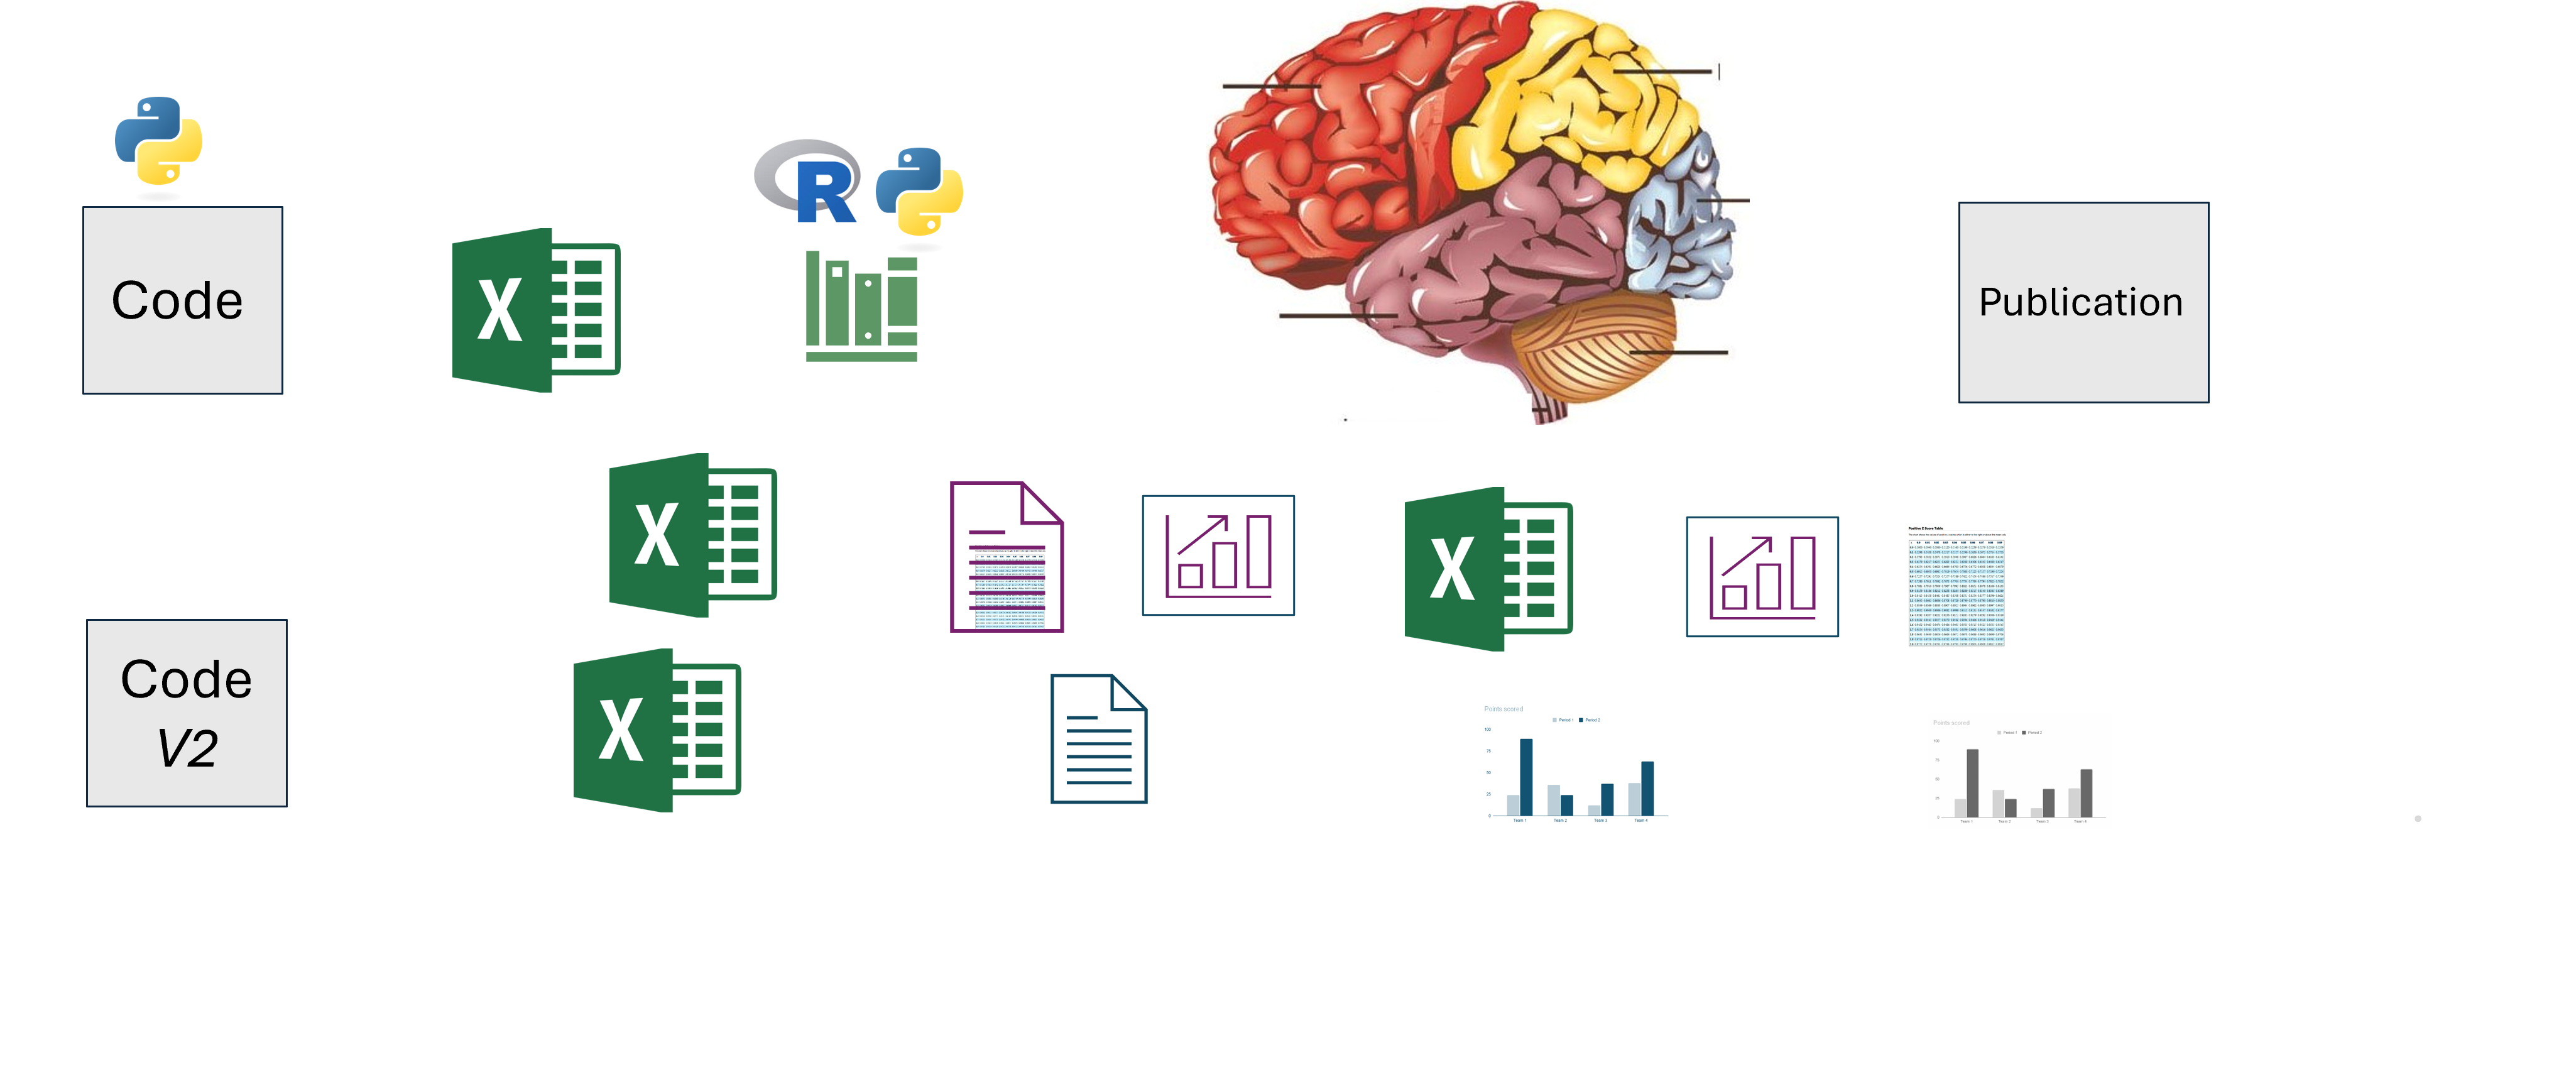
\includegraphics[width=1.0\textwidth]{Process15.png} }
        \only<4>{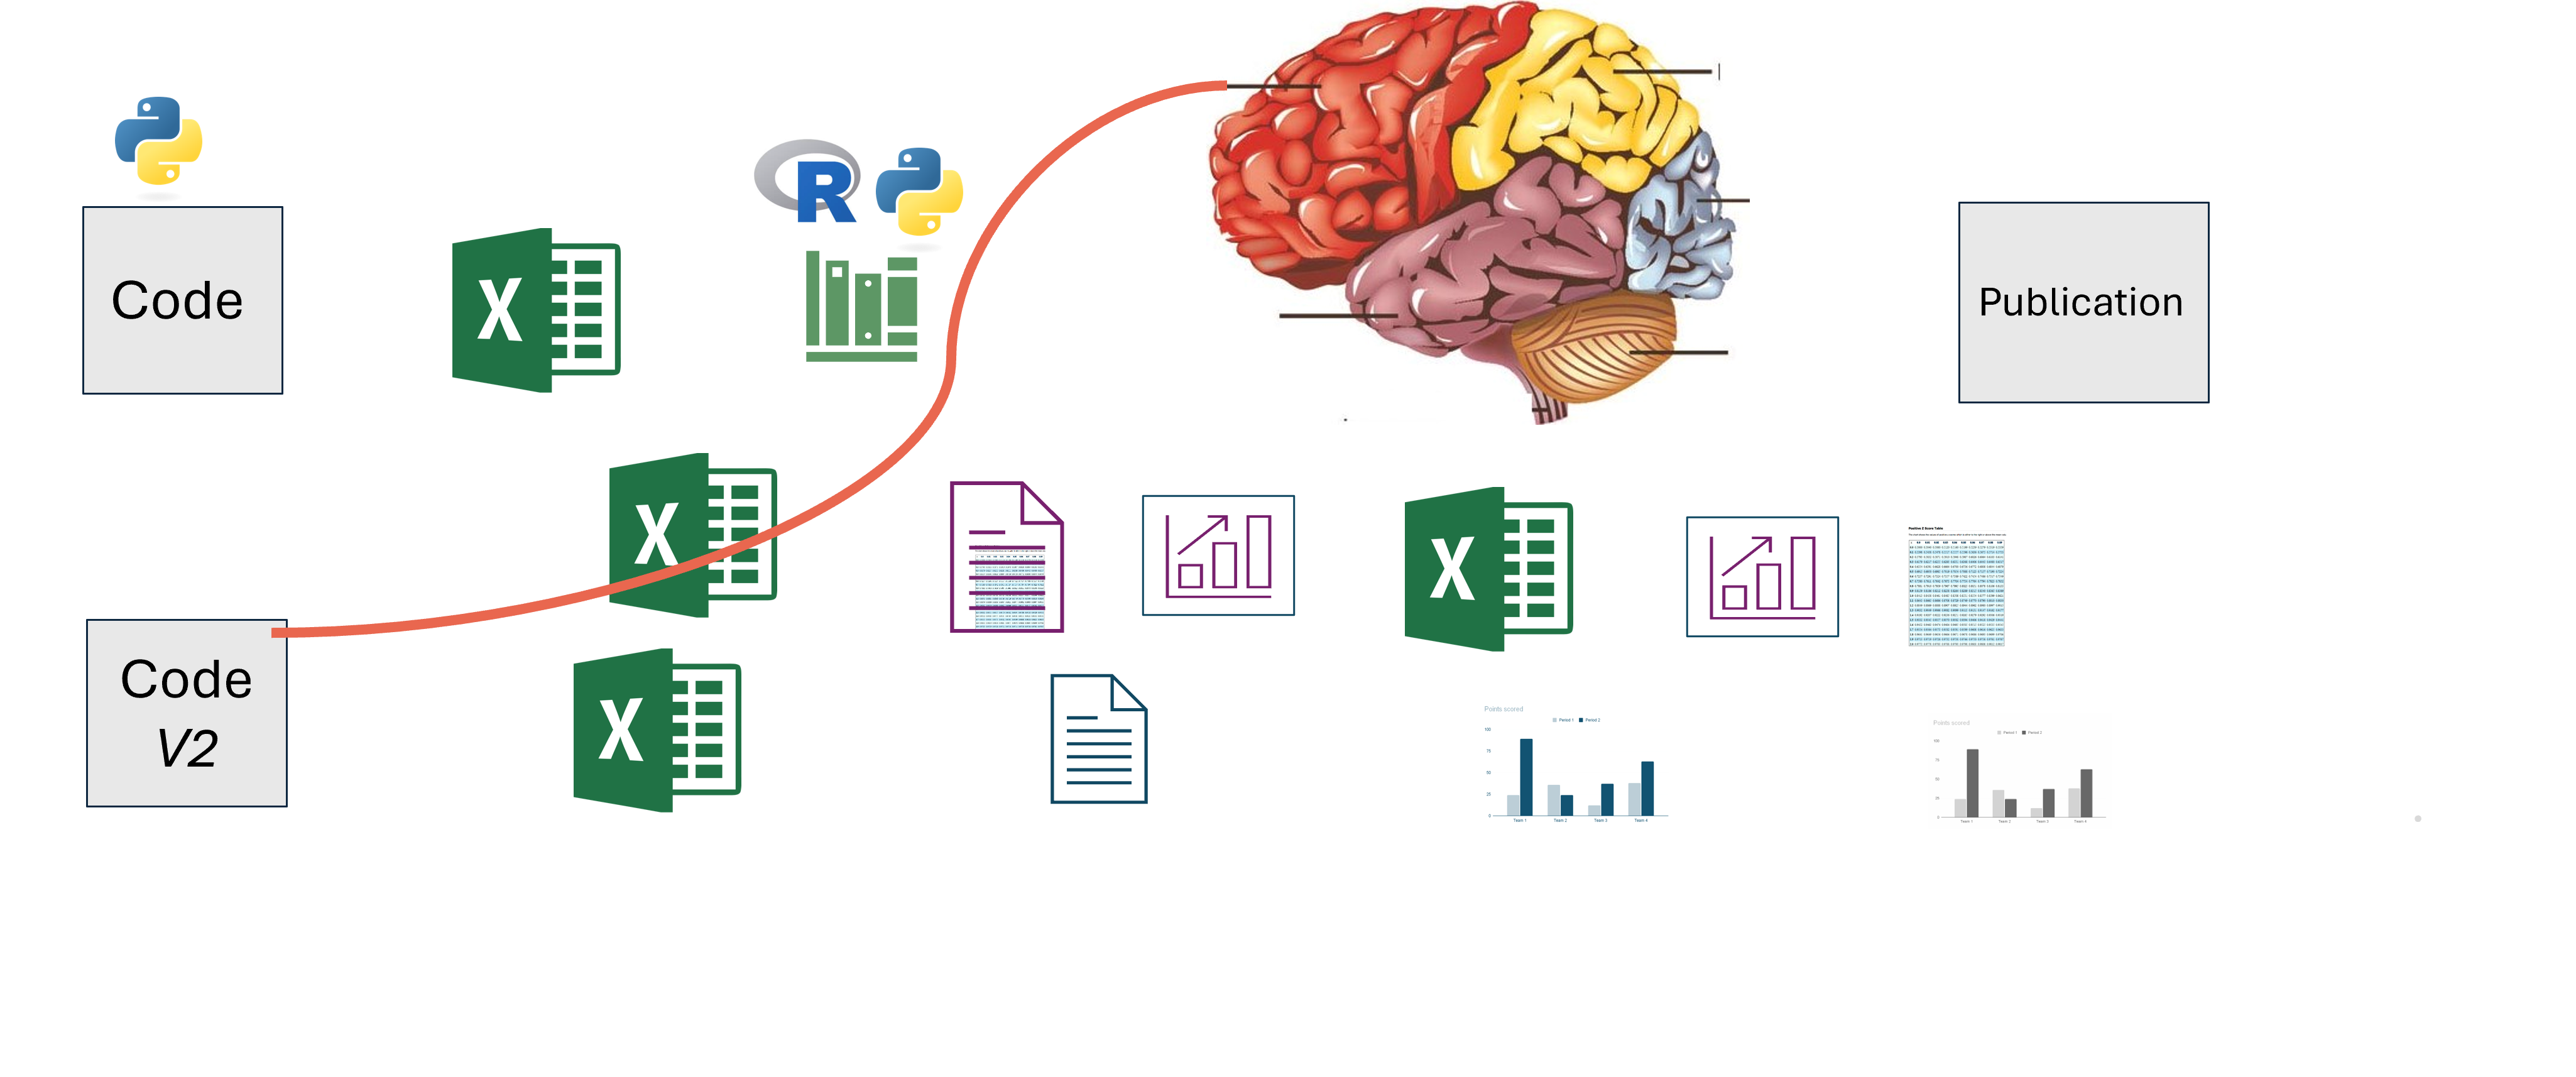
\includegraphics[width=1.0\textwidth]{Process16.png} }
        \only<5>{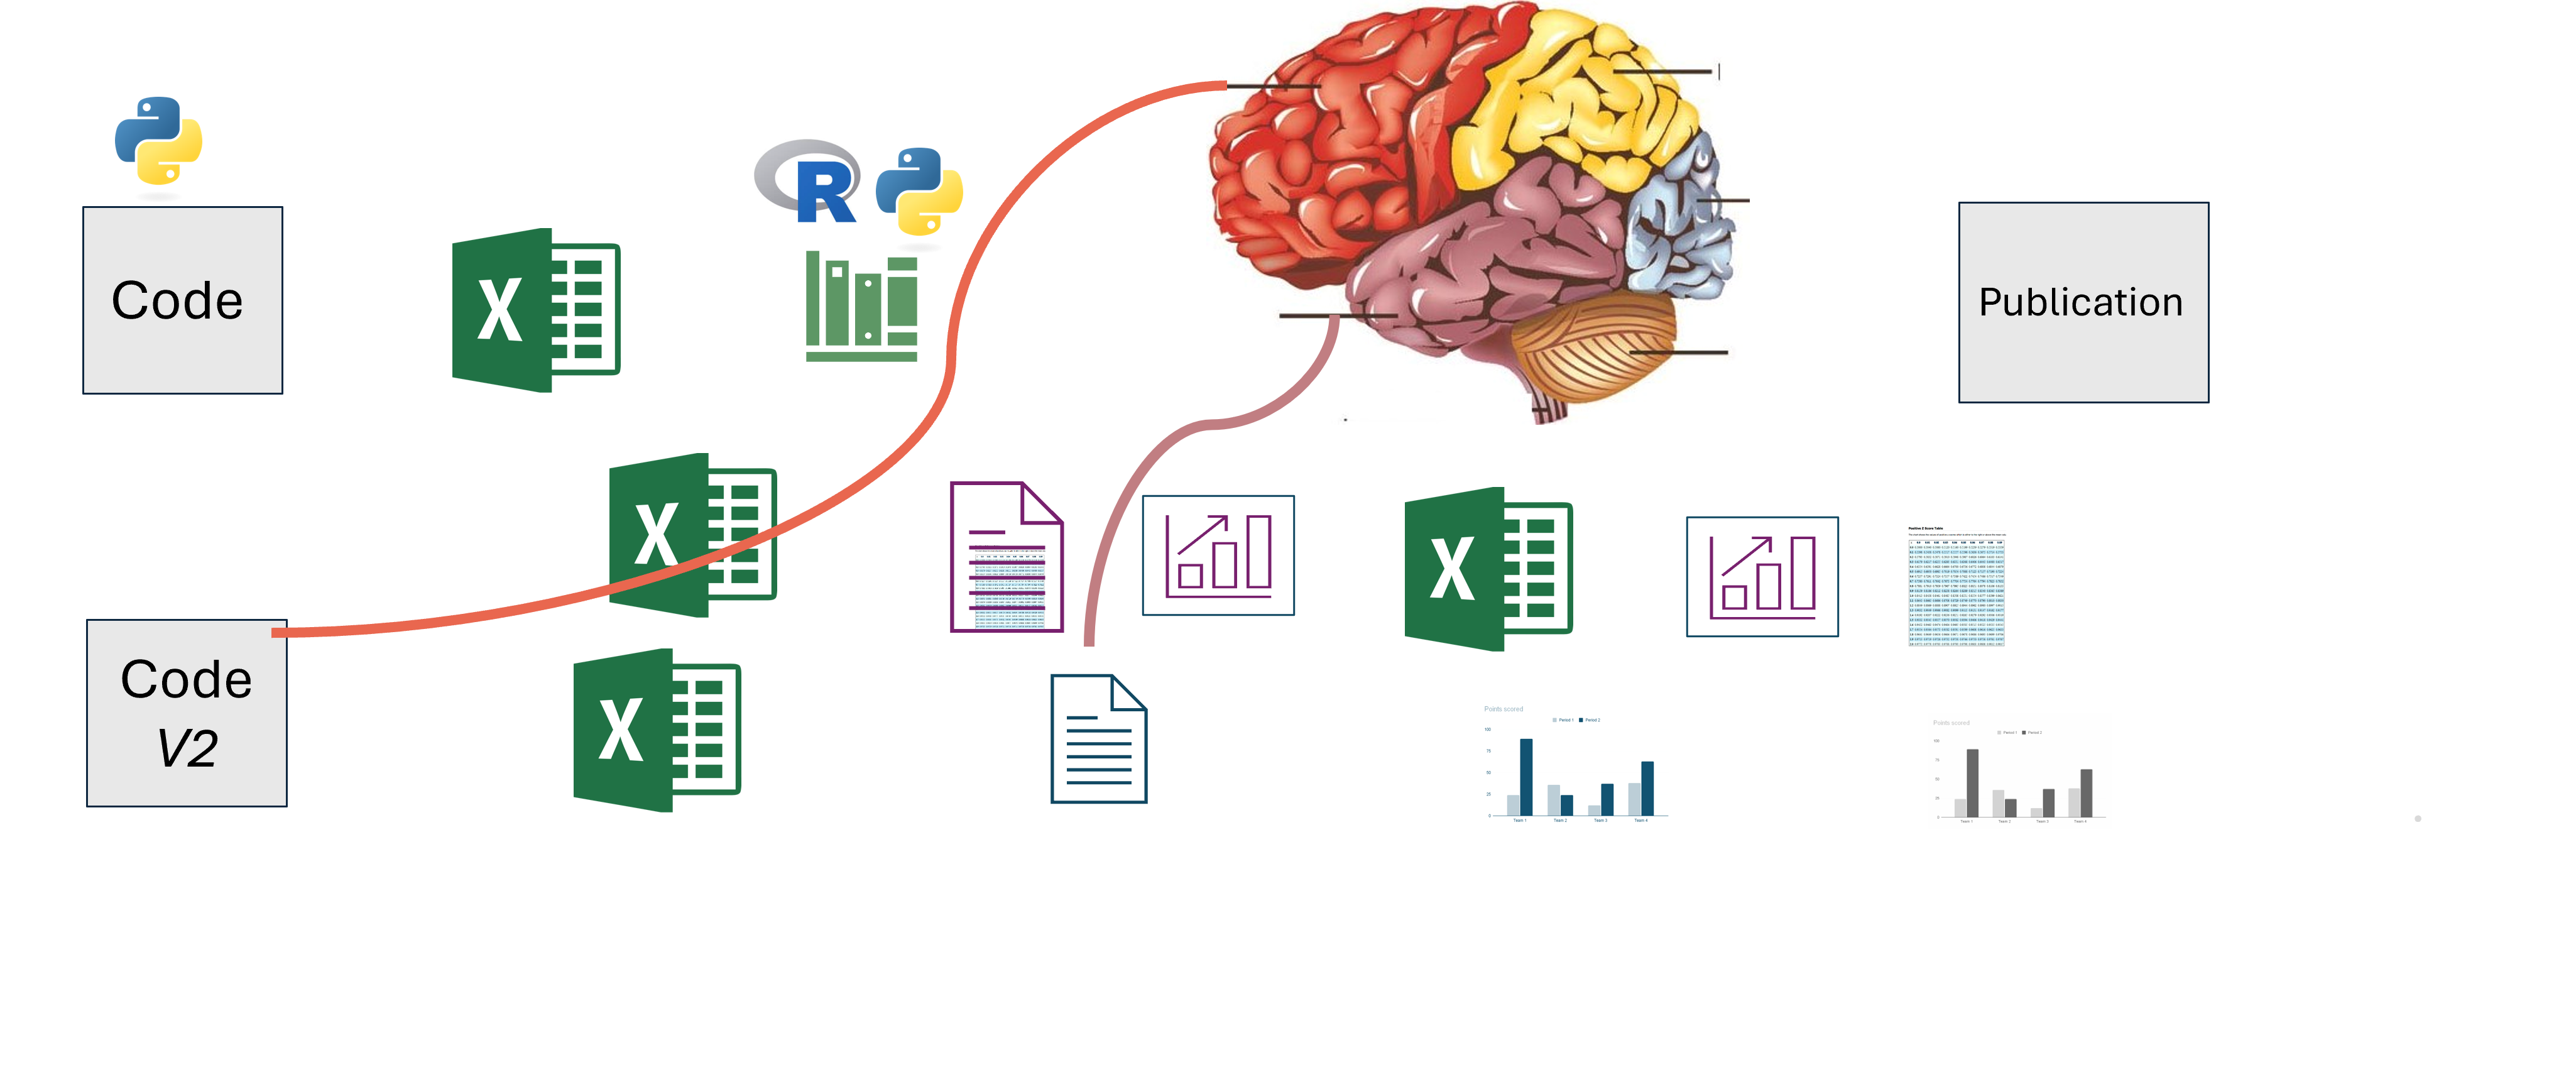
\includegraphics[width=1.0\textwidth]{Process17.png}}
        \only<6>{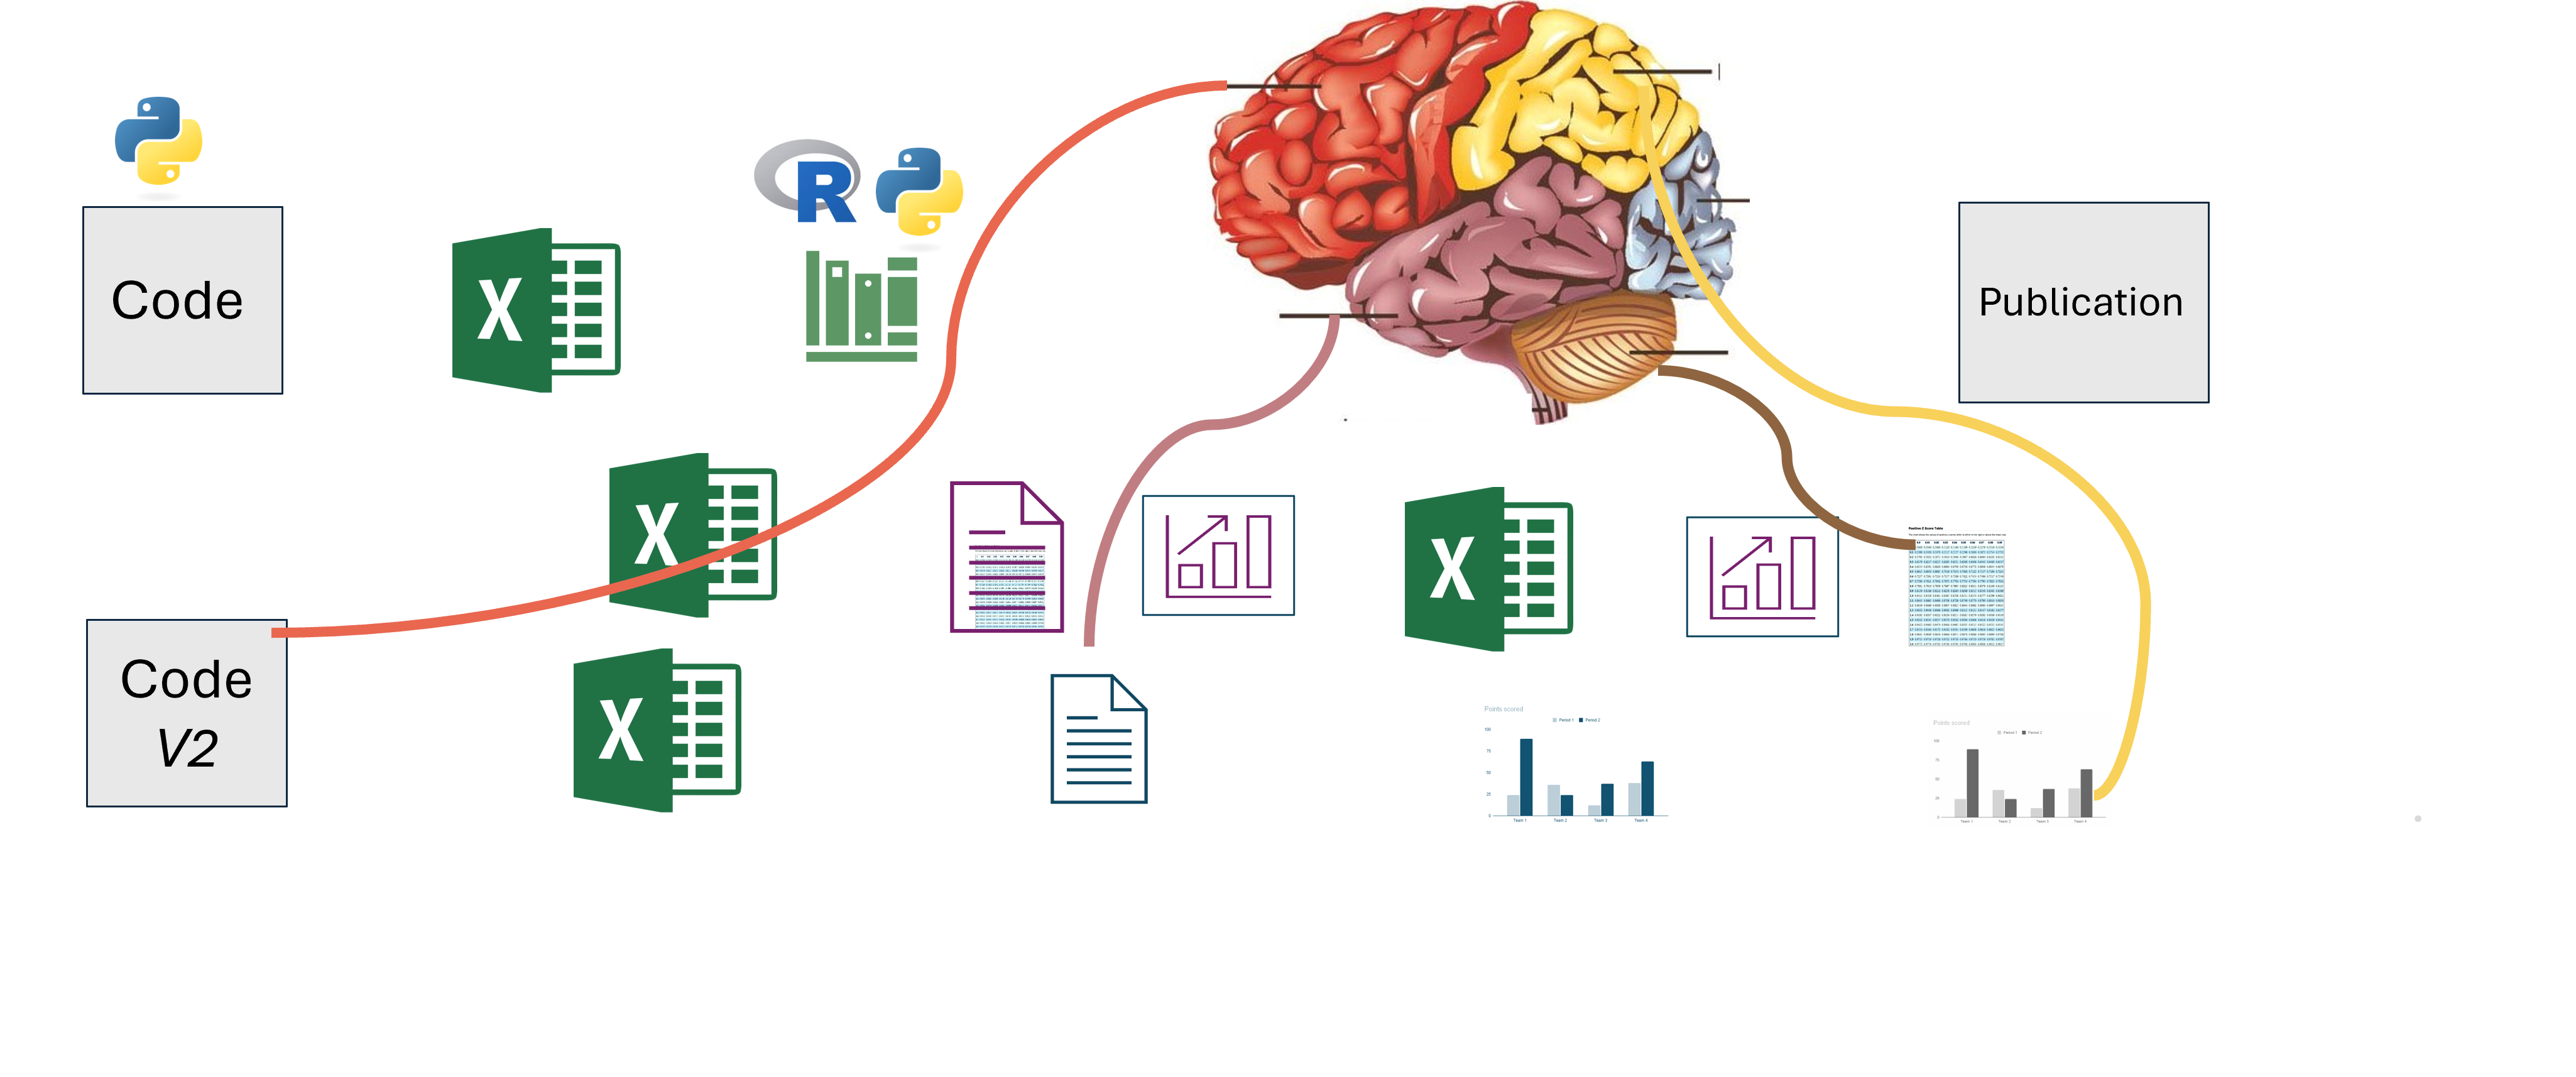
\includegraphics[width=1.0\textwidth]{Process18.png}}
        \only<7>{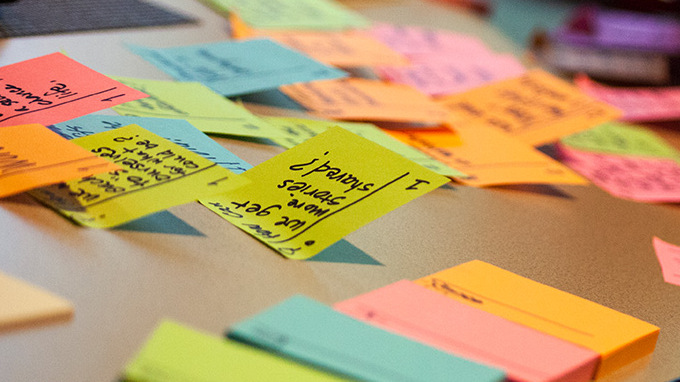
\includegraphics[width=1.0\textwidth]{Post-it.jpg} }
    \end{itemize}
    \end{column}
  \end{columns}
\end{frame}

\section{Issues}

\begin{frame}{What are the issues?}
  \begin{columns}[T]
    \begin{column}{0.5\textwidth}
      \begin{itemize}[<+->]
        \item Errors due to cut and paste
        \item Errors are difficult to track
        \item Each operator has his/her own approach
        \item Several versions of code may coexist
        \item The steps aren't recorded
        \item Reproducibility is not granted
       % \item Quality control is hard
      \end{itemize}
    \end{column}
    \begin{column}{0.5\textwidth}
    \begin{itemize}
        \item[]  \only<1-2>{\href{https://www.bbc.com/news/technology-54423988}{ 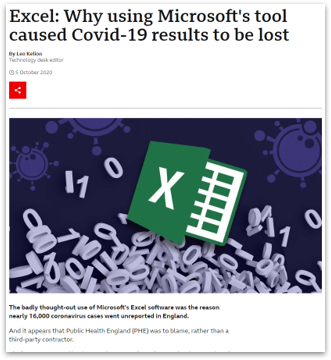
\includegraphics[width=1.0\textwidth]{ExcelUK.png}}}
         \only<3>{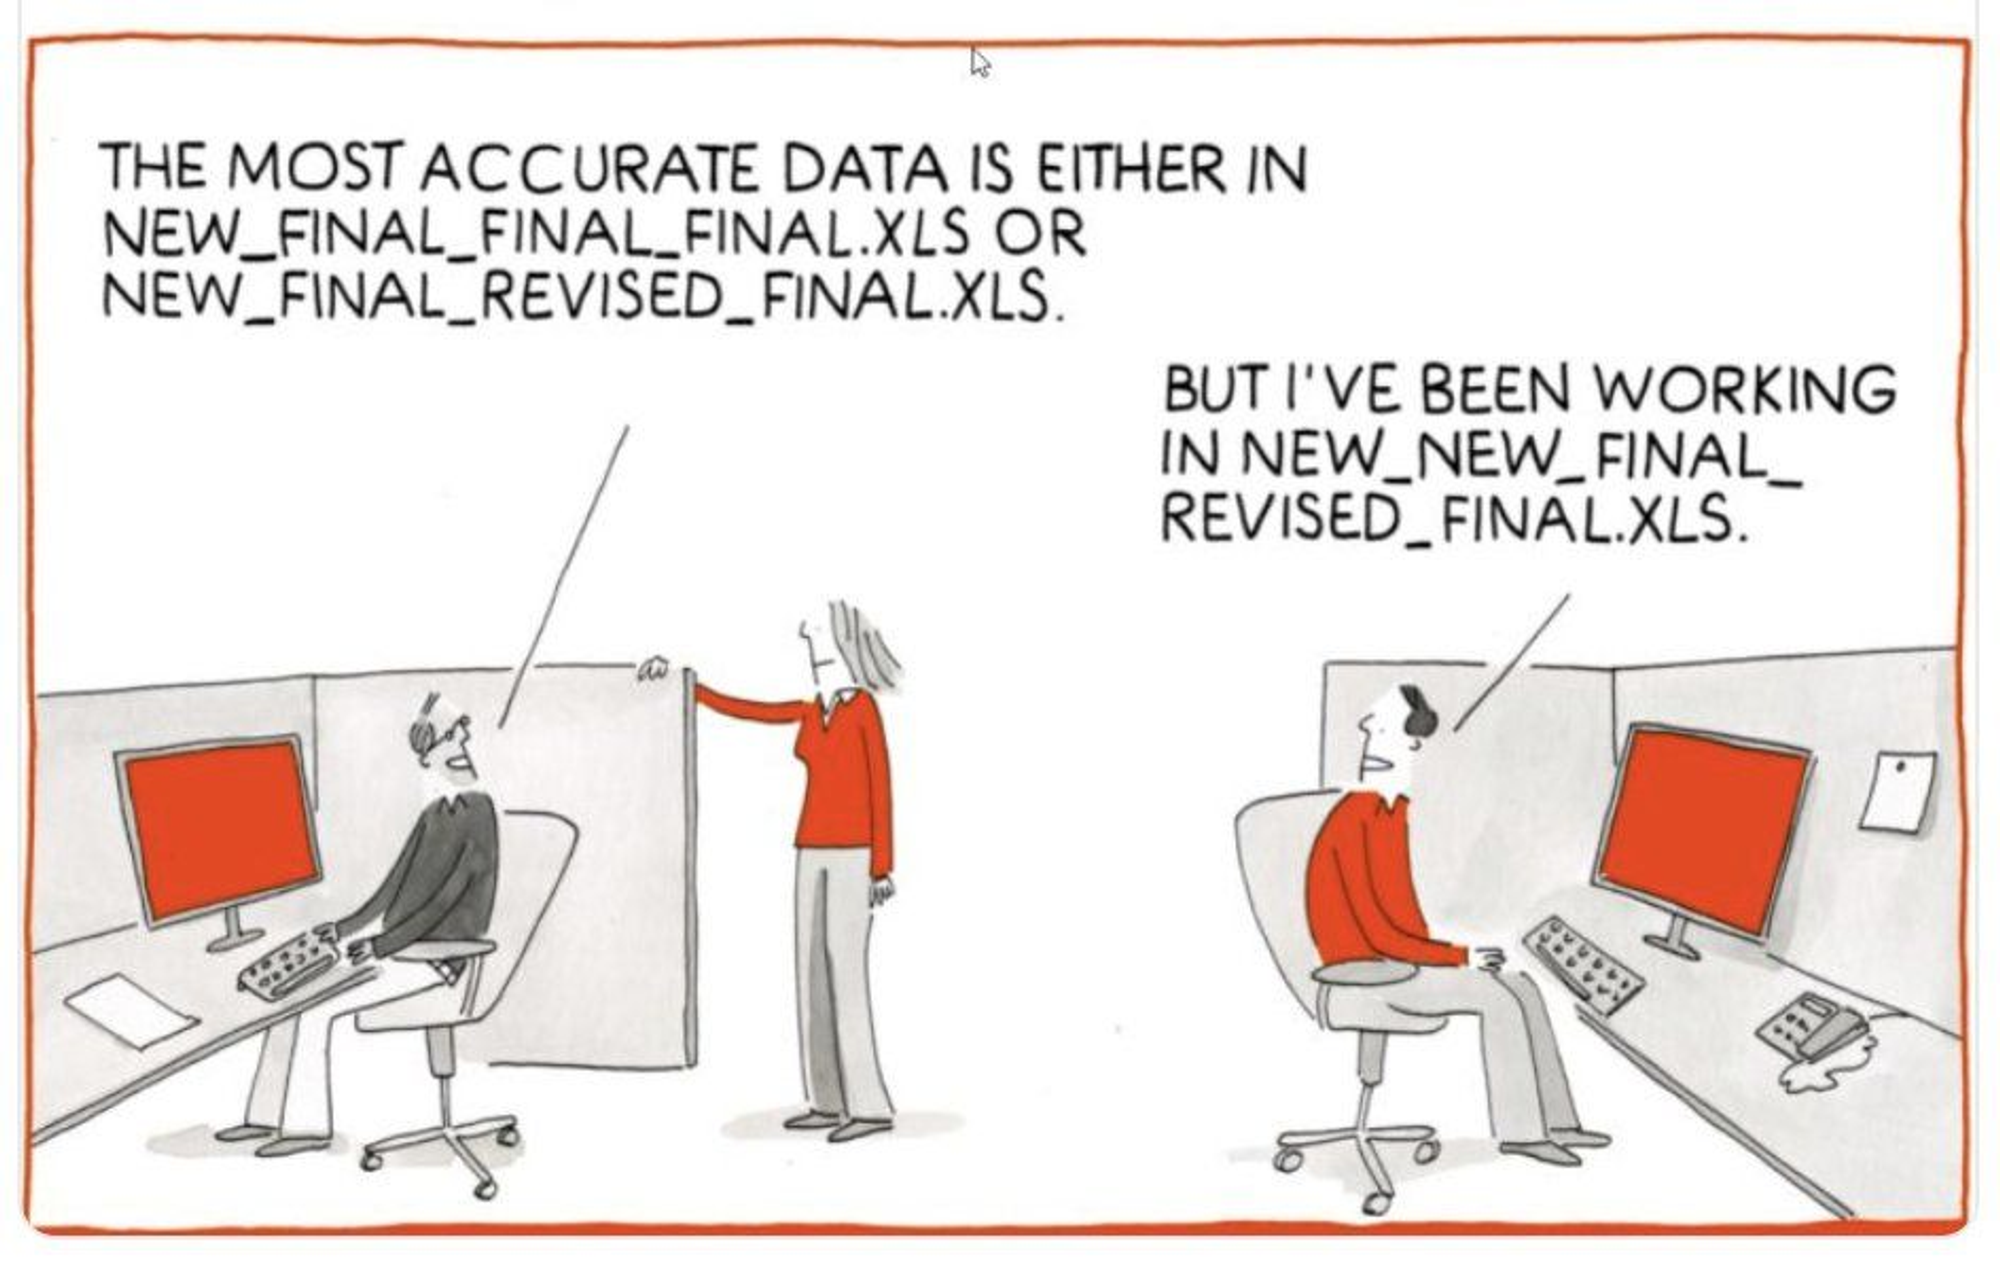
\includegraphics[width=1.0\textwidth]{FinalFinalVersion.png}}
         \only<4-5>{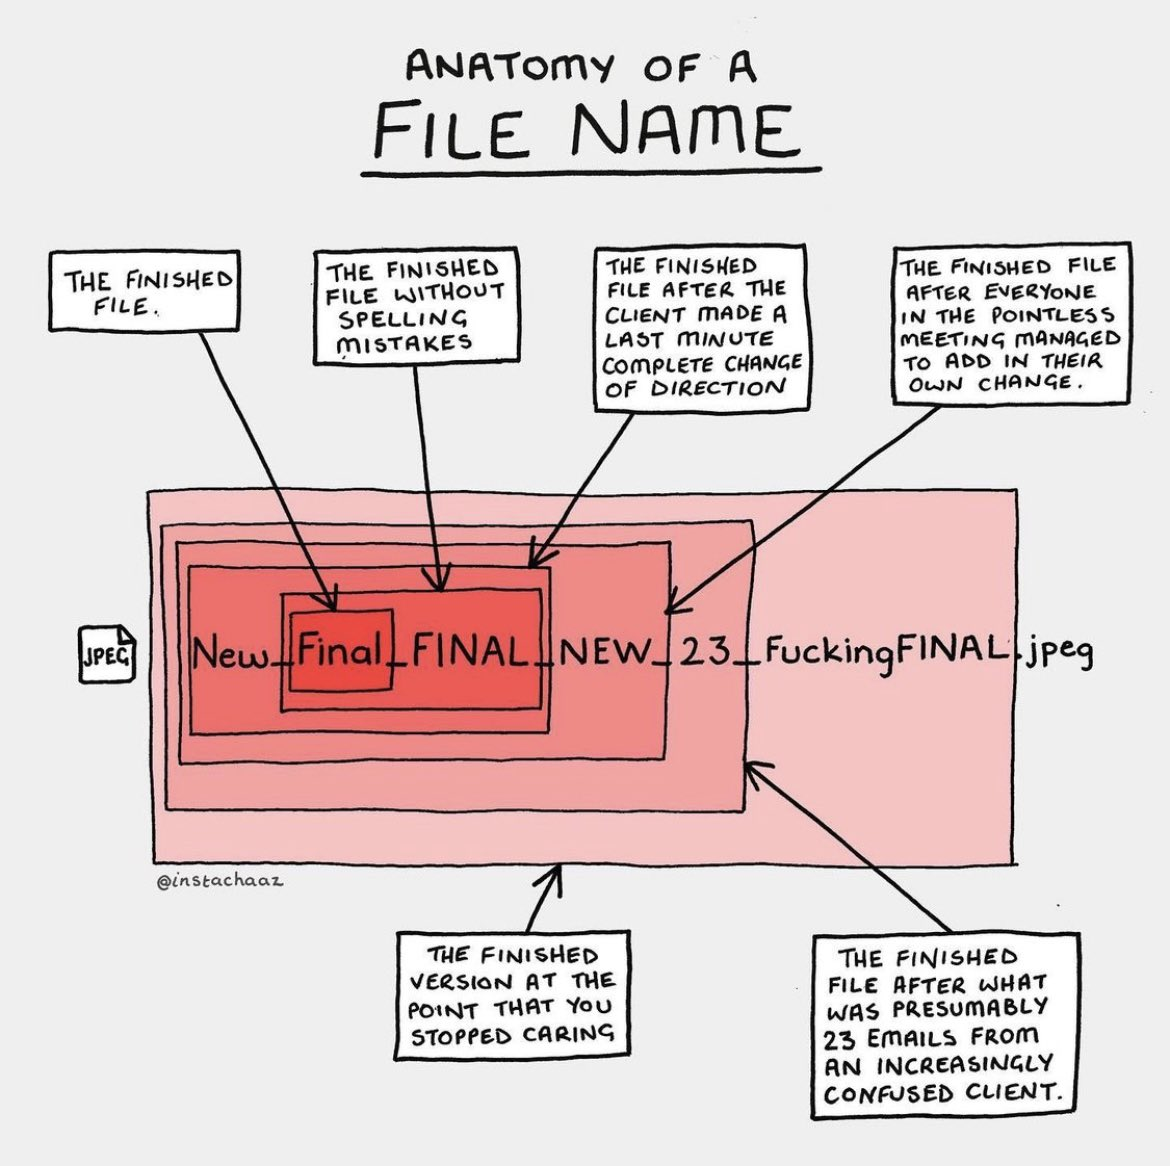
\includegraphics[width=1.0\textwidth]{AnatomyOfaFile.png}}
         \only<6>{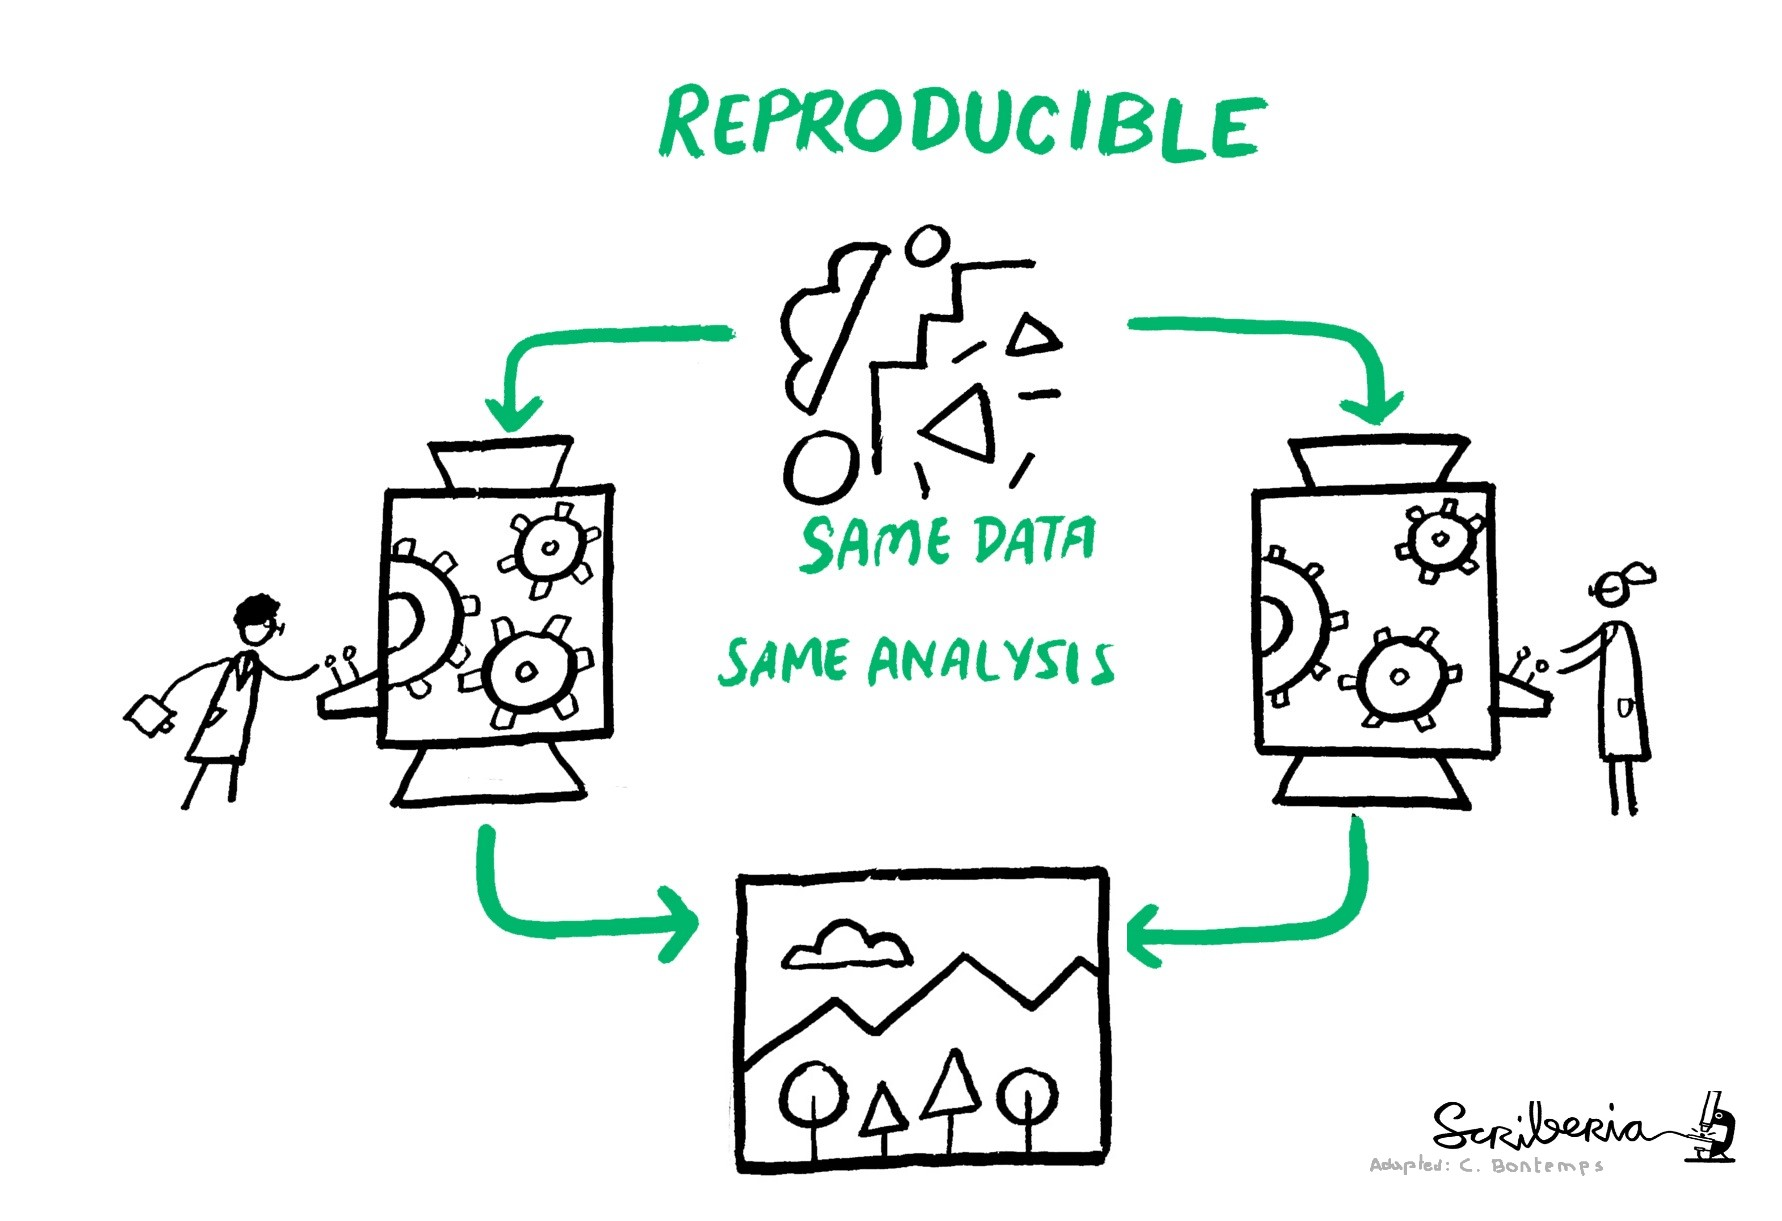
\includegraphics[width=1.0\textwidth]{Reproducible.jpg}}
         \end{itemize}
    \end{column}
  \end{columns}
\end{frame}

% Other slides should go here...

\section{RAP}  % Better practices

\begin{frame}{What is A Reproducible Analytical Pipeline?}
  \begin{columns}[T]
    \begin{column}{0.5\textwidth}
      \begin{itemize}[<+->]
        \item It is a process % or a way to think a process
        \item It is automated
        \item It is easily reproducible
        \item It minimises mistakes
        \item It is fast
        \item It builds trust
      \end{itemize}
    \end{column}
    \begin{column}{0.5\textwidth}
    \begin{itemize}
        \item[] 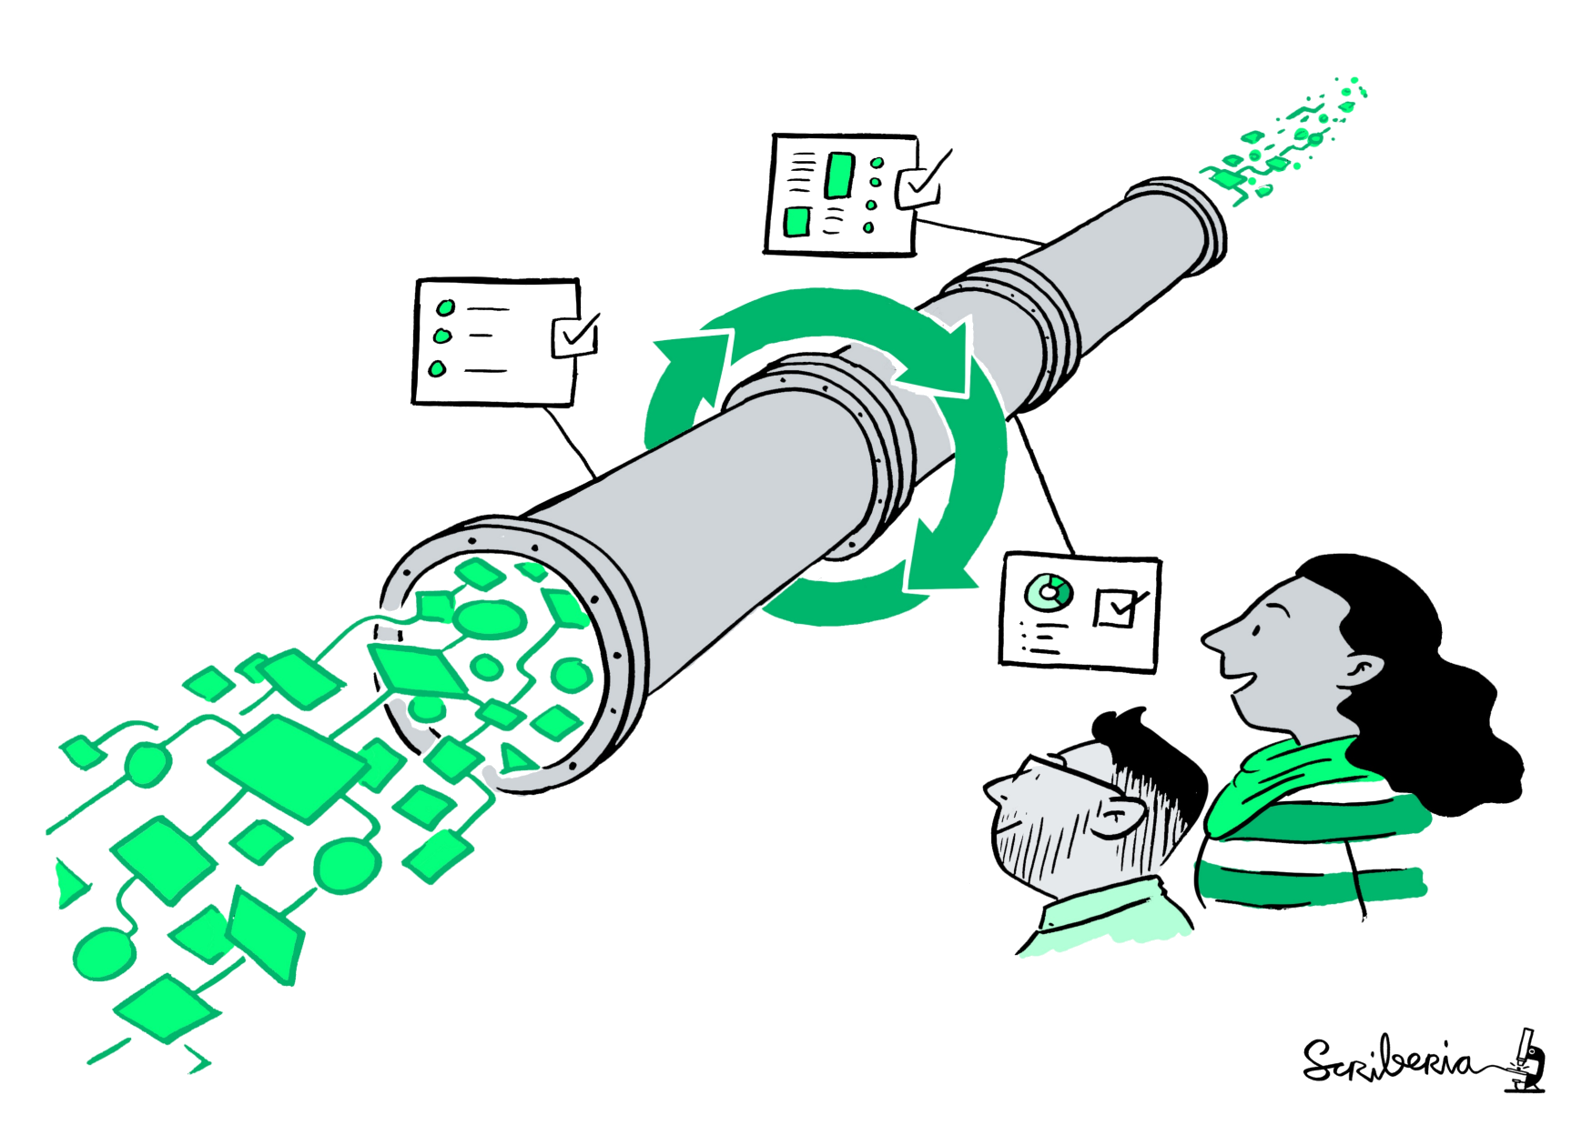
\includegraphics[width=1.0\textwidth]{ReusablePipeline.png}
    \end{itemize}
    \end{column}
  \end{columns}
\end{frame}

\begin{frame}{What does a RAP look like?}
 \begin{center}
  \begin{itemize}
        \only<1>{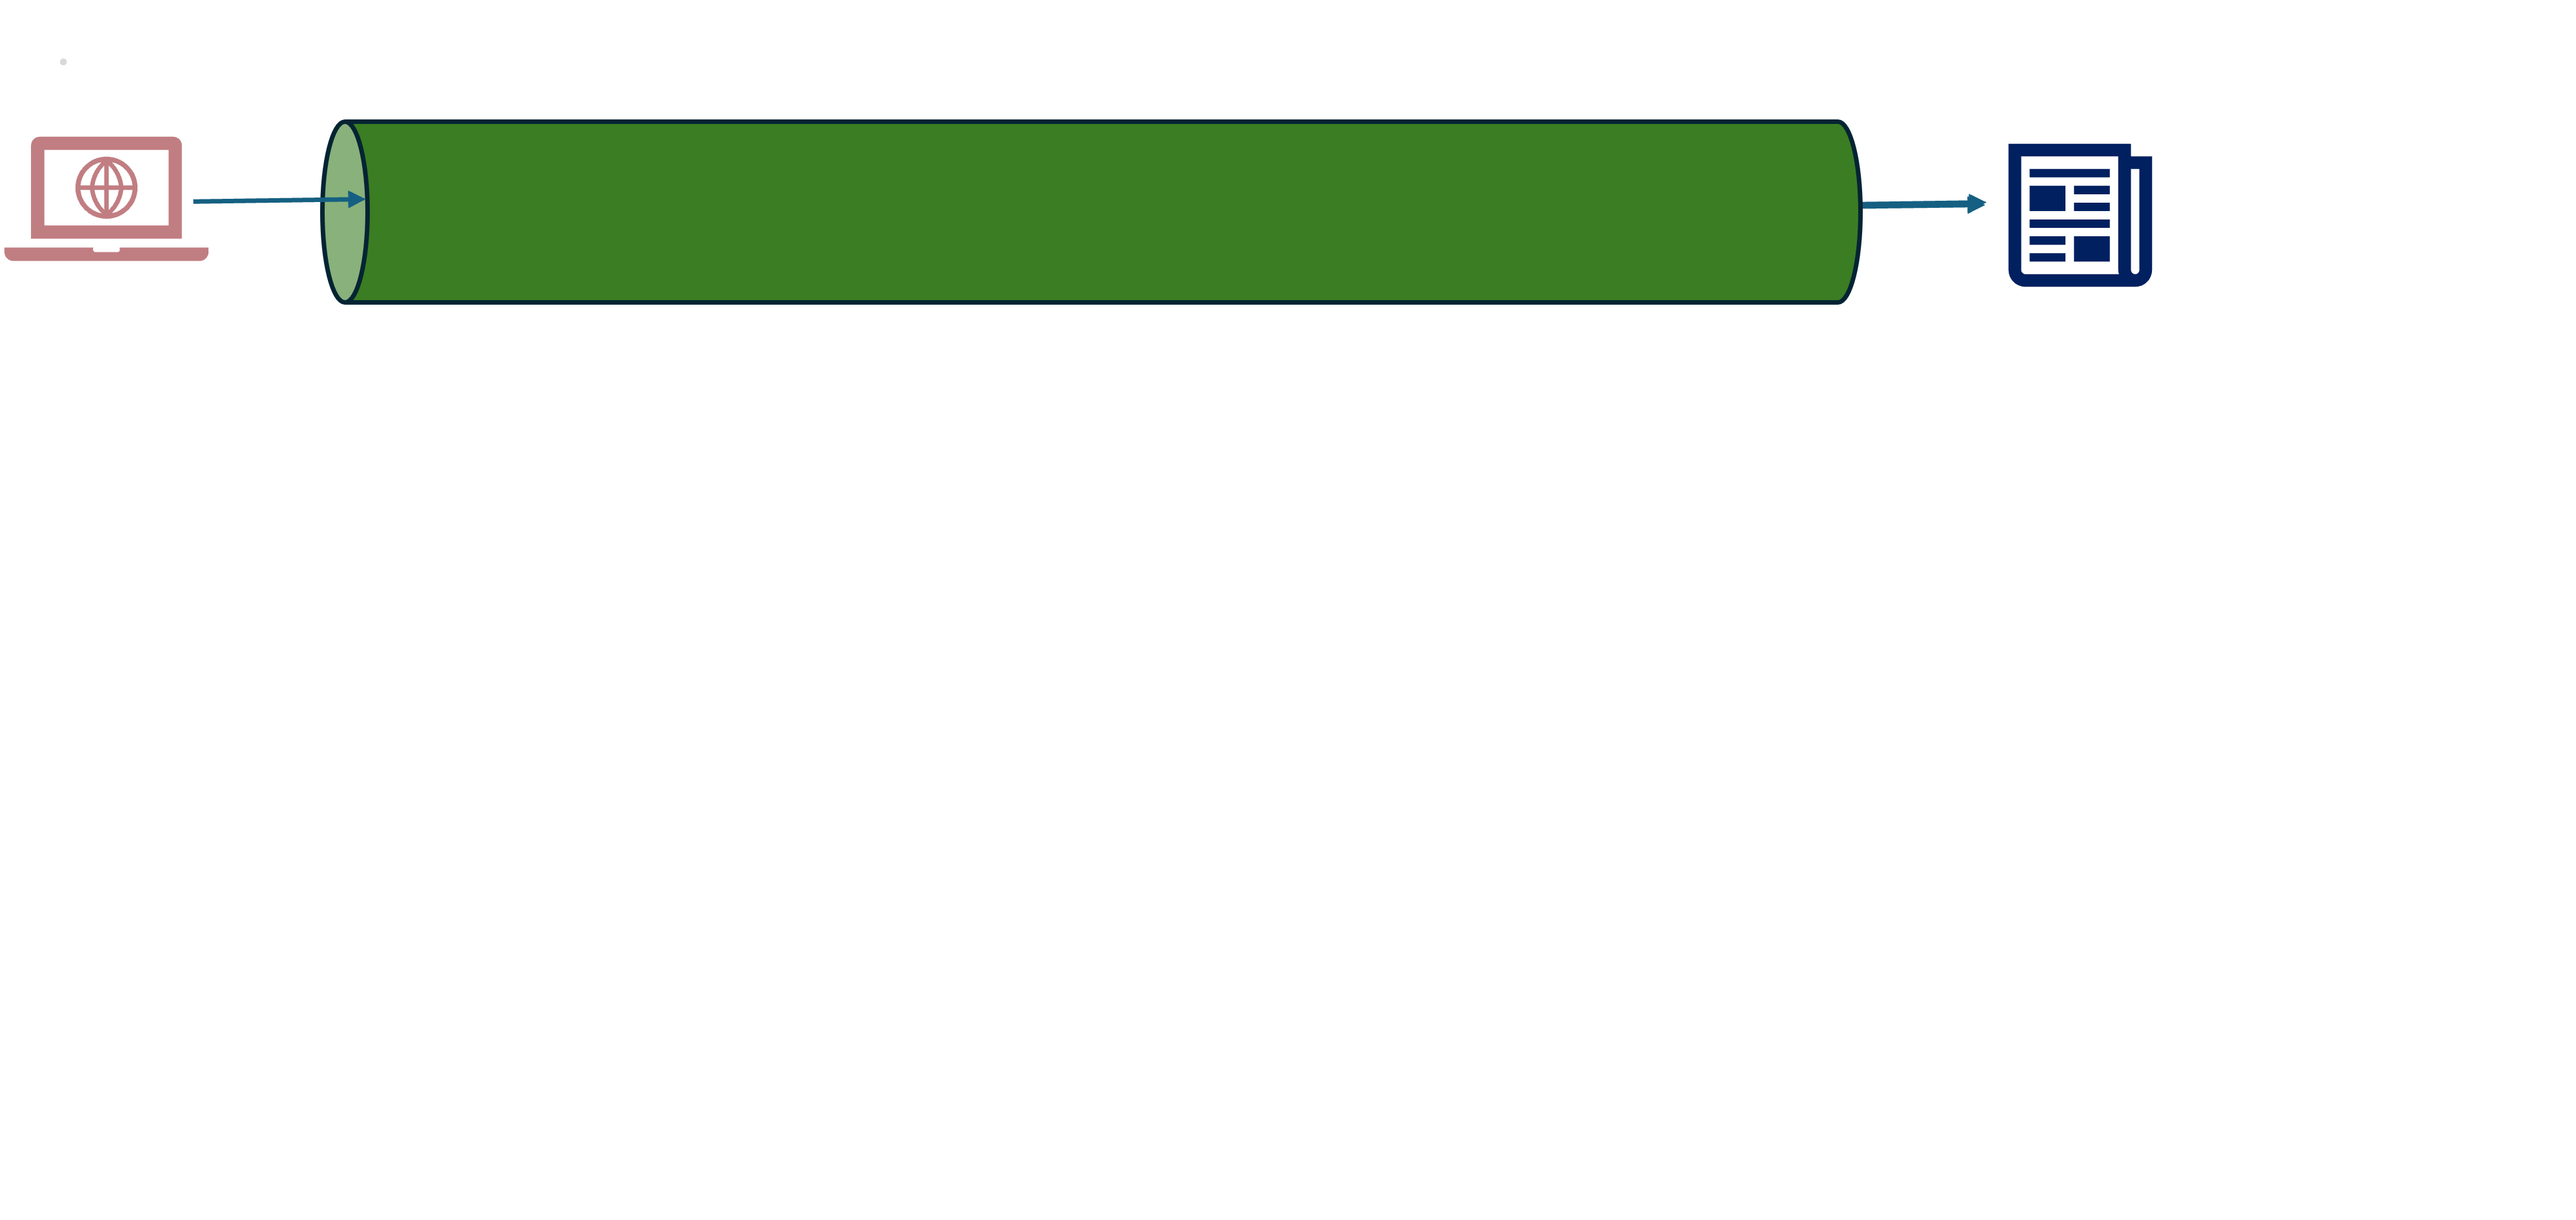
\includegraphics[width=0.8\textwidth]{Pipeline1.png} \\ Comment 1}
        \only<2>{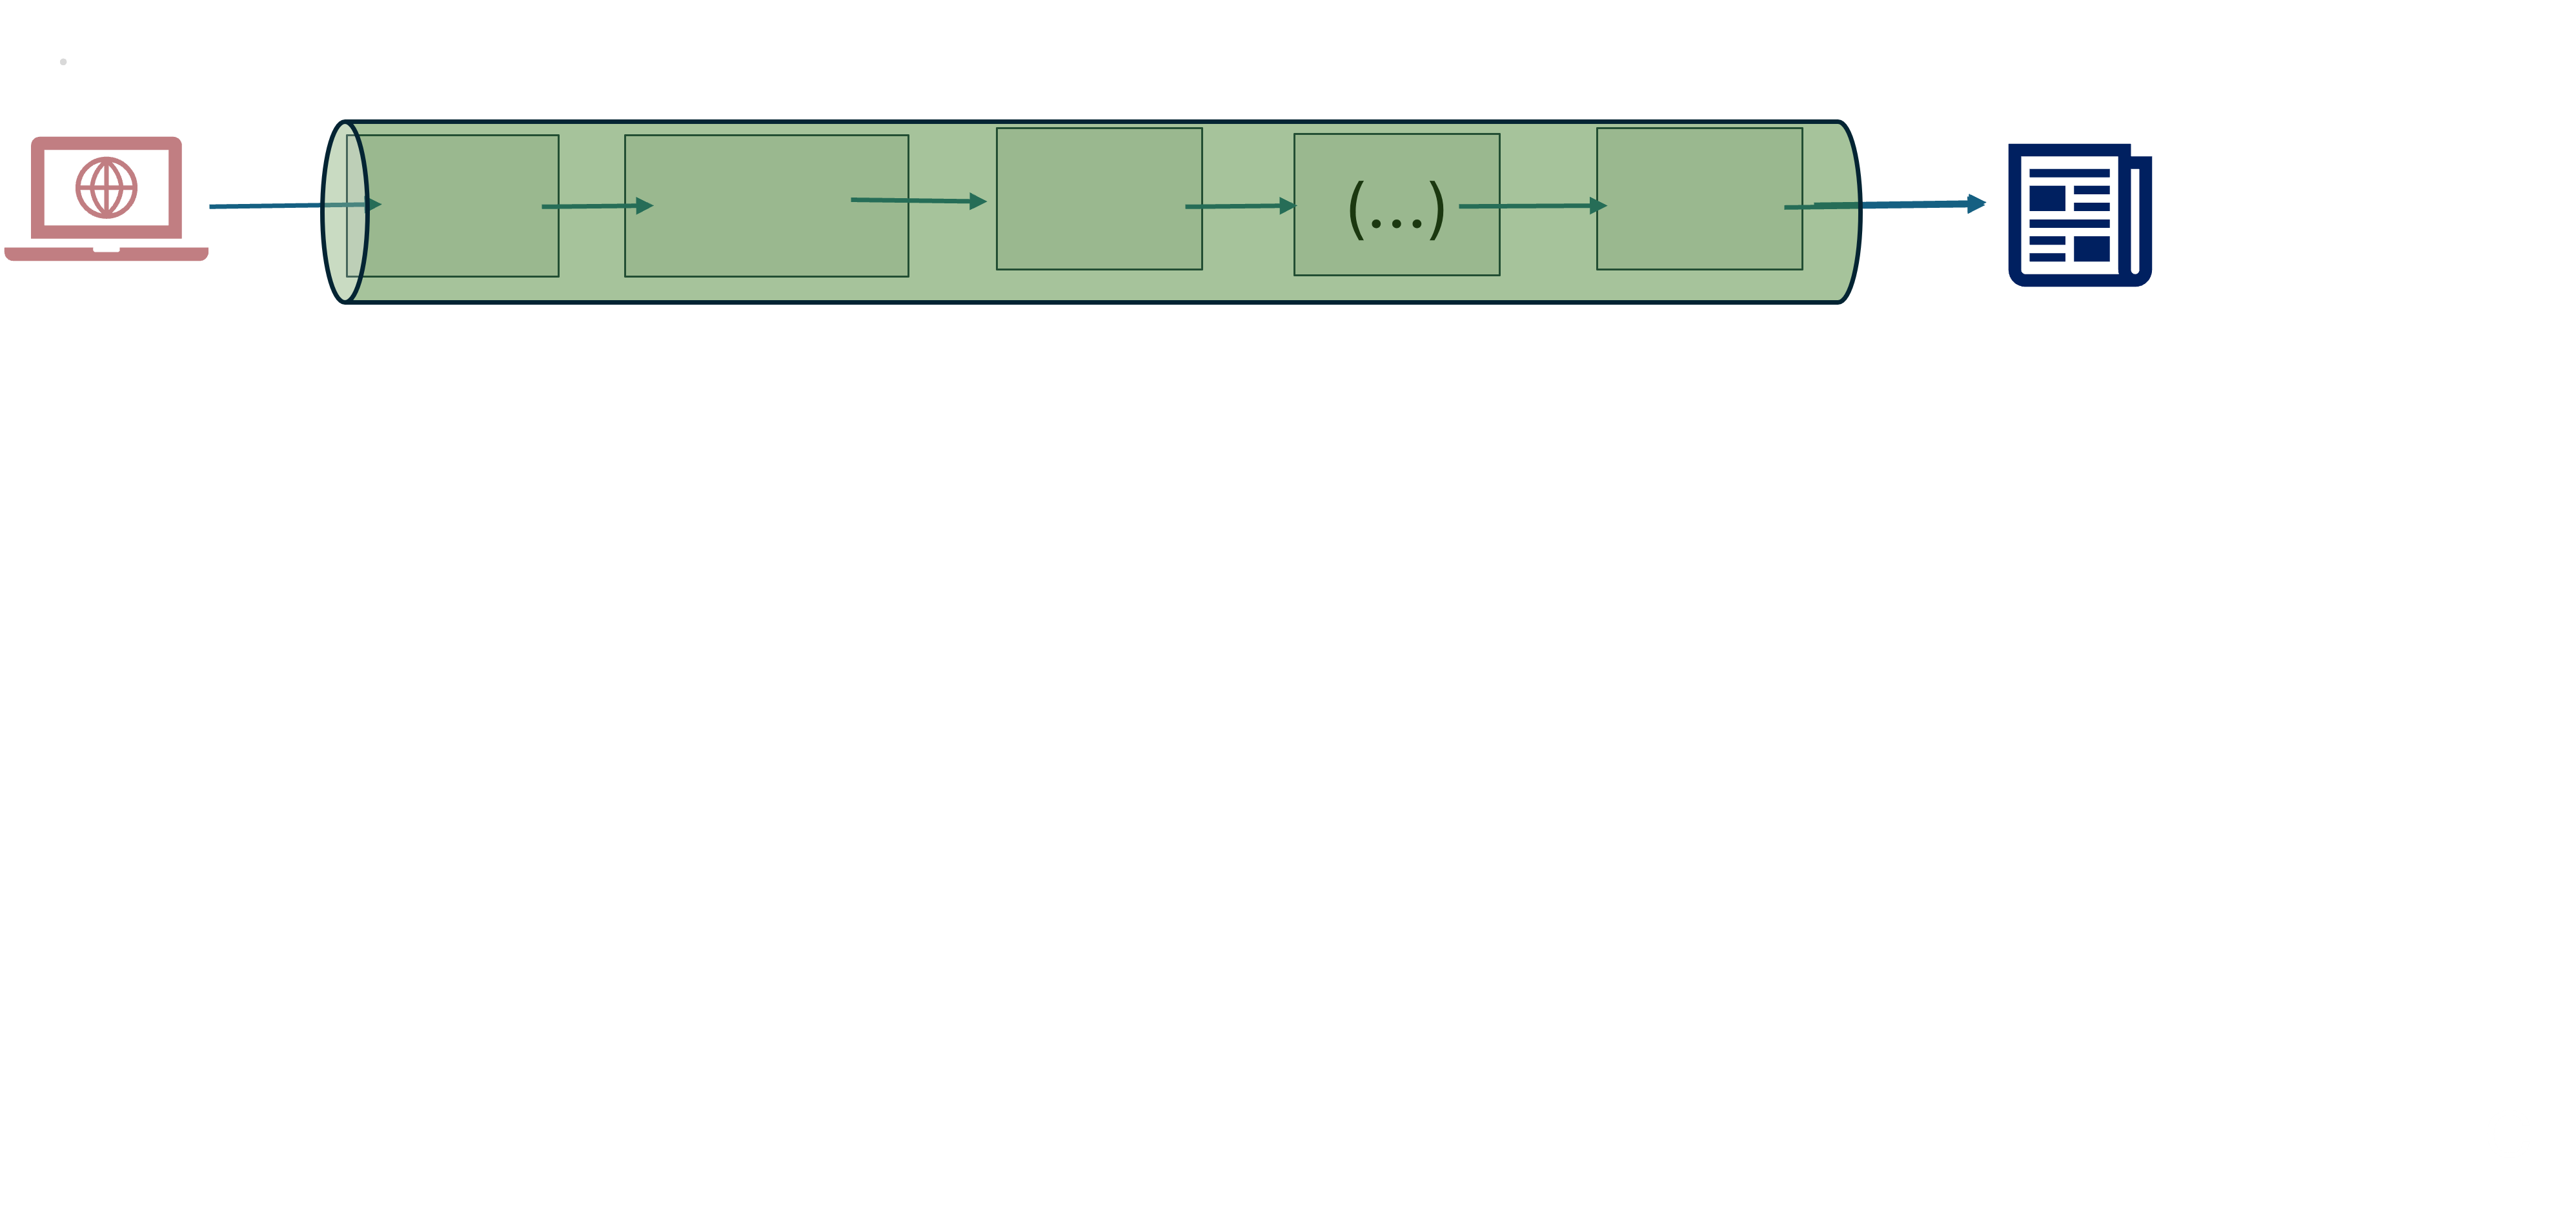
\includegraphics[width=0.8\textwidth]{Pipeline2.png} \\ Comment 2}
        \only<3>{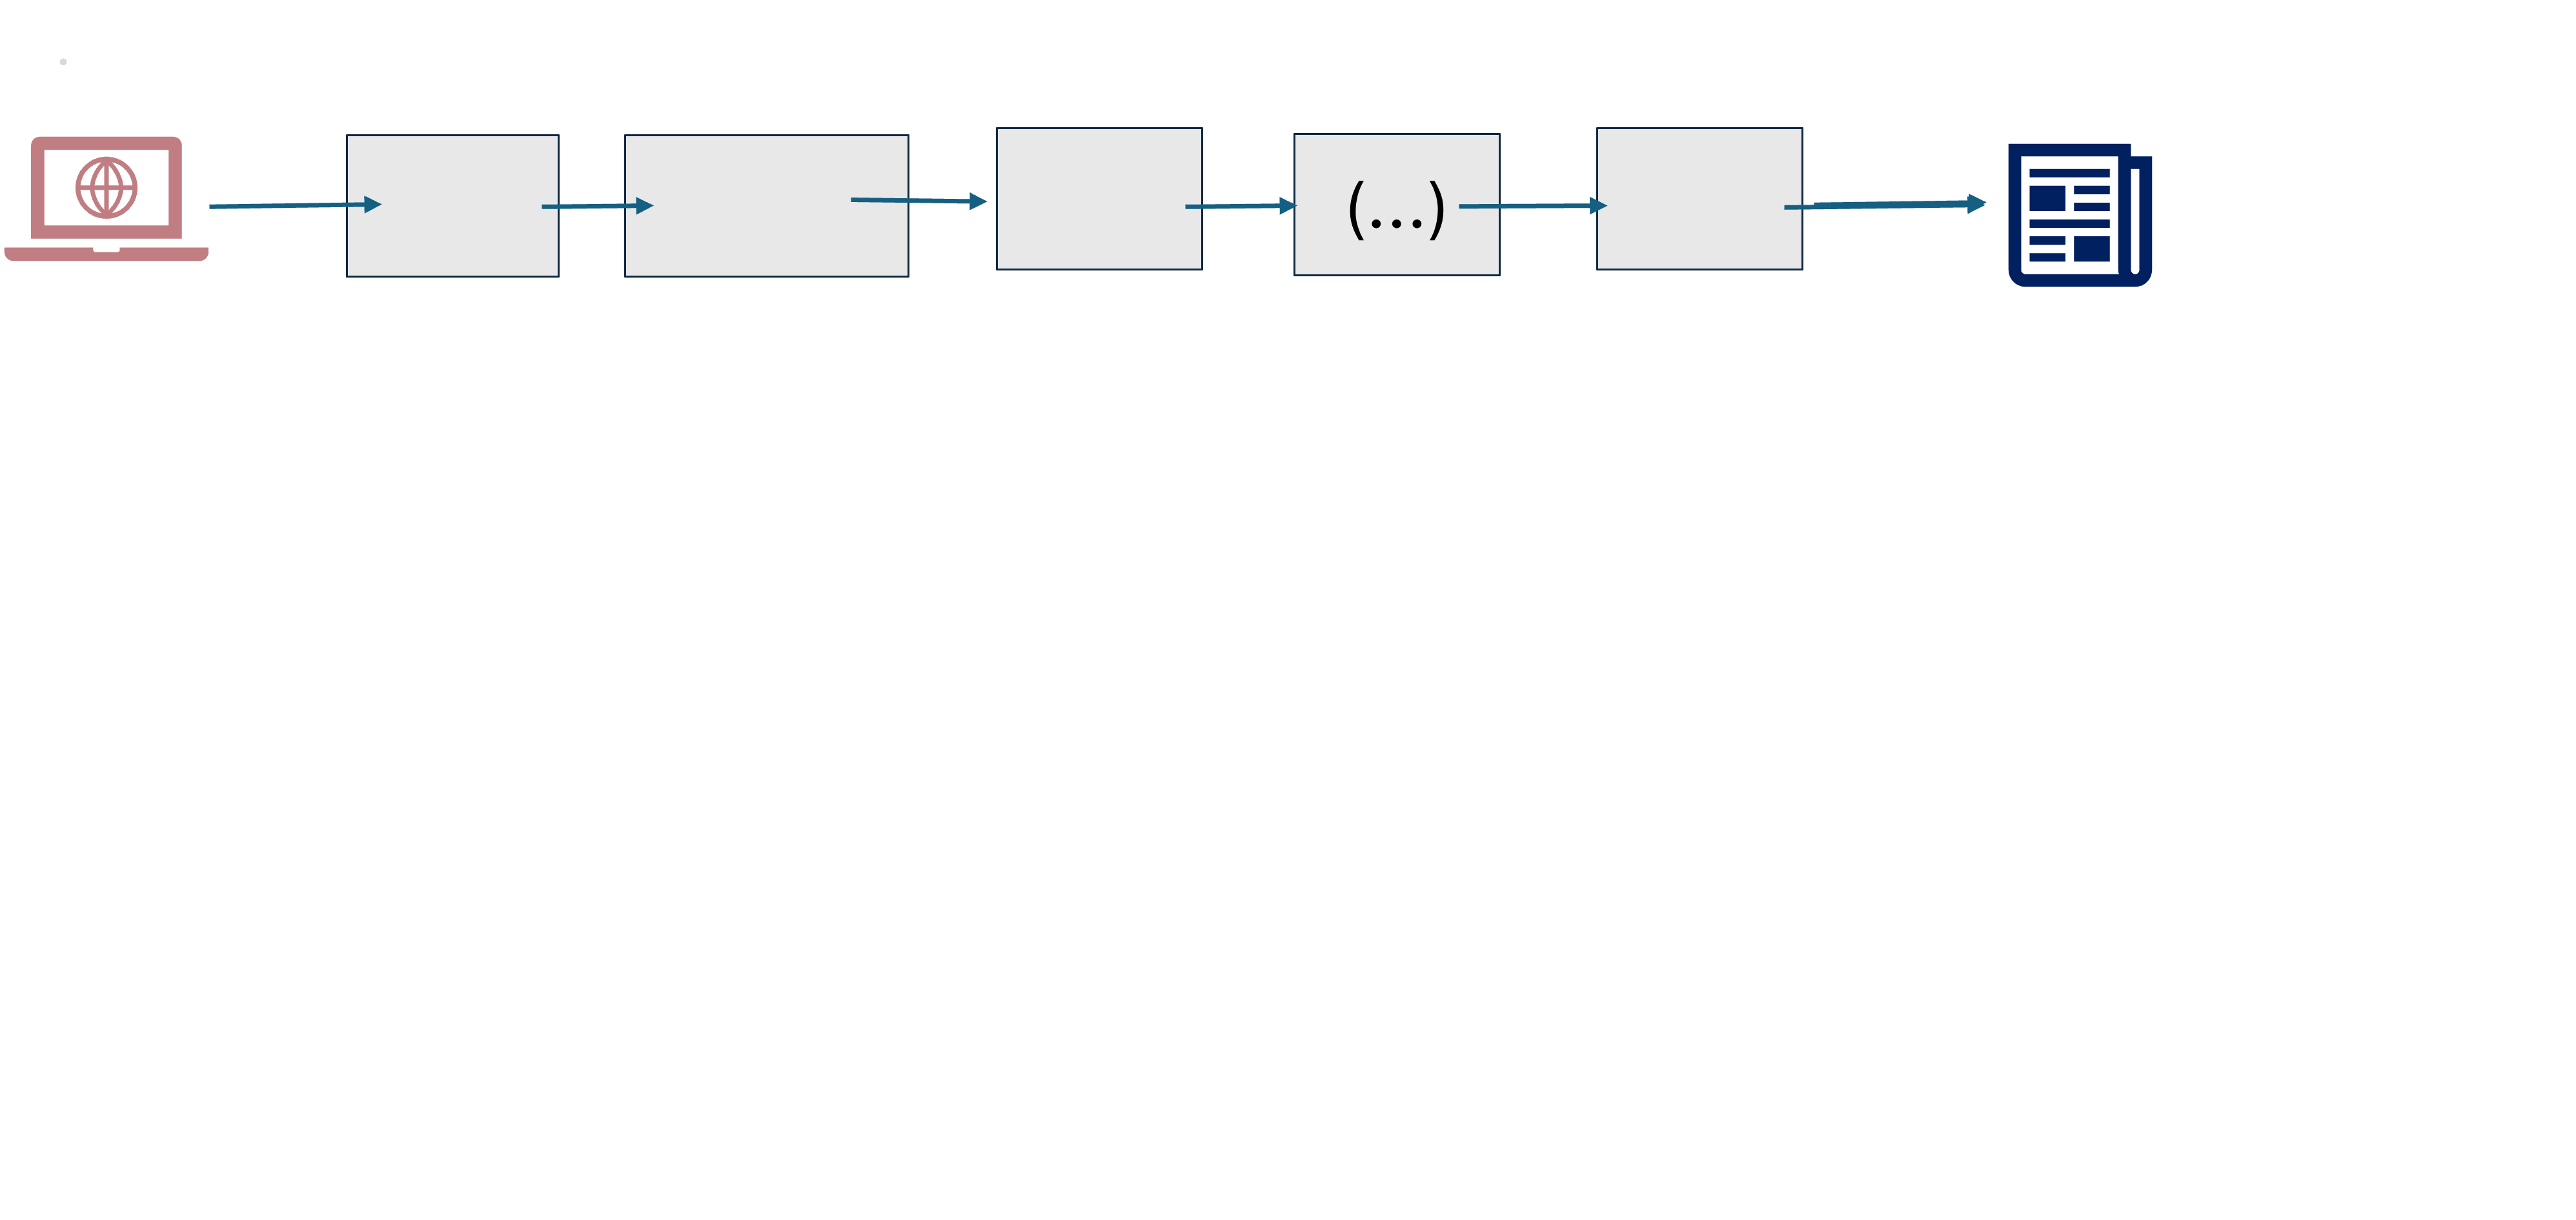
\includegraphics[width=0.8\textwidth]{Pipeline3.png} \\ Comment 3}
        \only<4>{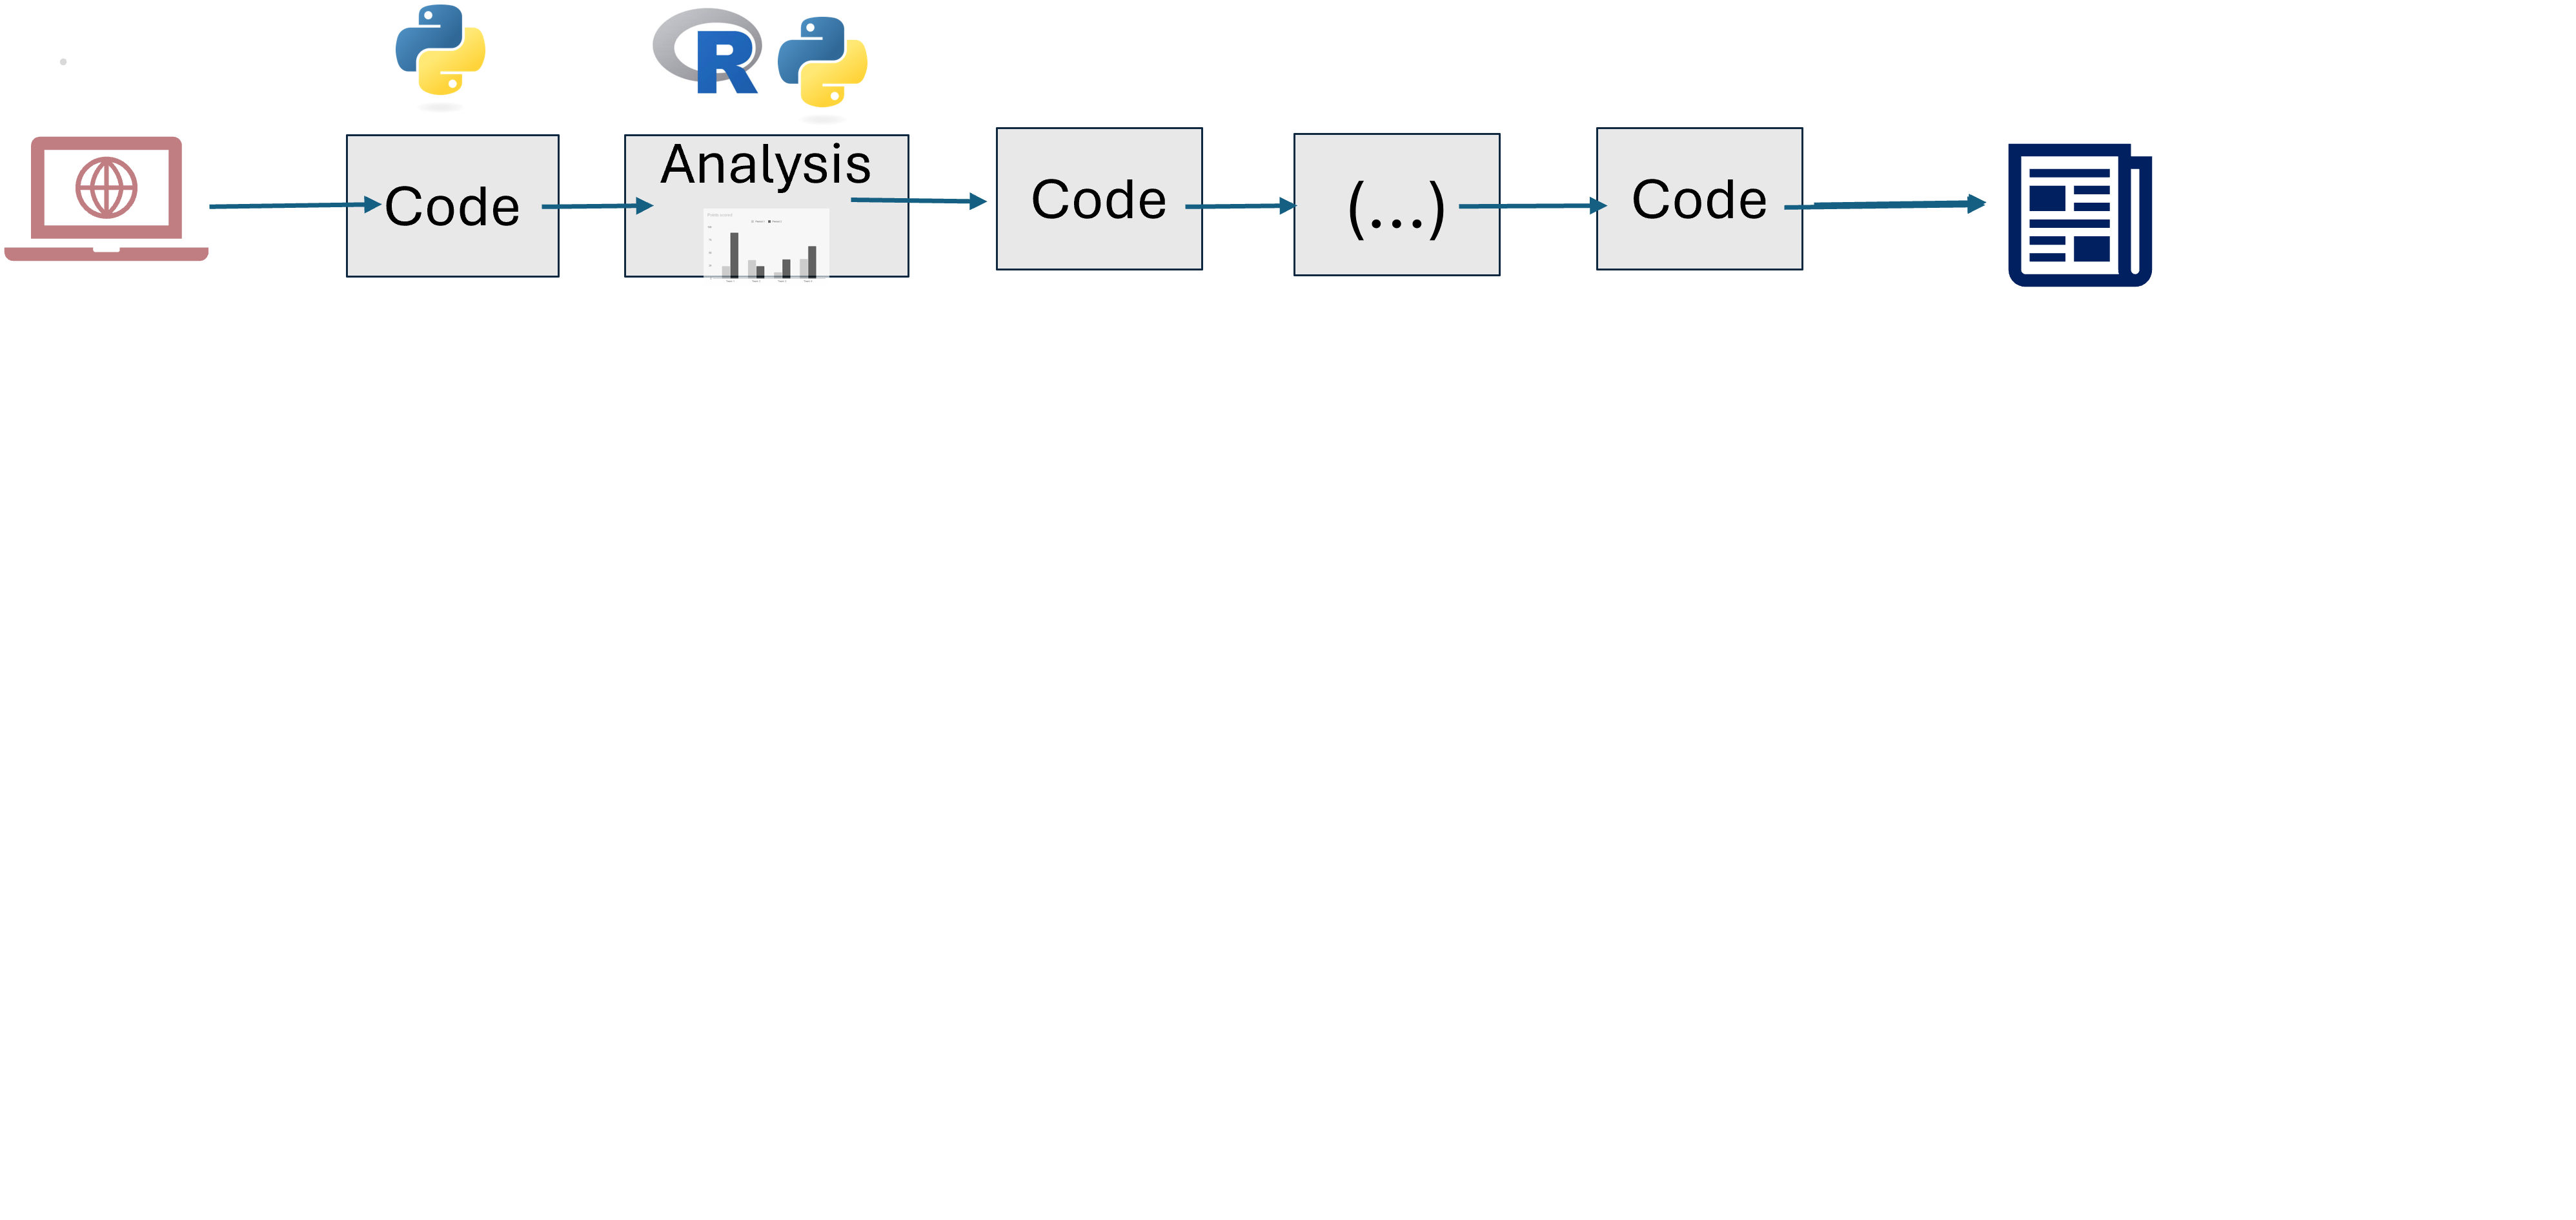
\includegraphics[width=0.8\textwidth]{Pipeline4.png} \\ Comment 4}
        \only<5>{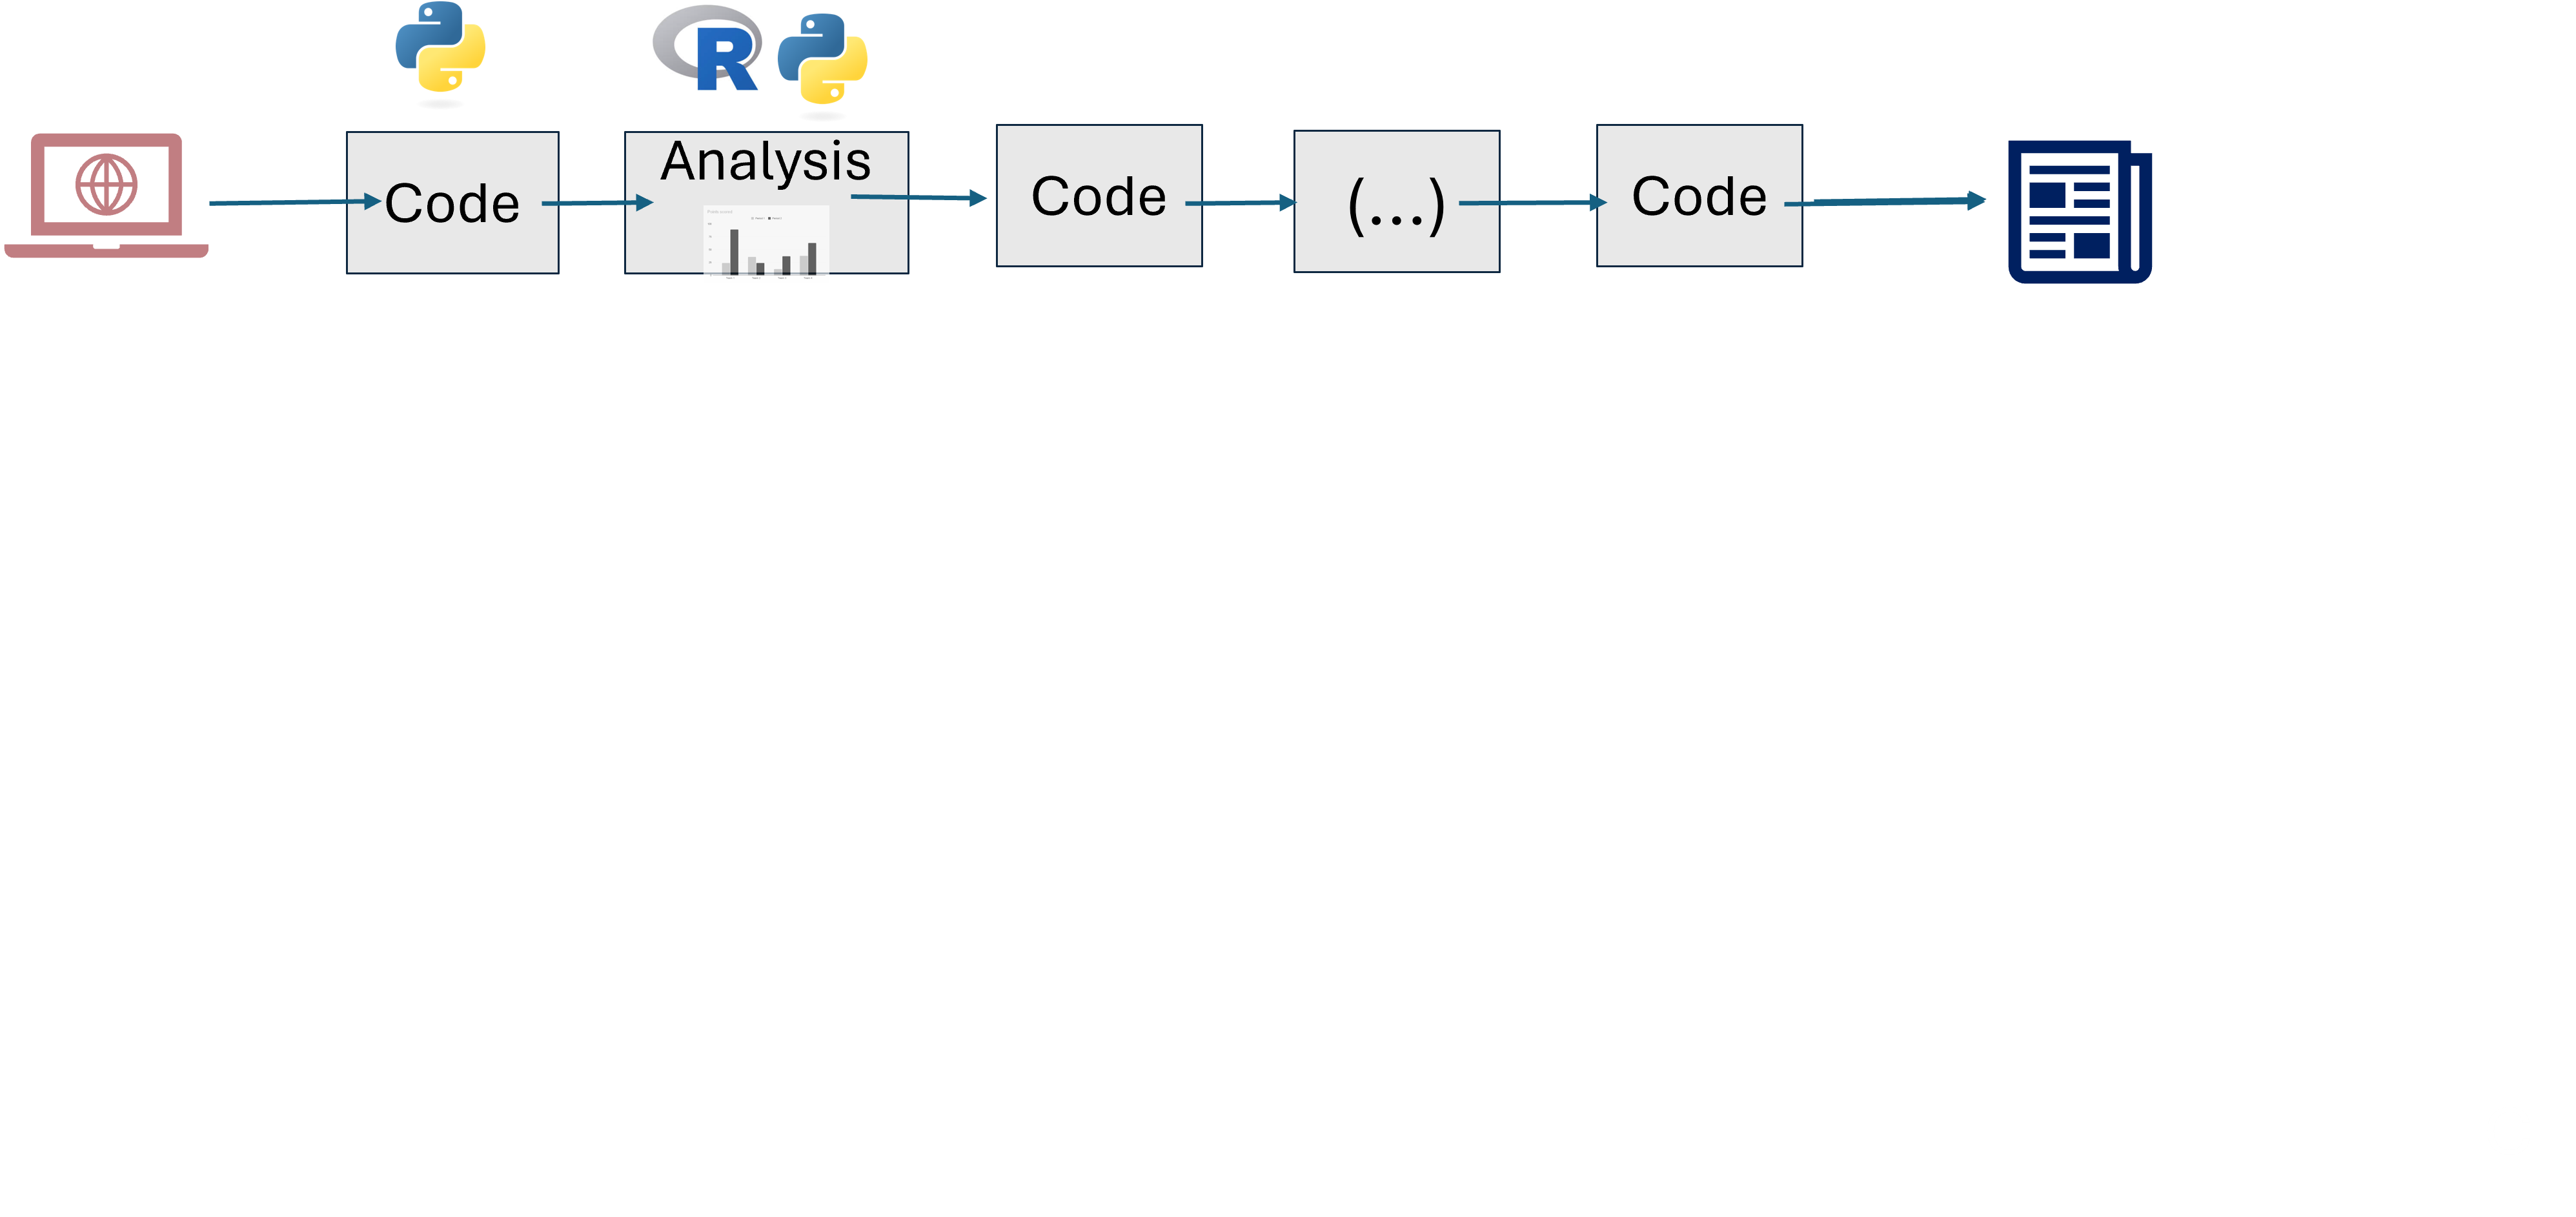
\includegraphics[width=0.8\textwidth]{Pipeline5.png} \\ Comment 5}
        \only<6>{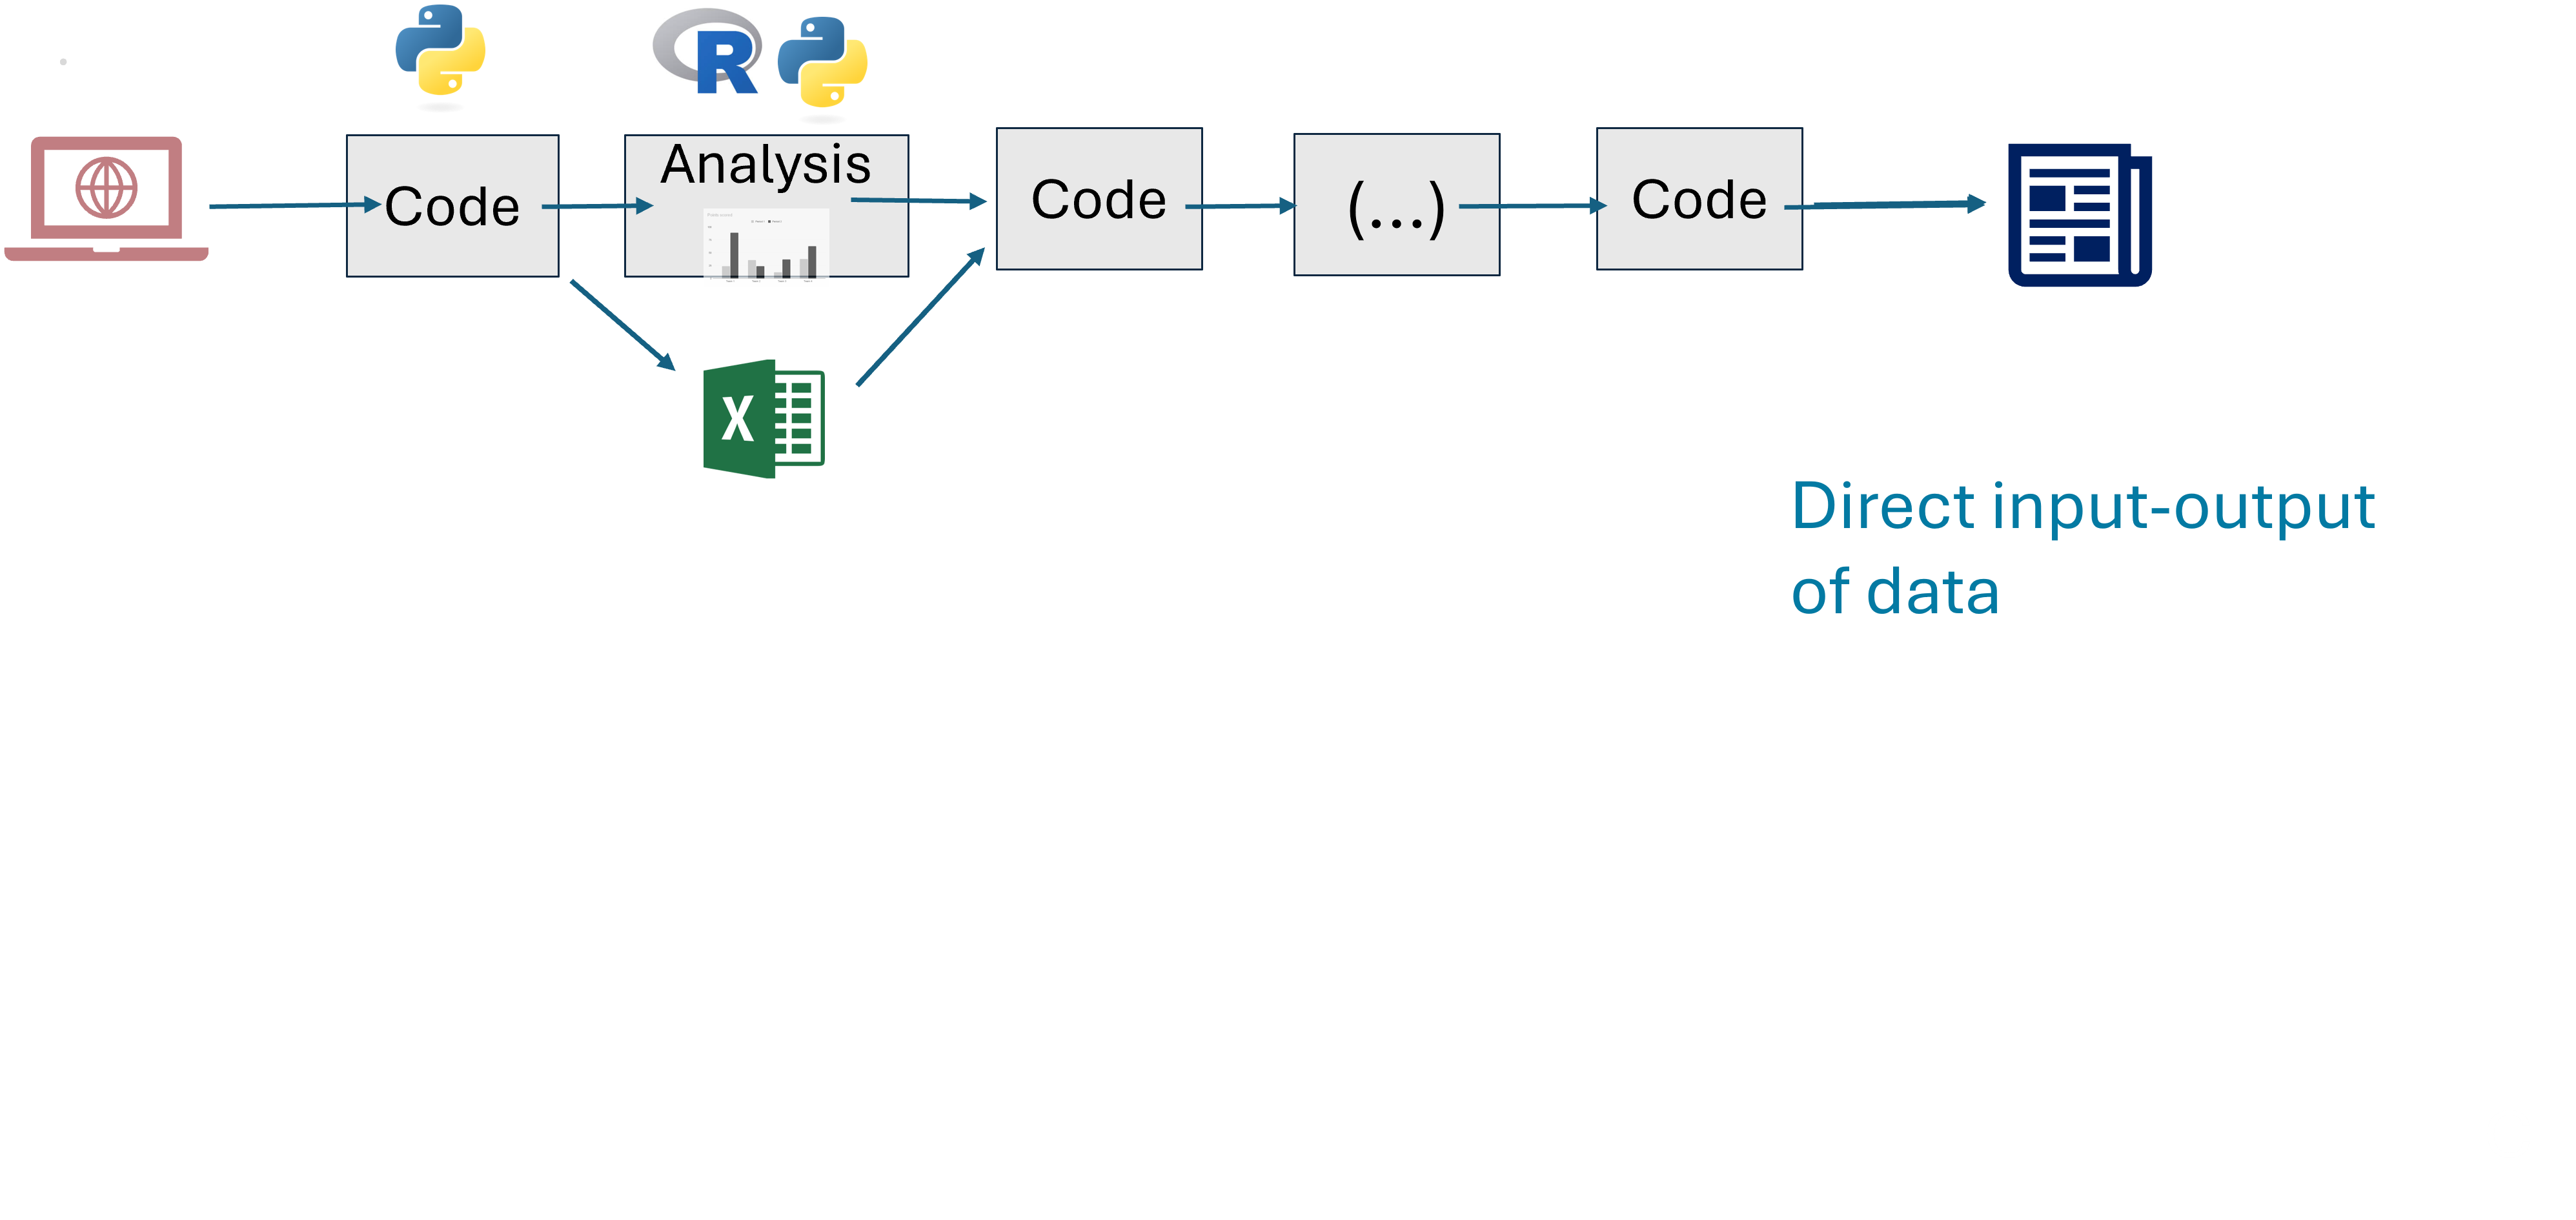
\includegraphics[width=0.8\textwidth]{Pipeline6.png} \\ Comment 6}
        \only<7>{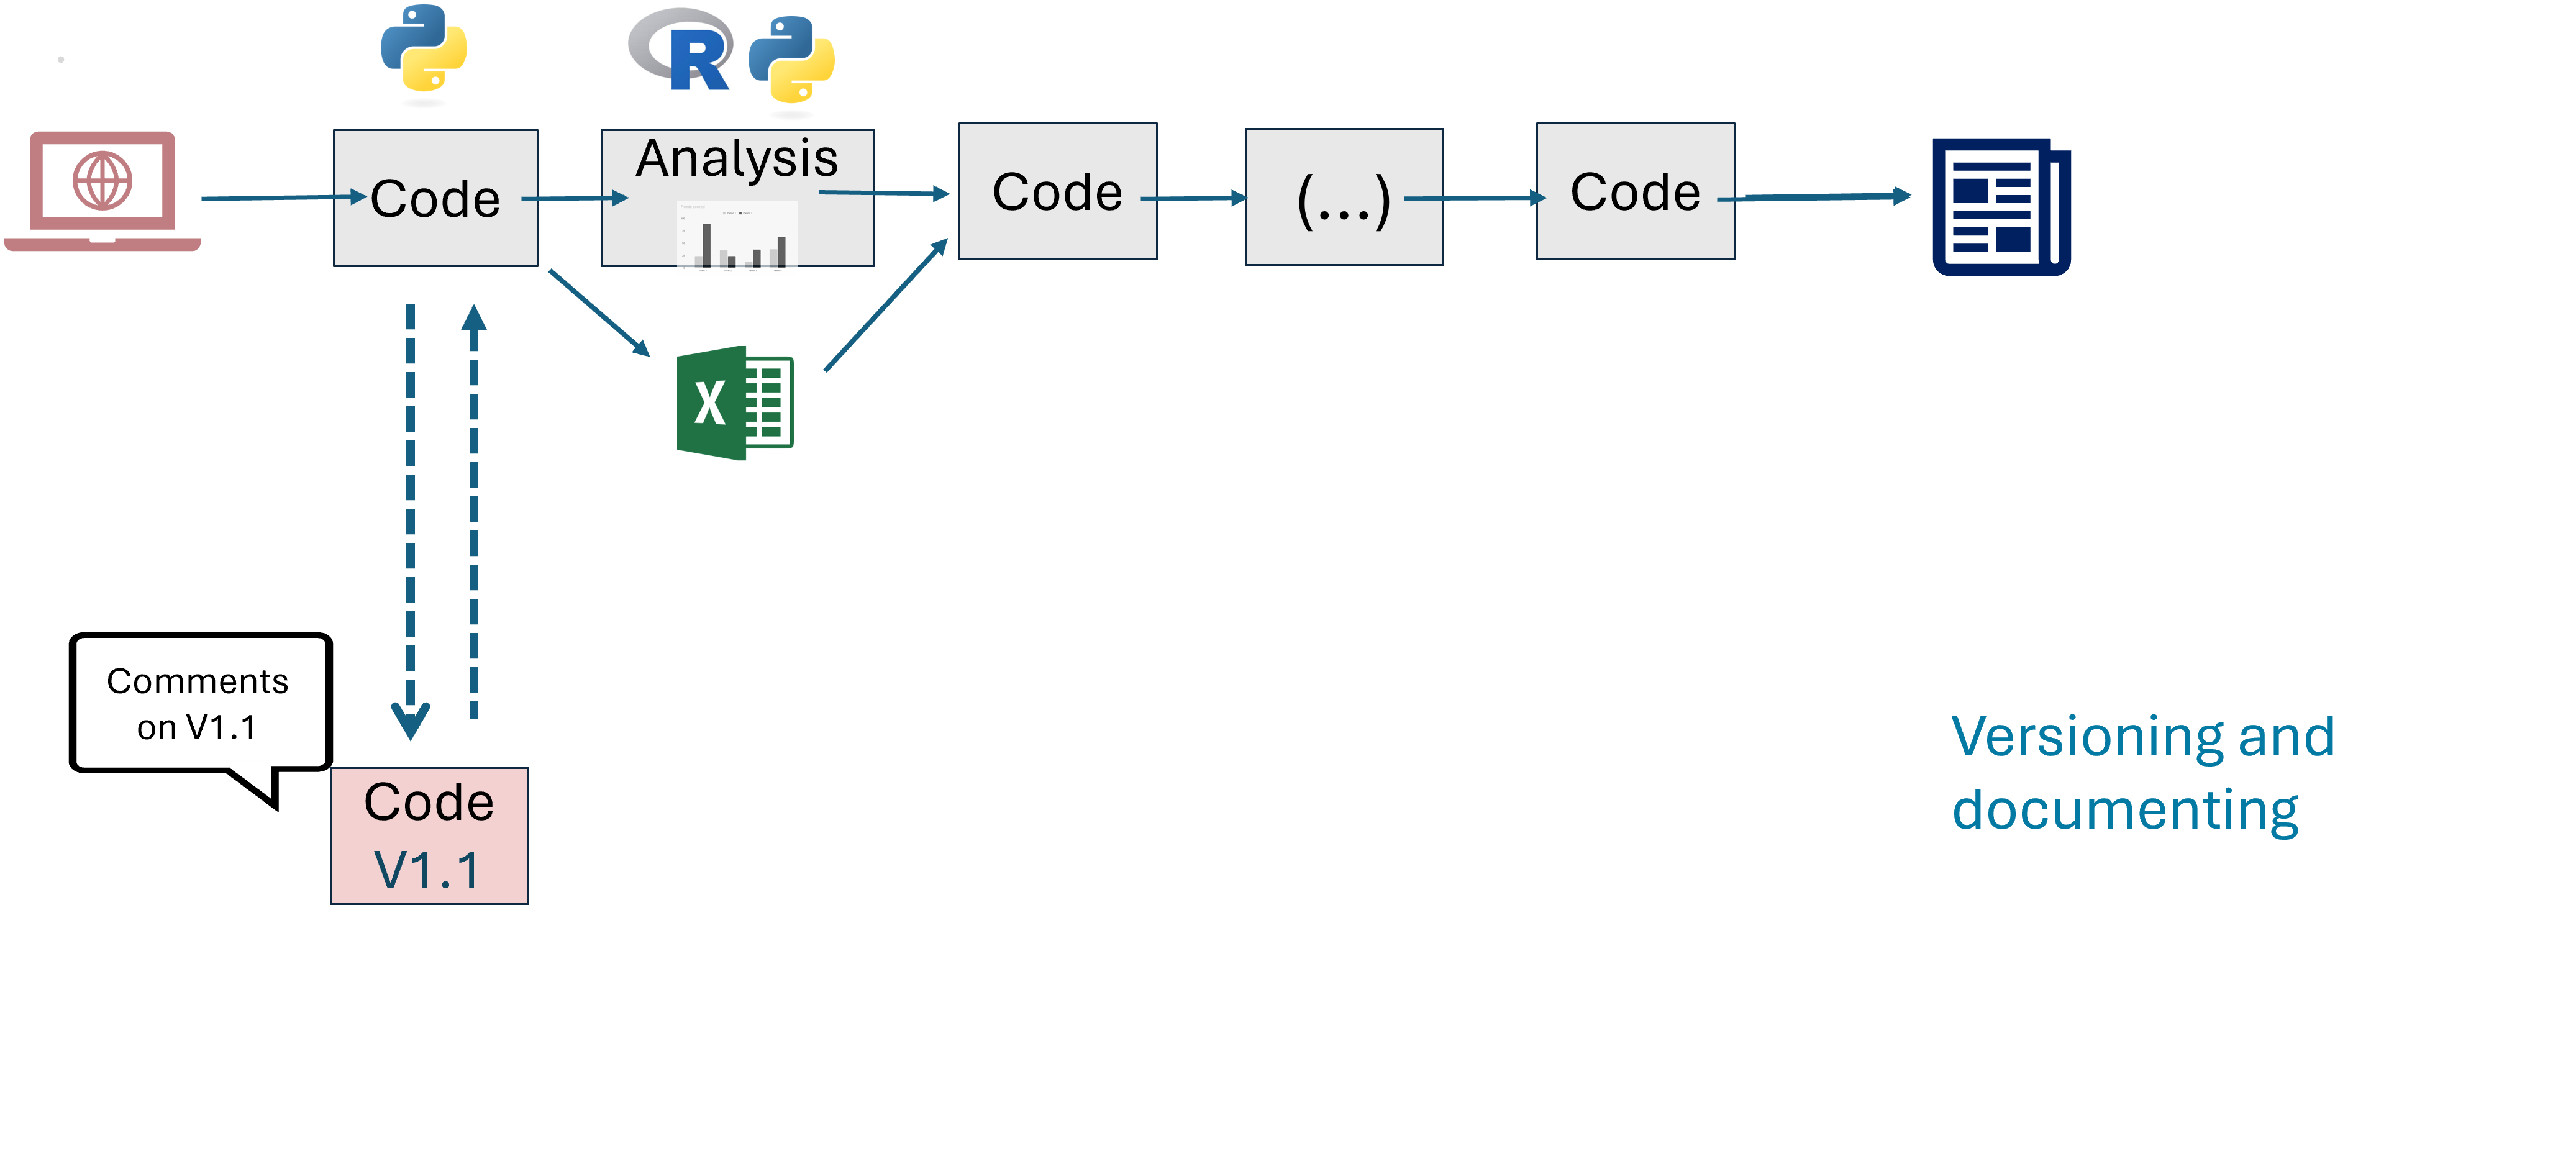
\includegraphics[width=0.8\textwidth]{Pipeline7.png} \\ Comment 7}
        \only<8>{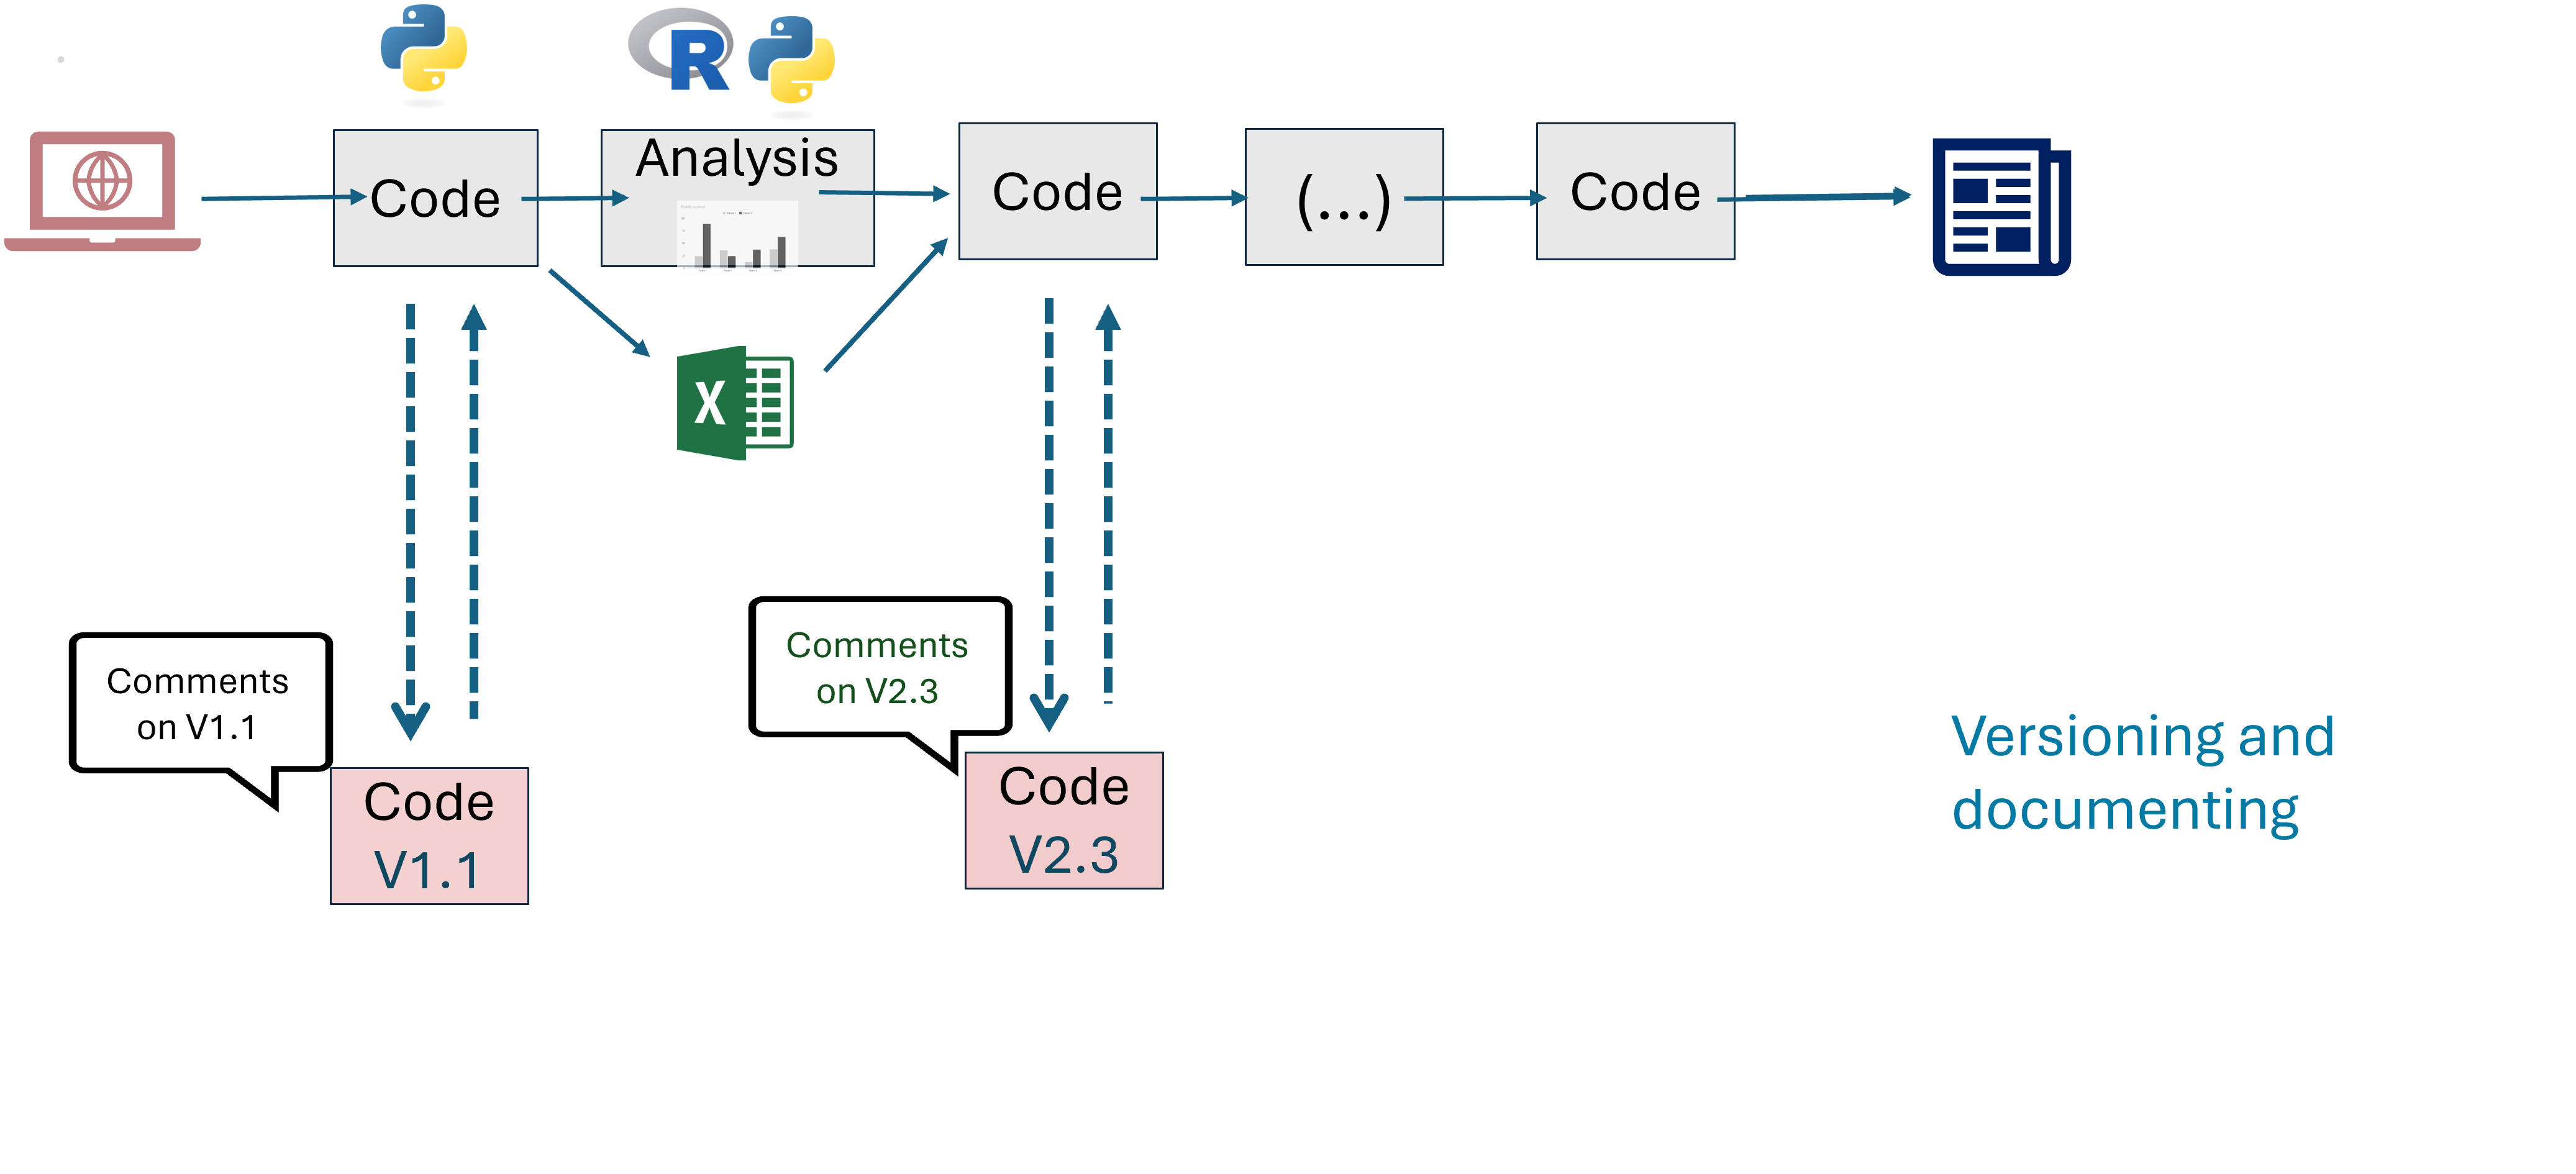
\includegraphics[width=0.8\textwidth]{Pipeline8.png} \\ Comment 8}
        \only<9>{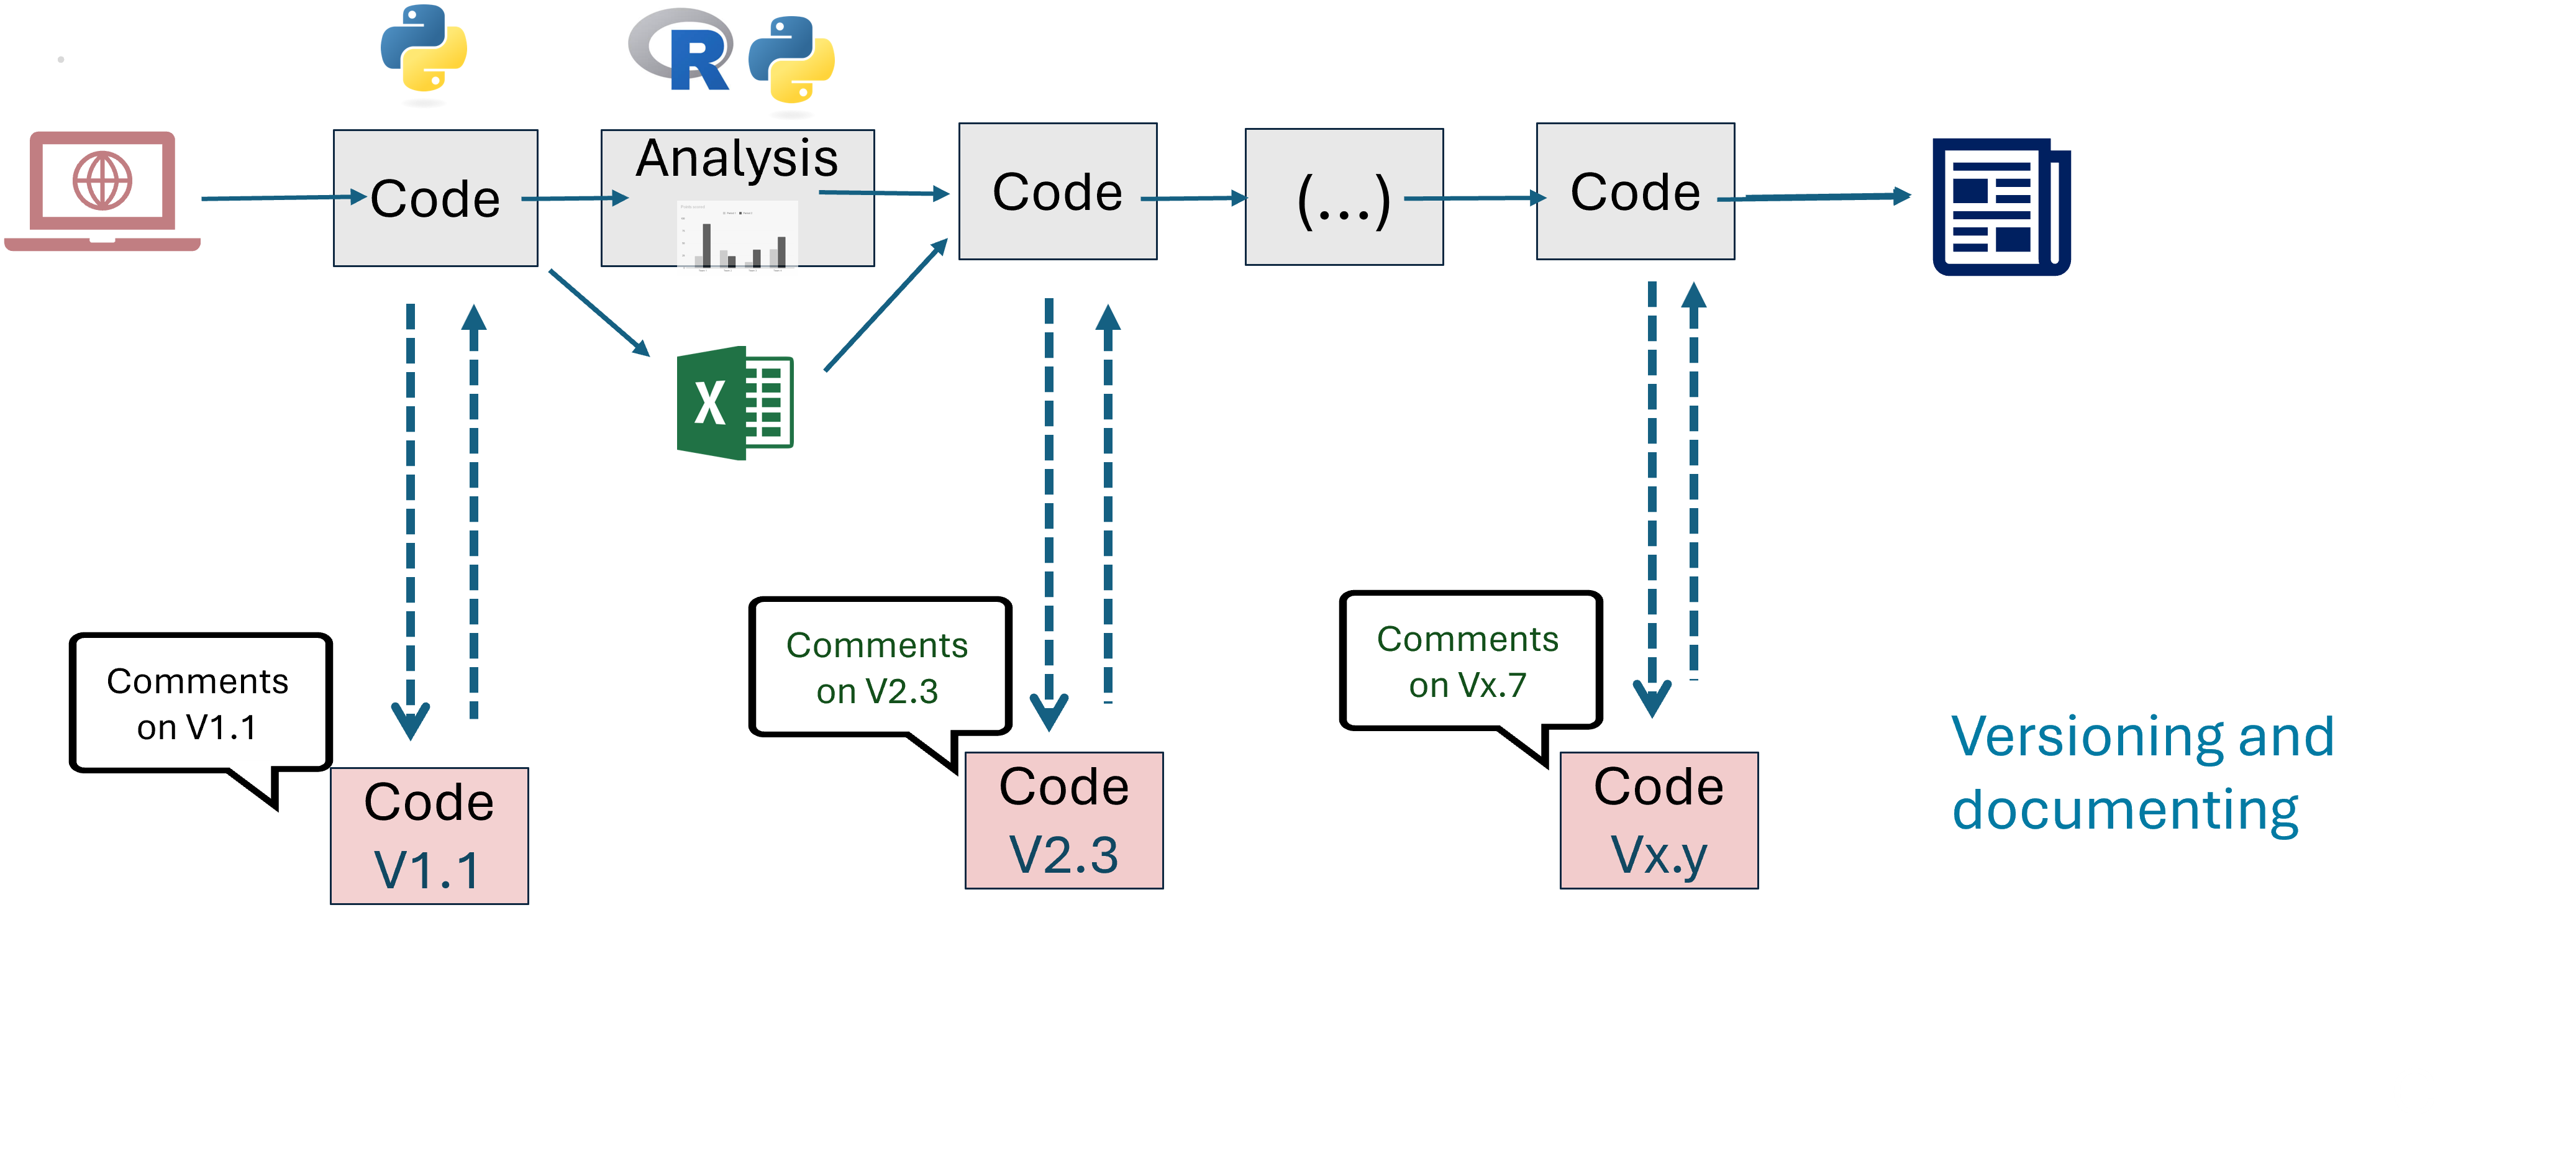
\includegraphics[width=0.8\textwidth]{Pipeline9.png} \\ Comment 9}
        \only<10>{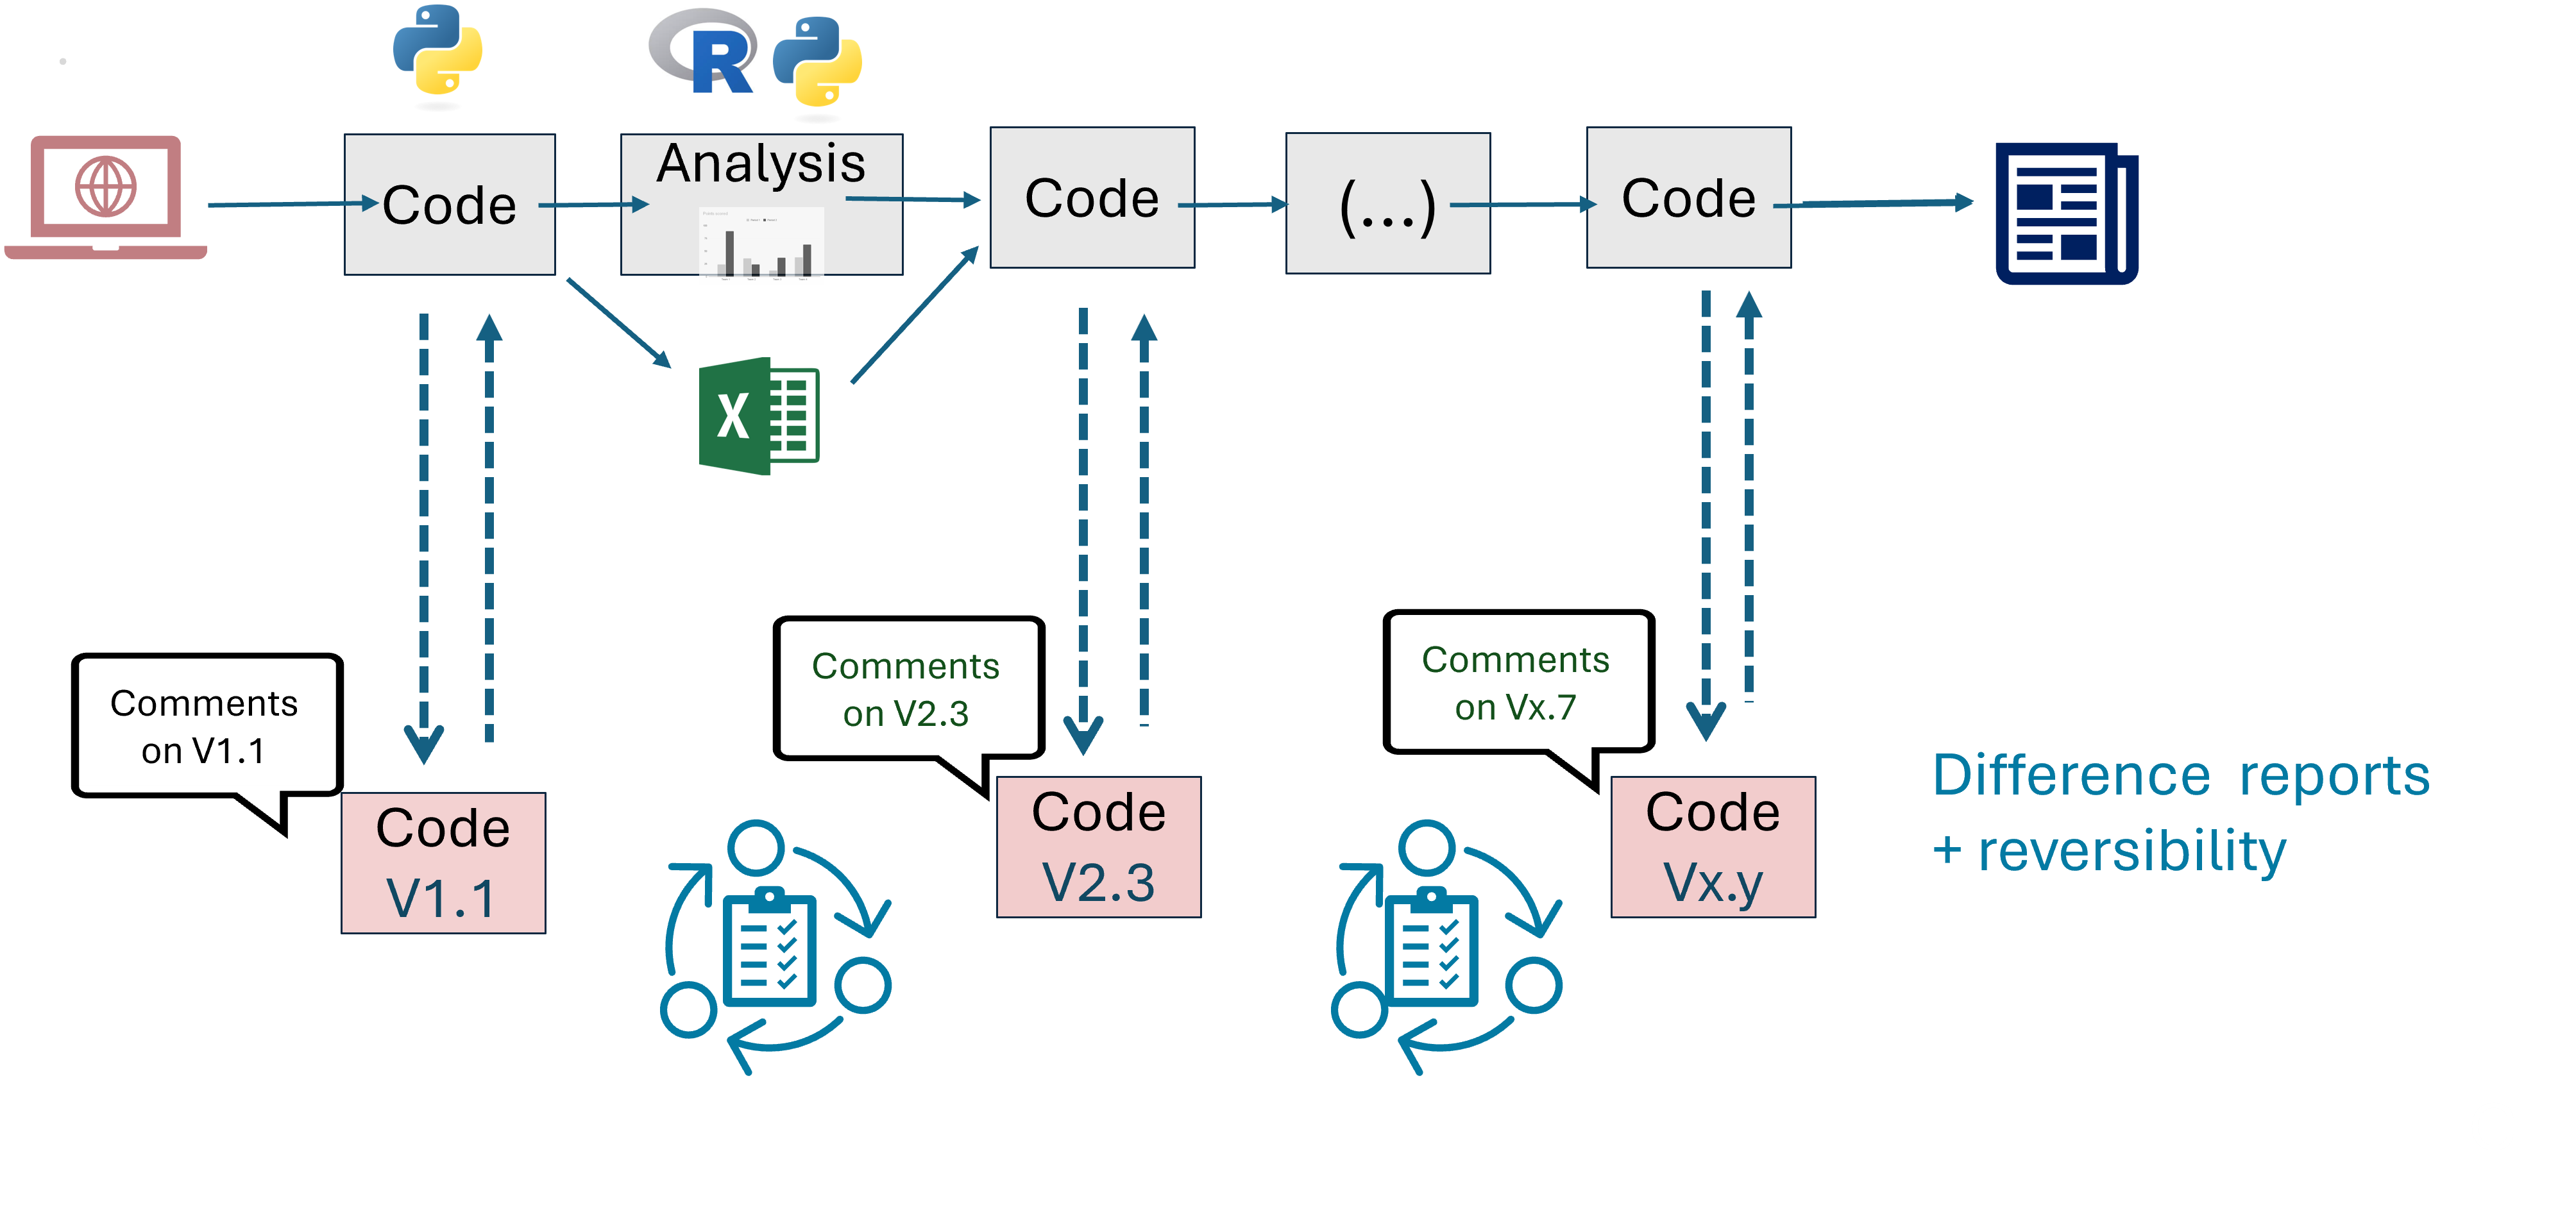
\includegraphics[width=0.8\textwidth]{Pipeline10.png} \\ Comment 10}
    \end{itemize}
\end{center}
\end{frame}


% Other slides go here...

\section{3 Principles}

\begin{frame}[<+->]
   \frametitle{3 main principles:}
    \begin{enumerate}
     \item Organize your work
     \item Code for others (including your future self)
     \item DRY: \textbf{D}o \textcolor{brique}{ not} \textbf{R}epeat \textbf{Y}ourself
      \item[]   \begin{alertblock}{}
            \begin{center}
                  \textit{Apply this in context (colleagues, code, software,...)}
            \end{center}
      \end{alertblock}
    \end{enumerate}
\end{frame}

\subsection{Organize your work }

\begin{frame}
\frametitle{Organize your work }
\textcolor{siap}{\textbf{Have a clear directory structure}}
 \pause
\begin{columns}[t]
 \begin{column}{0.4\textwidth}

    \begin{itemize}[<+->]
   \item Separate files into data, code, docs, etc.
   \item Make directories portable\\ (relative path)
    \end{itemize}
\end{column}
  \begin{column}{0.6\textwidth}
    \begin{center}
    \begin{itemize}
         \only<2-4>{ 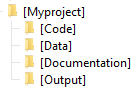
\includegraphics[width=0.5\textwidth]{WorkingDirectory.png} \\  }
         \only<2-4>{\hfill \tiny{ \textcolor{gris}{Example of a well-organized directory structure.}}\\ }
         \only<3-4>{\tiny{ \textbf{Usual}} \\ }
         \only<3-4>{ \tiny{mydata = pd.read\_csv("c://ESCAP/Webscraping/Data/WebData.csv")}  \\ \vspace{0.5cm} }
         \only<4>{\tiny{ \textbf{Better}}  \\}
         \only<4>{\tiny{\emph{Assuming your code is in } c://ESCAP/Webscraping/Code/ }  \\ }
         \only<4>{ \tiny{mydata = pd.read\_csv("../Data/WebData.csv")}  }

    \end{itemize}
    \end{center}
  \end{column}
\end{columns}
\end{frame}


\begin{frame}
\frametitle{Organize your work }
\textcolor{siap}{\textbf{Use naming conventions: } \\ }
For \textbf{files/code}\\
\begin{columns}[t]
 \begin{column}{0.3\textwidth}
    \begin{itemize}[<+->]
   \item Avoid  lazy names
   \item Meaningful files names
   \item Order of execution
    \end{itemize}
\end{column}
  \begin{column}{0.2\textwidth}
    \begin{itemize}
       \item[]
        \only<1-3>{ \small Usual \\ }
        \only<1-3>{ \small \texttt{prog1.ipynb}\\
                    \texttt{prog2.ipynb}\\
                    \texttt{Stat.ipynb}\\
                    \texttt{progC.ipynb}\\
                    \texttt{progP.ipynb} \\ }
    \end{itemize}
  \end{column}
  \begin{column}{0.5\textwidth}
    \begin{itemize}
        \item[]
        \only<2>{\small Better \\ }
        \only<2>{ \small    \texttt{Scraping\_Data.ipynb}\\
                            \texttt{Cleaning\_Data.ipynb}\\
                            \texttt{Stats\_Tables.ipynb}\\
                            \texttt{Classification.ipynb}\\
                            \texttt{Price\_CPI.ipynb} }
        \only<3>{\small Even better \\ }
        \only<3>{ \small
                    \texttt{01\_Scraping\_data.ipynb}\\
                    \texttt{02\_Cleaning\_data.ipynb}\\
                    \texttt{03\_Classification.ipynb}\\
                    \texttt{04\_Stats\_Tables.ipynb}\\
                    \texttt{04\_Price\_CPI.ipynb} }

    \end{itemize}
  \end{column}
\end{columns}
\end{frame}


\begin{frame}
\frametitle{Organize your work }
\textcolor{siap}{\textbf{Use naming conventions:} \\ }
For \textbf{outputs}
\begin{columns}[t]
 \begin{column}{0.3\textwidth}
    \begin{itemize}[<+->]
   \item Avoid numbering
   \item Explicit type of output
    \end{itemize}
\end{column}
  \begin{column}{0.2\textwidth}
    \begin{itemize}
    \item[]
        \only<1-2>{\small Usual \\ }
        \only<1-2>{\small \texttt{Table1.pdf} \\
                    \texttt{Table2.pdf} \\
                    \texttt{Graph.jpg} \\
                    \texttt{Model.csv} \\ }
    \end{itemize}
  \end{column}
  \begin{column}{0.5\textwidth}
    \begin{itemize}
    \item[]
        \only<2>{\small Better \\ }
        \only<2>{ \small  \texttt{Stat\_Desc\_Table.pdf} \\
                    \texttt{Price\_Stat\_Table.pdf}\\
                    \texttt{Dress\_Prices\_Graphic.jpg}\\
                    \texttt{All\_prices\_Results.csv} \\ }
    \end{itemize}
  \end{column}
\end{columns}
\end{frame}


\begin{frame}
\frametitle{Organize your work }
\textcolor{siap}{\textbf{Keep track of the workflow:} \\  }
 \begin{columns}[t]
 \begin{column}{0.5\textwidth}
    \begin{itemize}[<+->]
     \item Cut and paste should be avoided
     \item Every step of the process is coded
     \item Manage (and draw) the workflow
   \end{itemize}
  \end{column}
 \begin{column}{0.5\textwidth}
    \begin{itemize}
        \item[]
        \only<1-3>{ \includegraphics[width=1.0\textwidth]{Workflow.png} \\ }
        \only<1-3>{\hfill \tiny{ \textcolor{gris}{Example of a simple workflow.}} }
    \end{itemize}
  \end{column}
\end{columns}
\end{frame}



\begin{frame}
\frametitle{Organize your work }
\textcolor{siap}{\textbf{Use a version control system  (Git/GitHub)}} \\
\vspace{0.5cm}
\begin{center}
 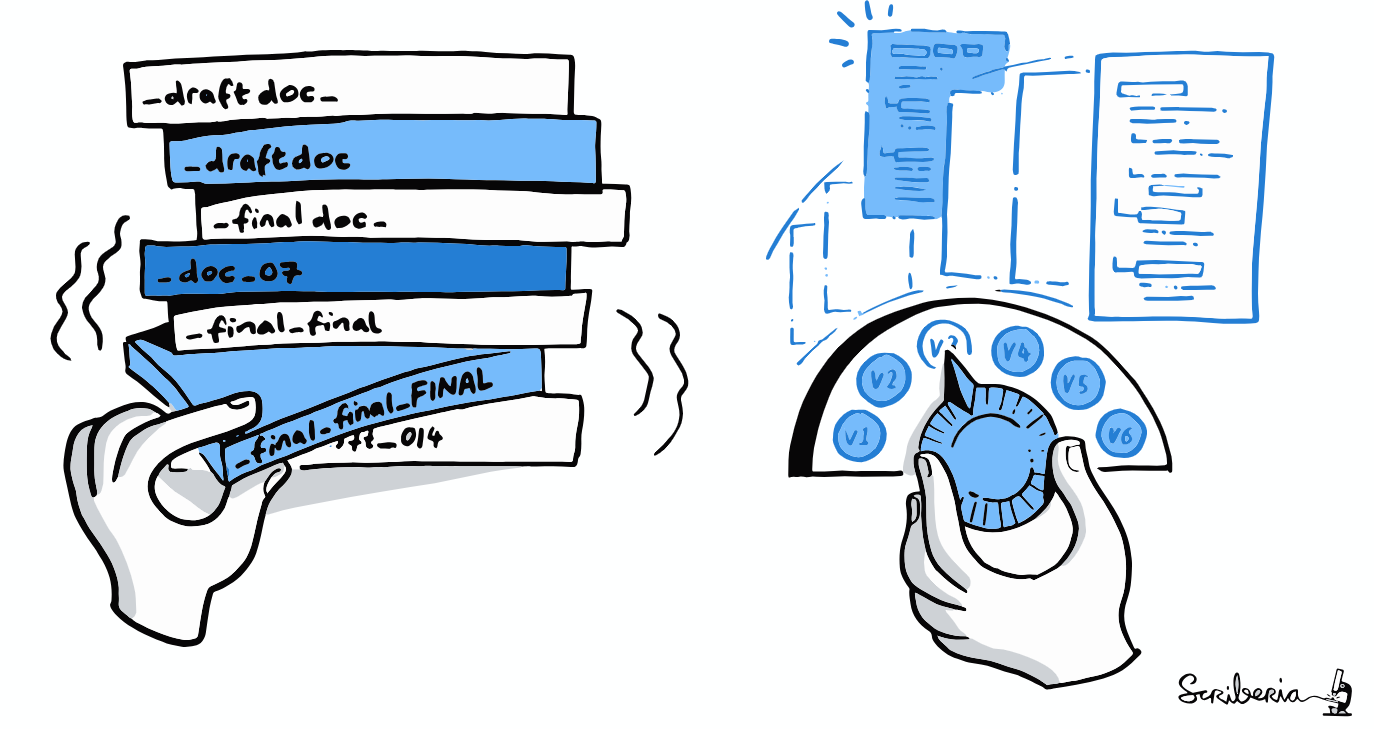
\includegraphics[width=0.7\textwidth]{FileHistory.PNG} \\

\large{\textbf{ More on Version Control later }}

\end{center}
\end{frame}

\subsection{Code for others}

\begin{frame}[<+->]
\frametitle{Code for others (including your "\emph{future self}")}
\textcolor{siap}{\textbf{Program with style:}} \\
          \begin{itemize}
             \item[]  \only<1>{Use \emph{literate programming} }
             \only<1>{ \begin{center}
                    ``\textit{Let us concentrate rather on explaining to humans \\ what we want the computer to do}'' \\
                    \hfill \textcolor{gris}{ D. Knuth (1984)}
             \end{center}}

             \only<2>{ \begin{center}
                    ``\textit{($\cdots$) code is read much more often than it is written}''  \\
                    \hfill \textcolor{gris}{  \href{https://peps.python.org/pep-0008/}{Guido van Rossum (2013 -PEP8)}    \\
                     \vfill \hfill \footnotesize{\href{https://peps.python.org/pep-0000/}{PEP stands for \emph{Python Enhancement Proposals}}}}
             \end{center}}

             \only<3>{ Use conventions on layout (Comments, indentation,...)  \\
             \href{https://peps.python.org/pep-0008/}{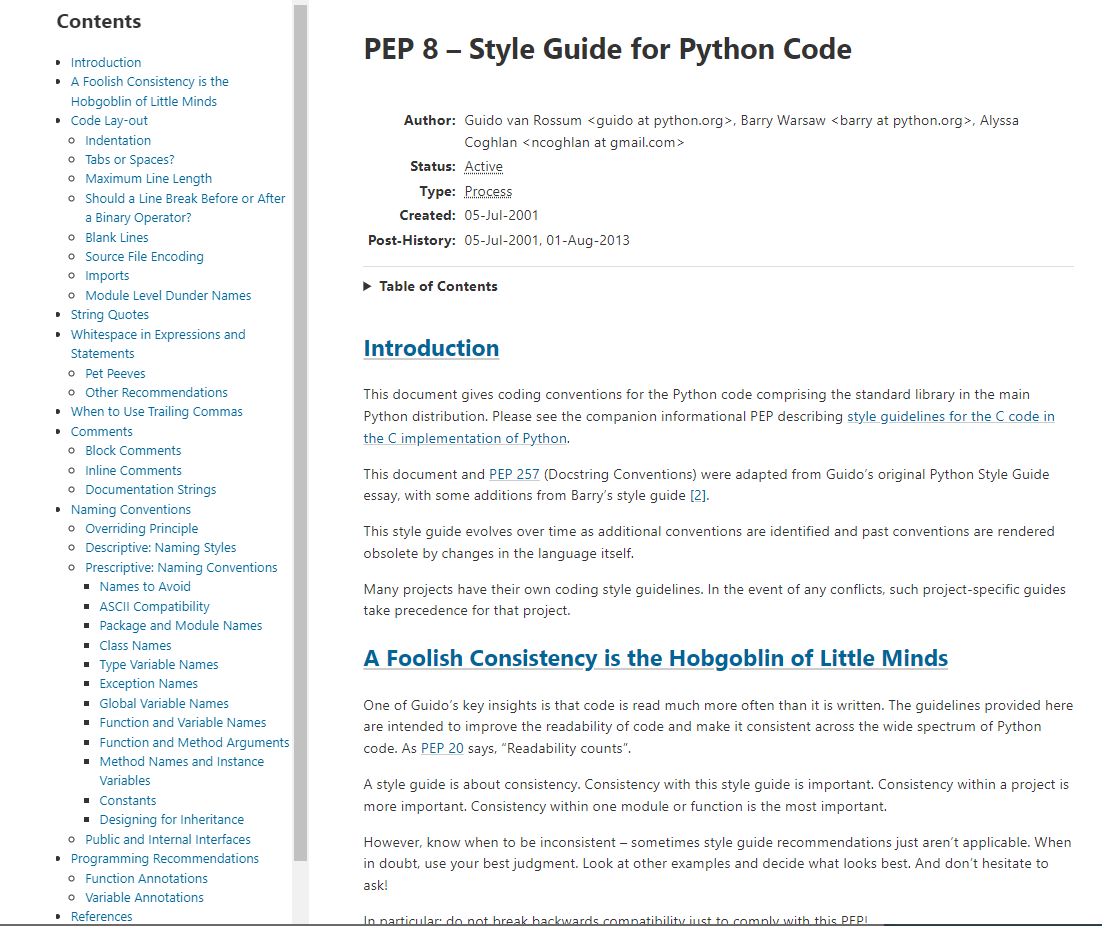
\includegraphics[width=0.8\textwidth]{PEP8-Style.png}}}
         \end{itemize}
\end{frame}


\begin{frame}
\frametitle{Code for others }
\textcolor{siap}{\textbf{Program with style}} \\
\begin{columns}[t]
 \begin{column}{0.3\textwidth}
    \begin{itemize}[<+->]
   \item Avoid ambiguities
   \item Avoid changing units
    \end{itemize}
\end{column}
  \begin{column}{0.7\textwidth}
    \begin{itemize}
    \item[]
        \only<1>{\scriptsize Usual \\ }
        \only<1>{\scriptsize \texttt{df['sex'] = np.where(df['gender'] == '1001', 1, 2)} \\}
        \only<1>{\small Better \\ }
        \only<1>{\scriptsize \texttt{df['female'] = np.where(df['gender'] == '1001', 1, 0)} \\
                                 \texttt{df['male'] = np.where(df['gender'] != '1001', 1, 0)} \\ }
         \only<2-4>{\scriptsize Usual \\ }
        \only<2-4>{\scriptsize \texttt{df['gdp'] = df['gdp'] / 118.722 } \\
                                \texttt{ } \\ }
        \only<3>{\scriptsize Better \\ }
        \only<3>{\scriptsize \texttt{df['gdp\_US'] = df['gdp'] / 118.722} }
        \only<4>{\scriptsize Even better \\ }
        \only<4>{\scriptsize \texttt{US\_Vanu\_exch\_rate = 118.722} \\
                                 \texttt{df['gdp\_US'] = df['gdp']/ US\_Vanu\_exch\_rate}  }

    \end{itemize}
  \end{column}
\end{columns}
\end{frame}

%\end{document}

%%%%%%
\subsection{DRY}
\begin{frame}
\frametitle{\textbf{D}o not \textbf{R}epeat \textbf{Y}ourself  }

\textcolor{siap}{\textbf{Create reusable objects}} \\
\begin{columns}[t]
 \begin{column}{0.2\textwidth}
    \begin{itemize}[<+->]
       \item { \scriptsize Store values}
       \item[]{ \scriptsize Avoid repetitions}
        \item[]
       \item { \scriptsize Use functions}
    \end{itemize}
\end{column}
  \begin{column}{0.8\textwidth}
    \begin{itemize}
    \item[]
        \only<1-2>{\scriptsize Usual \\ }
        \only<1-2>{\scriptsize \texttt{Current\_Data = Mydata[Mydata['year'] == 2023]} \\
                               \texttt{ } \\ }
        \only<2>{\scriptsize Better \\ }
        \only<2>{\scriptsize \texttt{Current\_year = 2023 } \\
                        \texttt{Current\_Data= Mydata[Mydata['year'] } \\
                       \hfill  \texttt{== Current\_year] } }
        \only<3>{\scriptsize Usual \\ }
        \only<3>{\scriptsize \texttt{data = Mydata[Mydata['export'] == 'Beef']} \\
                 \scriptsize \texttt{plt.plot(data['Year'], data['Value'])} \\
                 \scriptsize \texttt{plt.title('Export for Beef')\\ } \\
                  \texttt{ } \\  }
         \only<3>{\scriptsize \texttt{data = Mydata[Mydata['export'] == 'Kava']} \\
                 \scriptsize \texttt{plt.plot(data['Year'], data['Value'])} \\
                 \scriptsize \texttt{plt.title('Export for Kava')} \\
                 \texttt{ ... } \\ }
        \only<4>{\scriptsize Better \\ }
        \only<4>{\scriptsize \texttt{def plot\_export(export\_type): } \\
                                \texttt{     data = Mydata[Mydata['export'] }  \\
                                \hfill \texttt{== export\_type]} \\
                                \texttt{     plt.plot(data['Year'], data['Value'])}\\
                                \texttt{     plt.title(f'Export for {export\_type}')} \\
                                \texttt{     plt.show()}\\
                                \texttt{ } \\
                                \texttt{plot\_export("Beef")} \\
                                \texttt{plot\_export("Kava")   }}

    \end{itemize}
  \end{column}
\end{columns}
\end{frame}


\begin{frame}
\frametitle{Other principles}
    \begin{itemize}[<+->]
        \item Discuss with colleagues that may use your work
        \item Automatize as much as you can
        \item[$\hookrightarrow$] Reduces your brain's memory burden
        \item There are easy steps everybody can do
        \item[$\hookrightarrow$] Write small programs, one for each task
        \item Use open source program
        \item[$\hookrightarrow$] Easier to share, easier to automatize
        \item[$\hookrightarrow$] Also cost-effective
        \item Test your work regularly:
        \only<11>{\begin{center}
            \emph{``Do what has been said, say what has been done, and \\ check that what has been said has really been done !''}
         \end{center}}
        \only<12>{\begin{center}
            \emph{``\textbf{Code} what has been said, say what has been \textbf{coded}, and \\ check that what has been said has really been \textbf{coded}  !''}
         \end{center}}
    \end{itemize}
\end{frame}


\section{Version Control}

\begin{frame} % Cover slide
\frametitle{Version Control keeps tracks of your work}
Tracking three \textbf{W} questions:
\begin{columns}[t]
 \begin{column}{0.5\textwidth}
 \begin{itemize}[<+->]
 \item[] \textcolor{siap}{\textbf{W}}hat changes?
 \item[] \textcolor{siap}{\textbf{W}}ho made the changes?
 \item[] \textcolor{siap}{\textbf{W}}hen were the changes made?
 \end{itemize}
 \end{column}
  \begin{column}{0.5\textwidth}
    \begin{center}
    \begin{itemize}
        \only<1-4>{ 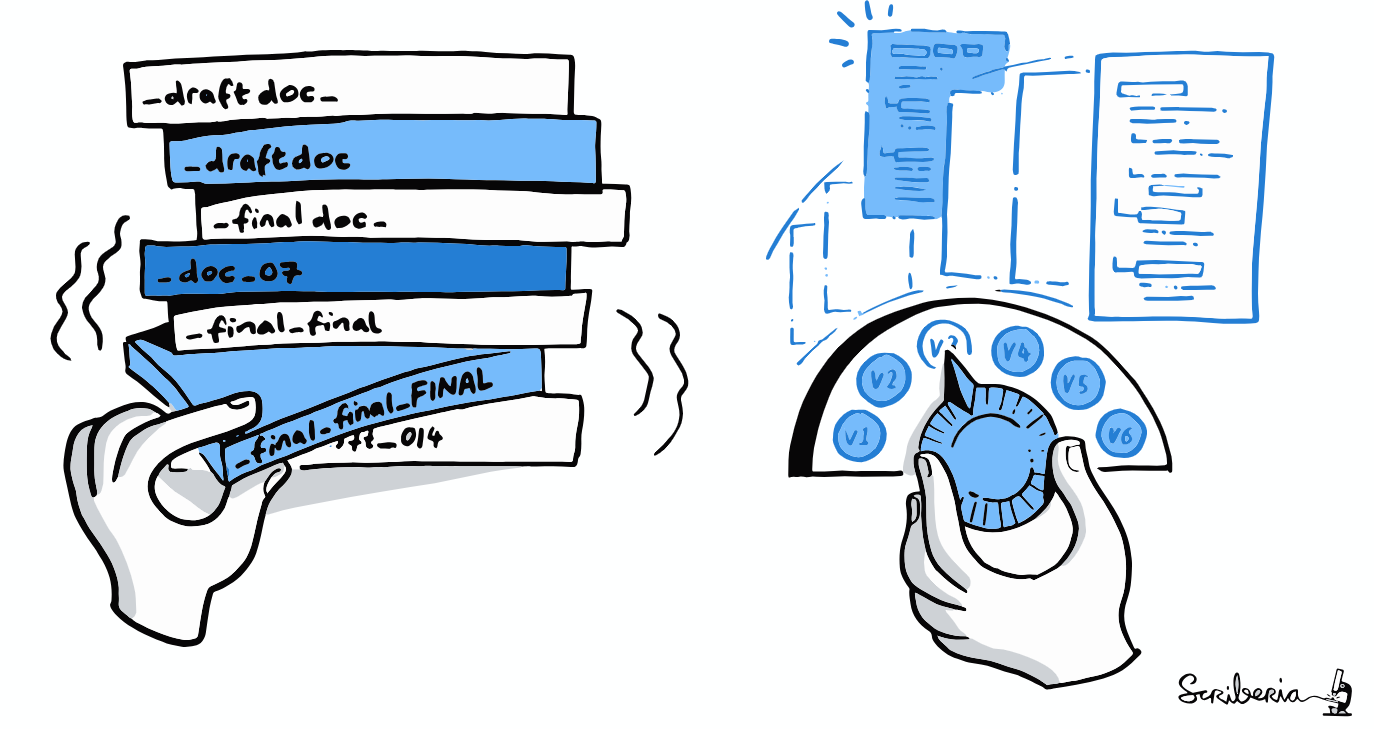
\includegraphics[width=0.95\textwidth]{FileHistory.PNG} \\  }
       \only<1-4>{\hfill  \textcolor{gris}{\tiny{Source: \href{https://the-turing-way.netlify.app/reproducible-research/vcs.html}{The Turing Way project}}}}
    \end{itemize}
    \end{center}
  \end{column}
\end{columns}
\end{frame}



\begin{frame}{Transparency, Accountability \& Reproducibility}
    \begin{itemize}[<+->]
        \item Version control provides a detailed history of changes
        \item Each modification is attributed to a specific user
        \item Promotes accountability, transparency \&  reproducibility
    \end{itemize}
\end{frame}

\subsection{File evolution}

\begin{frame}{The evolution of a file \textcolor[rgb]{1.00,0.00,0.00}{\textbf{<--XXXX To revise this}} }
\begin{center}
\begin{itemize}
   \only<1> {
\includegraphics[width = 1.0\textwidth]{FileChange1a.png} \\ }
   \only<2> {
\includegraphics[width = 1.0\textwidth]{FileChange2a.png} \\ }
   \only<3> {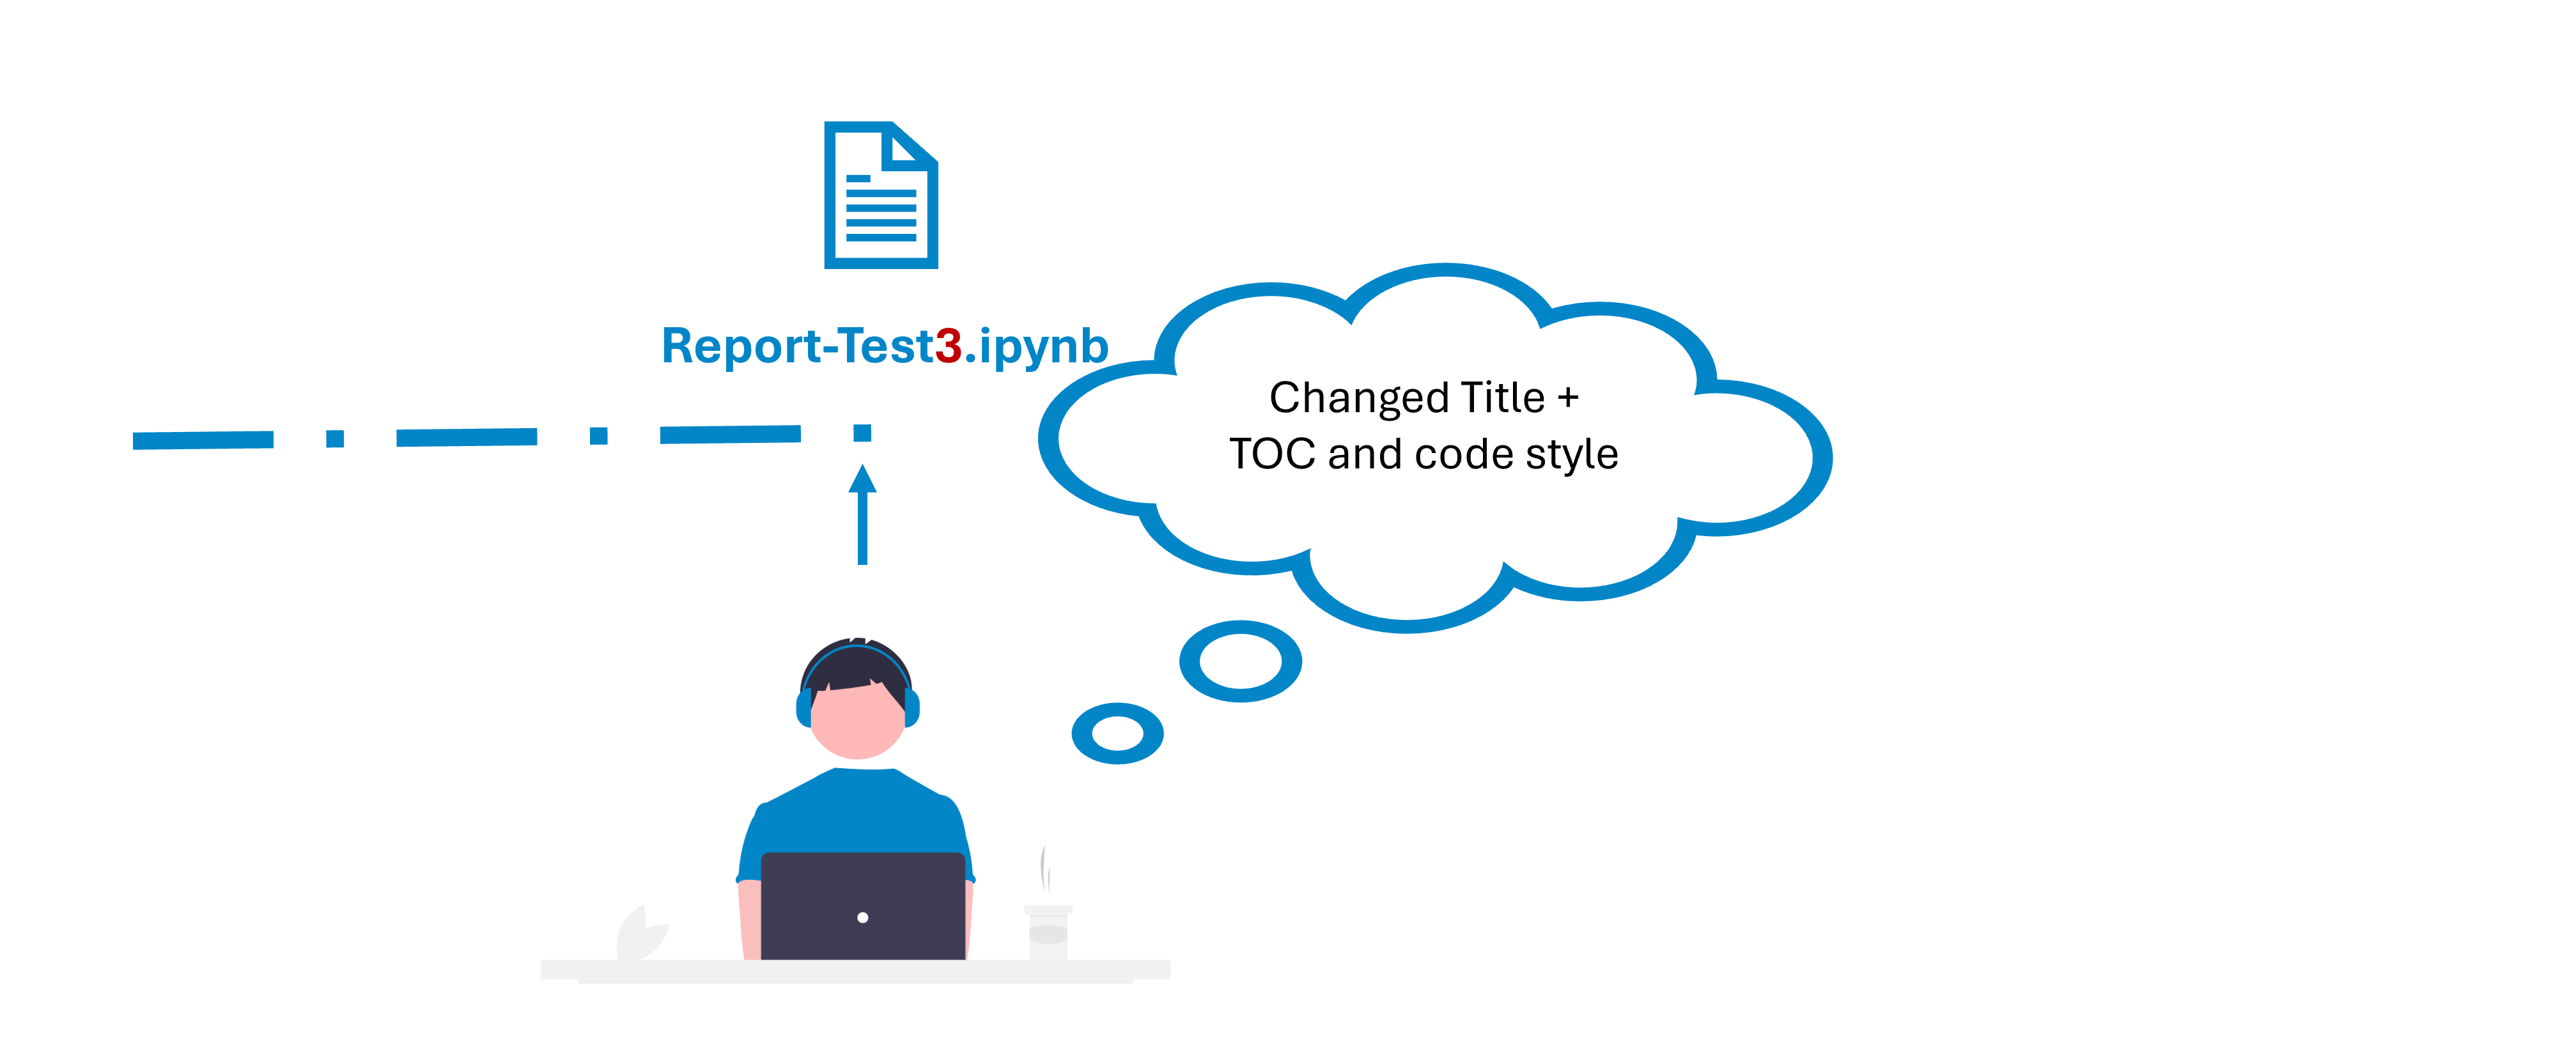
\includegraphics[width = 1.0\textwidth]{FileChange3a.png} \\ }
   \only<4> {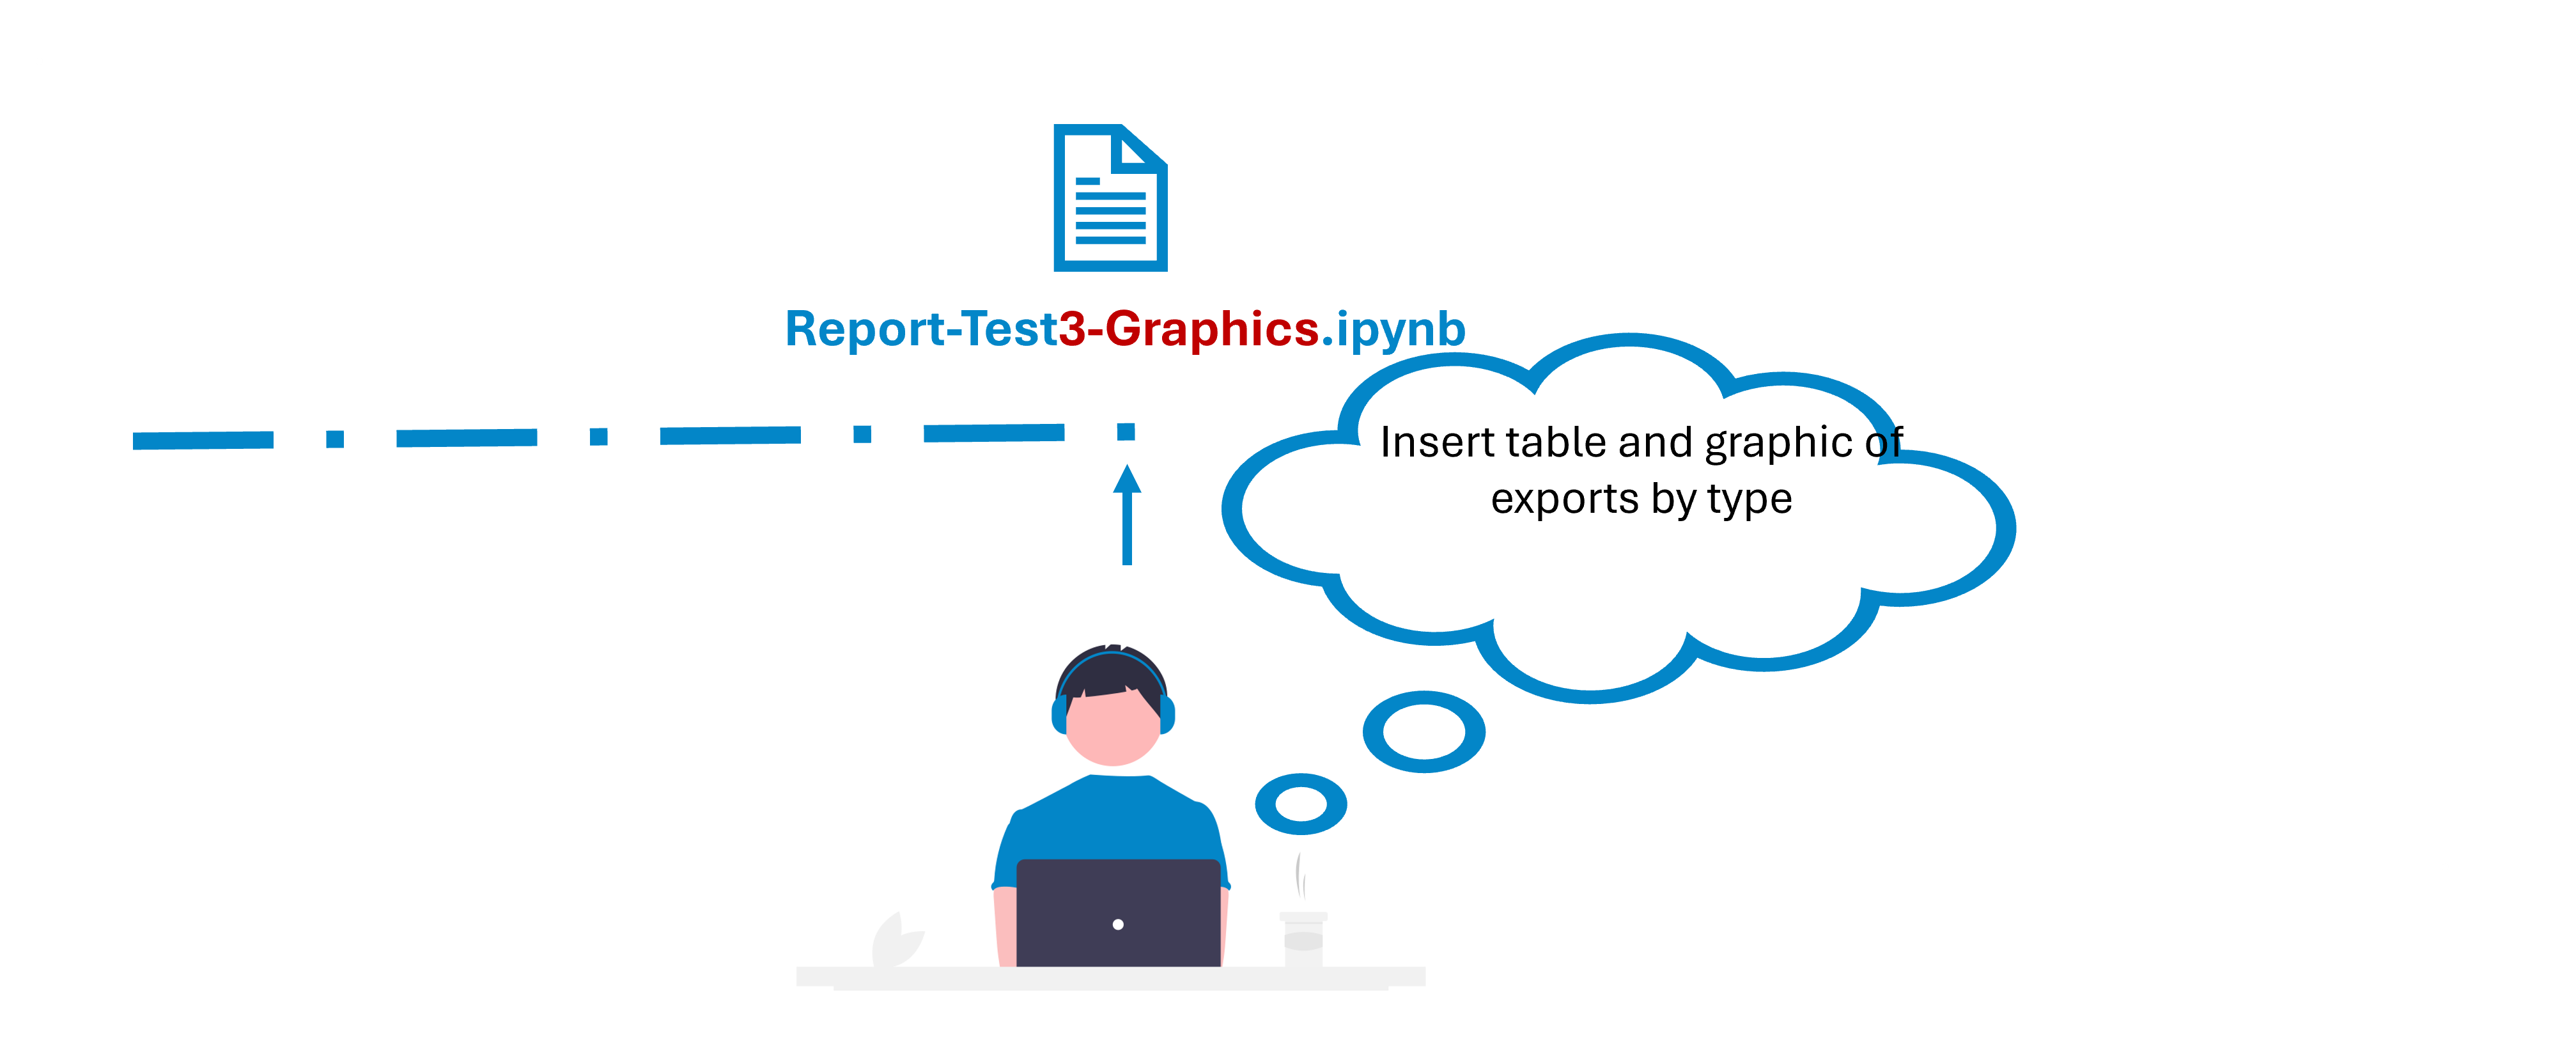
\includegraphics[width = 1.0\textwidth]{FileChange4a.png} \\ }
   \only<5> {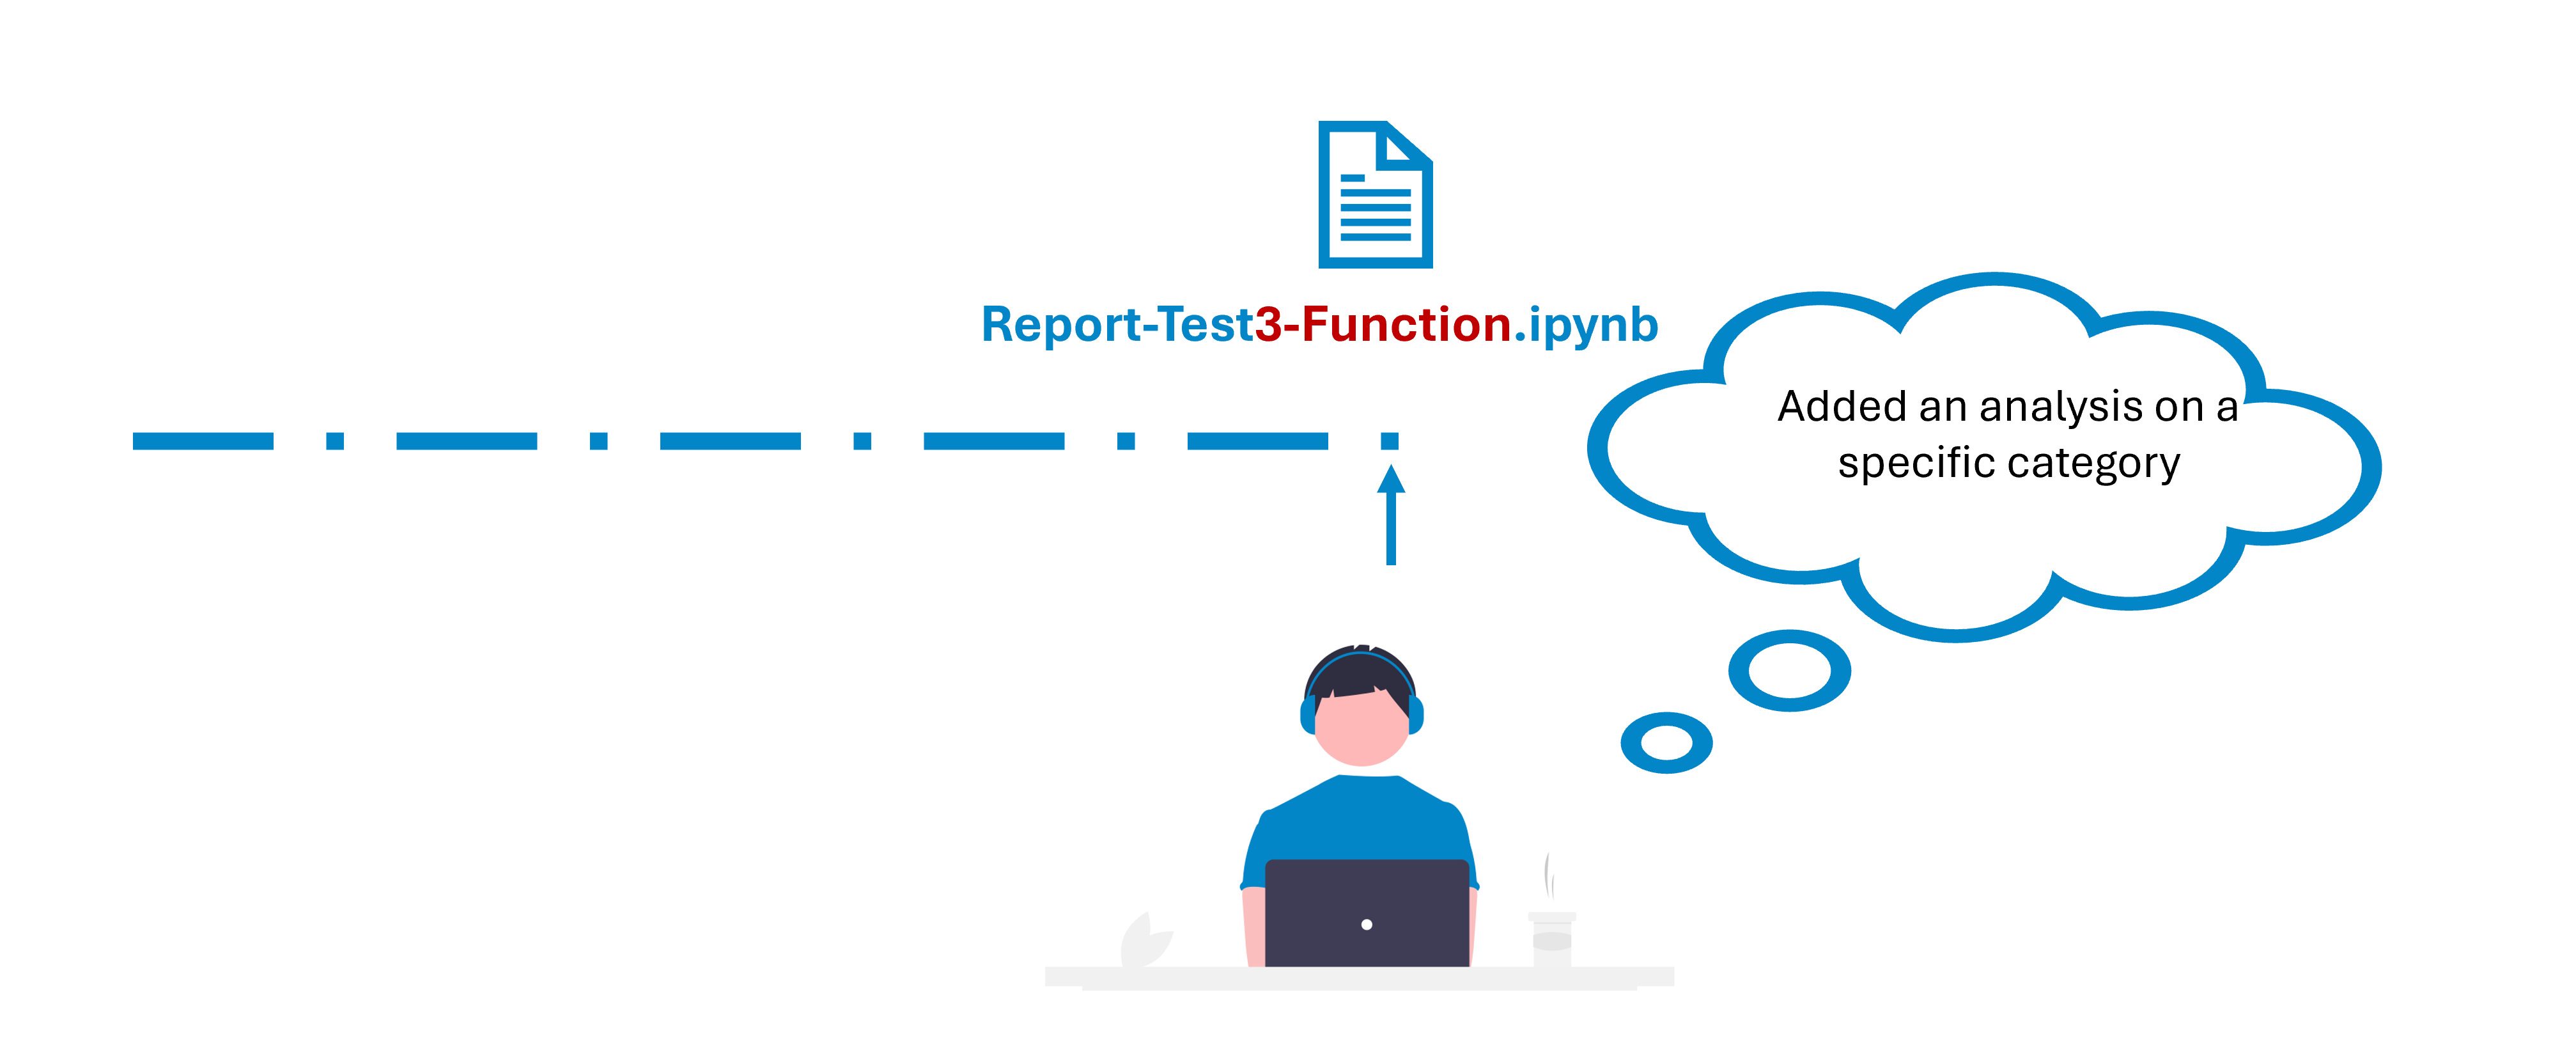
\includegraphics[width = 1.0\textwidth]{FileChange5a.png} \\ }
   \only<6> {\includegraphics[width = 1.0\textwidth]{FileChange6a.png} \\ }
   \only<7> {\includegraphics[width = 1.0\textwidth]{FileChange7a.png} \\ }
\end{itemize}
\end{center}
\end{frame}

\begin{frame}{The evolution of a file  \textcolor[rgb]{1.00,0.00,0.00}{\textbf{<--XXXX To revise this}} }
Usual ways to keep track of changes:
\pause
\begin{columns}[t]
\begin{column}{0.6\textwidth}
\begin{itemize}[<+->]
        \item New file after each change
        \item[$\hookrightarrow$] Need to open each file to see the change
        \item[$\hookrightarrow$] Names have to be explicit
        \item Only the last file with lots of comments
        \item Not fulfilling the 3 \textcolor{siap}{\textbf{W}}...

    \end{itemize}
 \end{column}
  \begin{column}{0.4\textwidth}
    \begin{center}
    \begin{itemize}
        \only<1-4>{ \includegraphics[width=1.0\textwidth]{FileLifeAll.png} \\  }
        \only<5-6>{ \includegraphics[width=0.95\textwidth]{FileLifeFinalFinal.png} \\  }
       % \only<7>{ \includegraphics[width=1.0\textwidth]{FileLifeAll.png} \\  }
       % \only<7>{\hfill \includegraphics[width=0.5\textwidth]{FileLifeFinalFinal.png} \\  }

    \end{itemize}
    \end{center}
  \end{column}
\end{columns}
\end{frame}

\subsection{Main Commands}

\begin{frame}{The evolution \textcolor{brique}{with Version Control}}
Record a message (\emph{commit})  for each change!
\begin{center}
\begin{itemize}
   \only<1> {\includegraphics[width = 1.0\textwidth]{FileLife1.png} \\ }
   \only<2> {\includegraphics[width = 1.0\textwidth]{FileLife2.png} \\ }
   \only<3> {\includegraphics[width = 1.0\textwidth]{FileLife3.png} \\ }
   \only<4> {\includegraphics[width = 1.0\textwidth]{FileLife4.png} \\ }
   \only<5> {\includegraphics[width = 1.0\textwidth]{FileLife5.png} \\ }
   \only<6> {\includegraphics[width = 1.0\textwidth]{FileLife6.png} \\ }
   \only<7> {\includegraphics[width = 1.0\textwidth]{FileLife7.png} \\ }
\end{itemize}
\end{center}
\end{frame}

\begin{frame}{The history of the file is recorded!}
\begin{center}
\begin{itemize}
   \only<1-2> {Each version is documented (with \emph{commits}) \\ }
   \only<1-2> {\includegraphics[width = 1.0\textwidth]{FileLifeHistoryEnd.png} \\ }
   \only<3-4> {Each version embeds the full history!  }
   \only<3-4> {\includegraphics[width = 1.0\textwidth]{FileLifeHistoryFull.png} \\ }
\end{itemize}
\end{center}
\end{frame}

\begin{frame}{Going back and "undo" is possible}
\begin{center}
\begin{itemize}
   \only<1-2> {It is possible to review previous version... \\ }
   \only<1-2> {\includegraphics[width = 1.0\textwidth]{FileLifeBack.png} \\ }
   \only<3-4> {...to compare the changes...  }
   \only<3-4> {\includegraphics[width = 1.0\textwidth]{FileLifeDiff.png} \\ }
   \only<5-6> {... and to revert  to a  previous version... }
   \only<5-6> {\includegraphics[width = 1.0\textwidth]{FileLifeRevert.png} \\ }
   \only<7-8> {... or \emph{undo} as if nothing happened }
   \only<7-8> {\includegraphics[width = 1.0\textwidth]{FileLifeRevert2.png} \\ }

\end{itemize}
\end{center}
\end{frame}

\subsection{Complexity}

\begin{frame}{Good and Bad News  \textcolor[rgb]{1.00,0.00,0.00}{\textbf{<--XXXX To revise this}} }
Real life is more complex:
\pause
\begin{columns}[t]
\begin{column}{0.6\textwidth}
\begin{itemize}[<+->]
        \item[\textbf{+}] Version Control is integrated in Visual Studio (\emph{\& RStudio})
        \item[$\hookrightarrow$] Simple operations are easy
        \item[\textbf{+}] Collaborate on a project
        \item[$\hookrightarrow$] Track changes of others
        \item[\textbf{-}] Git is a bit  ``\emph{unfriendly}'' % \href{https://git-scm.com/}{\includegraphics[width=0.1\textwidth]{GitLogo.png}}
        \item[$\hookrightarrow$] Complex situations appear easily
        \item[\textbf{-}] Git works \emph{mostly } in command mode
    \end{itemize}
 \end{column}
  \begin{column}{0.4\textwidth}
    \begin{center}
    \begin{itemize}
        \only<1-3>{ \includegraphics[width=0.95\textwidth]{VisualStudio-Git.png} \\ \vspace{0.5cm} }
        \only<1-3>{ \href{https://code.visualstudio.com/docs/sourcecontrol/intro-to-git}{\includegraphics[width=0.95\textwidth]{VStudio-git-screenshot.png}} \\  }
        \only<1-3>{\textcolor{gris}{\tiny{\href{https://code.visualstudio.com/docs/sourcecontrol/intro-to-git}{"\emph{Visual Studio Documentation}" }}}}
        \only<4-5>{ \includegraphics[width=0.95\textwidth]{GitCloneSmall.png} \\  }
        \only<6-7>{ \includegraphics[width=0.6\textwidth]{GitError1.png} \\
                    \hfill \includegraphics[width=0.6\textwidth]{GitError2.png} \\
                     \includegraphics[width=0.6\textwidth]{GitError3.png} \\ }
         \only<8>{ \includegraphics[width=0.9\textwidth]{GitPrompt.png} \\  }
         \only<8>{ \textcolor{gris}{\tiny{ \href{https://www.c-sharpcorner.com/article/git-for-absolute-beginners-with-command-line-interface/}{Ashish Vishwakarma}}}}

    \end{itemize}
    \end{center}
  \end{column}
\end{columns}
\end{frame}




\begin{frame}{Version Control in a Nutshell \textcolor[rgb]{1.00,0.00,0.00}{\textbf{<--XXXX To revise this}} }
Version control system:
\begin{columns}[t]
\begin{column}{0.6\textwidth}
\begin{itemize}[<+->]
    \item Allows to travel back in time
    \item Keeps track of all changes
    \item Allows to "undo" at any point
    \item Allows reviewing stages of development
    \item Allow collaborating on projects
    \item Backups your work
  \end{itemize}
 \end{column}
  \begin{column}{0.4\textwidth}
    \begin{center}
    \begin{itemize}
        \only<1-6>{\includegraphics[width=0.8\textwidth]{github-mark.png} }
        \only<1-6>{ \textcolor{gris}{\tiny{ \href{https://www.c-sharpcorner.com/article/git-for-absolute-beginners-with-command-line-interface/}{GitHub logo}}}}
    \end{itemize}
    \end{center}
  \end{column}
\end{columns}
\end{frame}


\begin{frame}{Takeaways \textcolor[rgb]{1.00,0.00,0.00}{\textbf{<--XXXX To revise this}} }
\pause

\begin{itemize}[<+->]
    \item Version control is very useful \includegraphics[width=0.05\textwidth]{github-mark.png}
    \item Version control requires patience, training and experience
    \item Version control is essential for transparency, and reproducibility of any project
    \item Installing Git within RStudio can be tedious but worth it!
    \item There is guidance, tutorials and helping blogs...
\end{itemize}
\end{frame}



\section{Resources}
\begin{frame}{Useful resources}
  \begin{itemize}
    \item The UK government RAP \href{https://ukgovdatascience.github.io/rap-website/index.html}{website}.
    \item UK best practice \href{https://gss.civilservice.gov.uk/policy-store/quality-statistics-in-government/\#reproducible-analytical-pipelines-rap-}{documentation}.
    \item A free RAP \href{https://www.udemy.com/course/reproducible-analytical-pipelines/}{course} to teach you all you need to know.
    \item How the Data Science Campus sets its coding \href{https://datasciencecampus.github.io/coding-standards/}{standards}.
    \item A new open-source \href{https://the-turing-way.netlify.com}{book} from the Alan Turing institute setting out how to do reproducible data science.
  \end{itemize}
\end{frame}




\end{document}


